\section{Simulation Experiments}\label{sec:simulation_experiments}
\subsection{Overview}
As discussed in \textsection \ref{ssec:deep_deterministic_policy_gradient}, DDPG performance has been observed to suffer from instability and variance during training. This can impact the agent's ability to learn useful control policies. Some of the main causes of variability in agent performance are due to neural network architecture, choice of activation function, exploratory noise processes, agent experience quality, and agent experience variability.

In response to this, the simulation experiment aims are therefore as follows:
\begin{itemize}
	\item Identify parameter settings, network architectures, and network training conditions for which a DDPG agent can learn a frequency control policy comparable to an optimally tuned proportional-integral (PI) controller for a two area power system.
	\item Determine training variables and conditions to ensure agent learning is stable and fast.
\end{itemize}

To achieve these aims, a series of experiments shall be undertaken in which a neural network is trained using DDPG to perform the task of load frequency control in a two area power system subjected to load demand changes. Experiments will modify a single variable in either the neural network architecture or the DDPG algorithm, holding all else constant. Each experiment will consist of a training phase and a performance evaluation phase. The training phase, outlined in \textsection \ref{ssec:training}, will see neural network weights modified using experience collected from the agent's interaction with the environment. The performance evaluation phase, outlined in \textsection \ref{ssec:testing}, will compare the trained agent performance against an optimally tune PI controller for the same task. Agent performance metrics are presented in \textsection \ref{sec:agent_performance}, and detailed descriptions of each experiment are provided in \textsection \ref{sec:baseline} to \ref{sec:stochastic}.

\subsection{Training}\label{ssec:training}
At the beginning of each experiment a new instance of a DDPG agent shall be initialised, and the DDPG agent replay buffers cleared. Each experiment shall use the same episode scenario, with the system and agent response simulated for a total of 30 sec, after which the episode will terminate. In order to simulate a power system perturbation, a $\pm$0.01pu step change in the power demand for Area 1 will be introduced at a random time between the 0 and 30 sec mark. An example of a +0.01pu step change occurring at the 15 sec mark is shown in Figure \ref{fig:5001_demand_profile}. Note that this perturbation type was not used for the final experiment, where a stochastic perturbation signal was used instead.

\begin{figure}[h]
	\centering
	% This file was created by tikzplotlib v0.9.1.
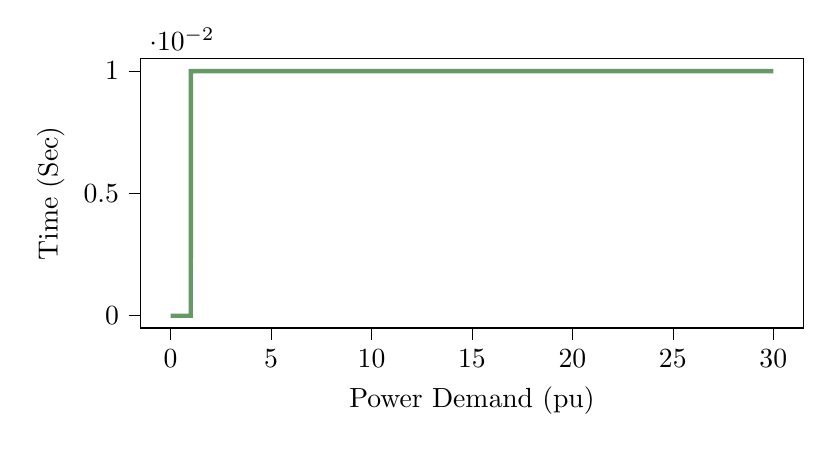
\begin{tikzpicture}

\definecolor{color0}{rgb}{0.12156862745098,0.466666666666667,0.705882352941177}

\begin{axis}[
compat=newest,
tick align=outside,
tick pos=left,
x grid style={white!69.0196078431373!black},
xmin=-1.50000000000009, xmax=31.500000000002,
xtick style={color=black},
y grid style={white!69.0196078431373!black},
ymin=-0.0005, ymax=0.0105,
ytick style={color=black},
scaled y ticks=true,
scaled y ticks=base 10:2,
width=10cm,
height=5cm,
xlabel=Power Demand (pu),
ylabel=Time (Sec)
]
\addplot [ultra thick, green!20!gray]
table {%
0 0
0.01 0
0.02 0
0.03 0
0.04 0
0.05 0
0.06 0
0.07 0
0.08 0
0.09 0
0.1 0
0.11 0
0.12 0
0.13 0
0.14 0
0.15 0
0.16 0
0.17 0
0.18 0
0.19 0
0.2 0
0.21 0
0.22 0
0.23 0
0.24 0
0.25 0
0.26 0
0.27 0
0.28 0
0.29 0
0.3 0
0.31 0
0.32 0
0.33 0
0.34 0
0.35 0
0.36 0
0.37 0
0.38 0
0.39 0
0.4 0
0.41 0
0.42 0
0.43 0
0.44 0
0.45 0
0.46 0
0.47 0
0.48 0
0.49 0
0.5 0
0.51 0
0.52 0
0.53 0
0.54 0
0.55 0
0.56 0
0.57 0
0.58 0
0.59 0
0.6 0
0.61 0
0.62 0
0.63 0
0.64 0
0.65 0
0.66 0
0.67 0
0.68 0
0.69 0
0.7 0
0.71 0
0.72 0
0.73 0
0.74 0
0.75 0
0.76 0
0.77 0
0.78 0
0.79 0
0.8 0
0.81 0
0.820000000000001 0
0.830000000000001 0
0.840000000000001 0
0.850000000000001 0
0.860000000000001 0
0.870000000000001 0
0.880000000000001 0
0.890000000000001 0
0.900000000000001 0
0.910000000000001 0
0.920000000000001 0
0.930000000000001 0
0.940000000000001 0
0.950000000000001 0
0.960000000000001 0
0.970000000000001 0
0.980000000000001 0
0.990000000000001 0
1 0
1.01 0.01
1.02 0.01
1.03 0.01
1.04 0.01
1.05 0.01
1.06 0.01
1.07 0.01
1.08 0.01
1.09 0.01
1.1 0.01
1.11 0.01
1.12 0.01
1.13 0.01
1.14 0.01
1.15 0.01
1.16 0.01
1.17 0.01
1.18 0.01
1.19 0.01
1.2 0.01
1.21 0.01
1.22 0.01
1.23 0.01
1.24 0.01
1.25 0.01
1.26 0.01
1.27 0.01
1.28 0.01
1.29 0.01
1.3 0.01
1.31 0.01
1.32 0.01
1.33 0.01
1.34 0.01
1.35 0.01
1.36 0.01
1.37 0.01
1.38 0.01
1.39 0.01
1.4 0.01
1.41 0.01
1.42 0.01
1.43 0.01
1.44 0.01
1.45 0.01
1.46 0.01
1.47 0.01
1.48 0.01
1.49 0.01
1.5 0.01
1.51 0.01
1.52 0.01
1.53 0.01
1.54 0.01
1.55 0.01
1.56 0.01
1.57 0.01
1.58 0.01
1.59 0.01
1.6 0.01
1.61 0.01
1.62 0.01
1.63 0.01
1.64 0.01
1.65 0.01
1.66 0.01
1.67 0.01
1.68 0.01
1.69 0.01
1.7 0.01
1.71 0.01
1.72 0.01
1.73 0.01
1.74 0.01
1.75 0.01
1.76 0.01
1.77 0.01
1.78 0.01
1.79 0.01
1.8 0.01
1.81 0.01
1.82 0.01
1.83 0.01
1.84 0.01
1.85 0.01
1.86 0.01
1.87 0.01
1.88 0.01
1.89 0.01
1.9 0.01
1.91 0.01
1.92 0.01
1.93 0.01
1.94 0.01
1.95 0.01
1.96 0.01
1.97 0.01
1.98 0.01
1.99 0.01
2 0.01
2.01 0.01
2.02 0.01
2.03 0.01
2.04 0.01
2.05 0.01
2.06 0.01
2.07 0.01
2.08 0.01
2.09 0.01
2.1 0.01
2.11 0.01
2.12 0.01
2.13 0.01
2.14 0.01
2.15 0.01
2.16 0.01
2.17 0.01
2.18 0.01
2.19 0.01
2.2 0.01
2.21 0.01
2.22 0.01
2.23 0.01
2.24 0.01
2.25 0.01
2.26 0.01
2.27 0.01
2.28 0.01
2.29 0.01
2.29999999999999 0.01
2.30999999999999 0.01
2.31999999999999 0.01
2.32999999999999 0.01
2.33999999999999 0.01
2.34999999999999 0.01
2.35999999999999 0.01
2.36999999999999 0.01
2.37999999999999 0.01
2.38999999999999 0.01
2.39999999999999 0.01
2.40999999999999 0.01
2.41999999999999 0.01
2.42999999999999 0.01
2.43999999999999 0.01
2.44999999999999 0.01
2.45999999999999 0.01
2.46999999999999 0.01
2.47999999999999 0.01
2.48999999999999 0.01
2.49999999999999 0.01
2.50999999999999 0.01
2.51999999999999 0.01
2.52999999999999 0.01
2.53999999999999 0.01
2.54999999999999 0.01
2.55999999999999 0.01
2.56999999999999 0.01
2.57999999999999 0.01
2.58999999999999 0.01
2.59999999999999 0.01
2.60999999999999 0.01
2.61999999999999 0.01
2.62999999999999 0.01
2.63999999999999 0.01
2.64999999999999 0.01
2.65999999999999 0.01
2.66999999999999 0.01
2.67999999999999 0.01
2.68999999999999 0.01
2.69999999999999 0.01
2.70999999999999 0.01
2.71999999999999 0.01
2.72999999999999 0.01
2.73999999999999 0.01
2.74999999999999 0.01
2.75999999999999 0.01
2.76999999999998 0.01
2.77999999999998 0.01
2.78999999999998 0.01
2.79999999999998 0.01
2.80999999999998 0.01
2.81999999999998 0.01
2.82999999999998 0.01
2.83999999999998 0.01
2.84999999999998 0.01
2.85999999999998 0.01
2.86999999999998 0.01
2.87999999999998 0.01
2.88999999999998 0.01
2.89999999999998 0.01
2.90999999999998 0.01
2.91999999999998 0.01
2.92999999999998 0.01
2.93999999999998 0.01
2.94999999999998 0.01
2.95999999999998 0.01
2.96999999999998 0.01
2.97999999999998 0.01
2.98999999999998 0.01
2.99999999999998 0.01
3.00999999999998 0.01
3.01999999999998 0.01
3.02999999999998 0.01
3.03999999999998 0.01
3.04999999999998 0.01
3.05999999999998 0.01
3.06999999999998 0.01
3.07999999999998 0.01
3.08999999999998 0.01
3.09999999999998 0.01
3.10999999999998 0.01
3.11999999999998 0.01
3.12999999999998 0.01
3.13999999999998 0.01
3.14999999999998 0.01
3.15999999999998 0.01
3.16999999999998 0.01
3.17999999999998 0.01
3.18999999999998 0.01
3.19999999999998 0.01
3.20999999999998 0.01
3.21999999999998 0.01
3.22999999999998 0.01
3.23999999999997 0.01
3.24999999999997 0.01
3.25999999999997 0.01
3.26999999999997 0.01
3.27999999999997 0.01
3.28999999999997 0.01
3.29999999999997 0.01
3.30999999999997 0.01
3.31999999999997 0.01
3.32999999999997 0.01
3.33999999999997 0.01
3.34999999999997 0.01
3.35999999999997 0.01
3.36999999999997 0.01
3.37999999999997 0.01
3.38999999999997 0.01
3.39999999999997 0.01
3.40999999999997 0.01
3.41999999999997 0.01
3.42999999999997 0.01
3.43999999999997 0.01
3.44999999999997 0.01
3.45999999999997 0.01
3.46999999999997 0.01
3.47999999999997 0.01
3.48999999999997 0.01
3.49999999999997 0.01
3.50999999999997 0.01
3.51999999999997 0.01
3.52999999999997 0.01
3.53999999999997 0.01
3.54999999999997 0.01
3.55999999999997 0.01
3.56999999999997 0.01
3.57999999999997 0.01
3.58999999999997 0.01
3.59999999999997 0.01
3.60999999999997 0.01
3.61999999999997 0.01
3.62999999999997 0.01
3.63999999999997 0.01
3.64999999999997 0.01
3.65999999999997 0.01
3.66999999999997 0.01
3.67999999999997 0.01
3.68999999999997 0.01
3.69999999999997 0.01
3.70999999999996 0.01
3.71999999999996 0.01
3.72999999999996 0.01
3.73999999999996 0.01
3.74999999999996 0.01
3.75999999999996 0.01
3.76999999999996 0.01
3.77999999999996 0.01
3.78999999999996 0.01
3.79999999999996 0.01
3.80999999999996 0.01
3.81999999999996 0.01
3.82999999999996 0.01
3.83999999999996 0.01
3.84999999999996 0.01
3.85999999999996 0.01
3.86999999999996 0.01
3.87999999999996 0.01
3.88999999999996 0.01
3.89999999999996 0.01
3.90999999999996 0.01
3.91999999999996 0.01
3.92999999999996 0.01
3.93999999999996 0.01
3.94999999999996 0.01
3.95999999999996 0.01
3.96999999999996 0.01
3.97999999999996 0.01
3.98999999999996 0.01
3.99999999999996 0.01
4.00999999999996 0.01
4.01999999999996 0.01
4.02999999999996 0.01
4.03999999999996 0.01
4.04999999999996 0.01
4.05999999999996 0.01
4.06999999999996 0.01
4.07999999999996 0.01
4.08999999999996 0.01
4.09999999999996 0.01
4.10999999999996 0.01
4.11999999999996 0.01
4.12999999999996 0.01
4.13999999999996 0.01
4.14999999999996 0.01
4.15999999999996 0.01
4.16999999999996 0.01
4.17999999999996 0.01
4.18999999999996 0.01
4.19999999999995 0.01
4.20999999999995 0.01
4.21999999999995 0.01
4.22999999999995 0.01
4.23999999999995 0.01
4.24999999999995 0.01
4.25999999999995 0.01
4.26999999999995 0.01
4.27999999999995 0.01
4.28999999999995 0.01
4.29999999999995 0.01
4.30999999999995 0.01
4.31999999999995 0.01
4.32999999999995 0.01
4.33999999999995 0.01
4.34999999999995 0.01
4.35999999999995 0.01
4.36999999999995 0.01
4.37999999999995 0.01
4.38999999999995 0.01
4.39999999999995 0.01
4.40999999999995 0.01
4.41999999999995 0.01
4.42999999999995 0.01
4.43999999999995 0.01
4.44999999999995 0.01
4.45999999999995 0.01
4.46999999999995 0.01
4.47999999999995 0.01
4.48999999999995 0.01
4.49999999999995 0.01
4.50999999999995 0.01
4.51999999999995 0.01
4.52999999999995 0.01
4.53999999999995 0.01
4.54999999999995 0.01
4.55999999999995 0.01
4.56999999999995 0.01
4.57999999999995 0.01
4.58999999999995 0.01
4.59999999999995 0.01
4.60999999999995 0.01
4.61999999999995 0.01
4.62999999999995 0.01
4.63999999999995 0.01
4.64999999999995 0.01
4.65999999999995 0.01
4.66999999999994 0.01
4.67999999999994 0.01
4.68999999999994 0.01
4.69999999999994 0.01
4.70999999999994 0.01
4.71999999999994 0.01
4.72999999999994 0.01
4.73999999999994 0.01
4.74999999999994 0.01
4.75999999999994 0.01
4.76999999999994 0.01
4.77999999999994 0.01
4.78999999999994 0.01
4.79999999999994 0.01
4.80999999999994 0.01
4.81999999999994 0.01
4.82999999999994 0.01
4.83999999999994 0.01
4.84999999999994 0.01
4.85999999999994 0.01
4.86999999999994 0.01
4.87999999999994 0.01
4.88999999999994 0.01
4.89999999999994 0.01
4.90999999999994 0.01
4.91999999999994 0.01
4.92999999999994 0.01
4.93999999999994 0.01
4.94999999999994 0.01
4.95999999999994 0.01
4.96999999999994 0.01
4.97999999999994 0.01
4.98999999999994 0.01
4.99999999999994 0.01
5.00999999999994 0.01
5.01999999999994 0.01
5.02999999999994 0.01
5.03999999999994 0.01
5.04999999999994 0.01
5.05999999999994 0.01
5.06999999999994 0.01
5.07999999999994 0.01
5.08999999999994 0.01
5.09999999999994 0.01
5.10999999999994 0.01
5.11999999999994 0.01
5.12999999999994 0.01
5.13999999999993 0.01
5.14999999999993 0.01
5.15999999999993 0.01
5.16999999999993 0.01
5.17999999999993 0.01
5.18999999999993 0.01
5.19999999999993 0.01
5.20999999999993 0.01
5.21999999999993 0.01
5.22999999999993 0.01
5.23999999999993 0.01
5.24999999999993 0.01
5.25999999999993 0.01
5.26999999999993 0.01
5.27999999999993 0.01
5.28999999999993 0.01
5.29999999999993 0.01
5.30999999999993 0.01
5.31999999999993 0.01
5.32999999999993 0.01
5.33999999999993 0.01
5.34999999999993 0.01
5.35999999999993 0.01
5.36999999999993 0.01
5.37999999999993 0.01
5.38999999999993 0.01
5.39999999999993 0.01
5.40999999999993 0.01
5.41999999999993 0.01
5.42999999999993 0.01
5.43999999999993 0.01
5.44999999999993 0.01
5.45999999999993 0.01
5.46999999999993 0.01
5.47999999999993 0.01
5.48999999999993 0.01
5.49999999999993 0.01
5.50999999999993 0.01
5.51999999999993 0.01
5.52999999999993 0.01
5.53999999999993 0.01
5.54999999999993 0.01
5.55999999999993 0.01
5.56999999999993 0.01
5.57999999999993 0.01
5.58999999999993 0.01
5.59999999999993 0.01
5.60999999999992 0.01
5.61999999999992 0.01
5.62999999999992 0.01
5.63999999999992 0.01
5.64999999999992 0.01
5.65999999999992 0.01
5.66999999999992 0.01
5.67999999999992 0.01
5.68999999999992 0.01
5.69999999999992 0.01
5.70999999999992 0.01
5.71999999999992 0.01
5.72999999999992 0.01
5.73999999999992 0.01
5.74999999999992 0.01
5.75999999999992 0.01
5.76999999999992 0.01
5.77999999999992 0.01
5.78999999999992 0.01
5.79999999999992 0.01
5.80999999999992 0.01
5.81999999999992 0.01
5.82999999999992 0.01
5.83999999999992 0.01
5.84999999999992 0.01
5.85999999999992 0.01
5.86999999999992 0.01
5.87999999999992 0.01
5.88999999999992 0.01
5.89999999999992 0.01
5.90999999999992 0.01
5.91999999999992 0.01
5.92999999999992 0.01
5.93999999999992 0.01
5.94999999999992 0.01
5.95999999999992 0.01
5.96999999999992 0.01
5.97999999999992 0.01
5.98999999999992 0.01
5.99999999999992 0.01
6.00999999999992 0.01
6.01999999999992 0.01
6.02999999999992 0.01
6.03999999999992 0.01
6.04999999999992 0.01
6.05999999999992 0.01
6.06999999999992 0.01
6.07999999999991 0.01
6.08999999999991 0.01
6.09999999999991 0.01
6.10999999999991 0.01
6.11999999999991 0.01
6.12999999999991 0.01
6.13999999999991 0.01
6.14999999999991 0.01
6.15999999999991 0.01
6.16999999999991 0.01
6.17999999999991 0.01
6.18999999999991 0.01
6.19999999999991 0.01
6.20999999999991 0.01
6.21999999999991 0.01
6.22999999999991 0.01
6.23999999999991 0.01
6.24999999999991 0.01
6.25999999999991 0.01
6.26999999999991 0.01
6.27999999999991 0.01
6.28999999999991 0.01
6.29999999999991 0.01
6.30999999999991 0.01
6.31999999999991 0.01
6.32999999999991 0.01
6.33999999999991 0.01
6.34999999999991 0.01
6.35999999999991 0.01
6.36999999999991 0.01
6.37999999999991 0.01
6.38999999999991 0.01
6.39999999999991 0.01
6.40999999999991 0.01
6.41999999999991 0.01
6.42999999999991 0.01
6.43999999999991 0.01
6.44999999999991 0.01
6.45999999999991 0.01
6.46999999999991 0.01
6.47999999999991 0.01
6.48999999999991 0.01
6.49999999999991 0.01
6.50999999999991 0.01
6.51999999999991 0.01
6.52999999999991 0.01
6.53999999999991 0.01
6.5499999999999 0.01
6.5599999999999 0.01
6.5699999999999 0.01
6.5799999999999 0.01
6.5899999999999 0.01
6.5999999999999 0.01
6.6099999999999 0.01
6.6199999999999 0.01
6.6299999999999 0.01
6.6399999999999 0.01
6.6499999999999 0.01
6.6599999999999 0.01
6.6699999999999 0.01
6.6799999999999 0.01
6.6899999999999 0.01
6.6999999999999 0.01
6.7099999999999 0.01
6.7199999999999 0.01
6.7299999999999 0.01
6.7399999999999 0.01
6.7499999999999 0.01
6.7599999999999 0.01
6.7699999999999 0.01
6.7799999999999 0.01
6.7899999999999 0.01
6.7999999999999 0.01
6.8099999999999 0.01
6.8199999999999 0.01
6.8299999999999 0.01
6.8399999999999 0.01
6.8499999999999 0.01
6.8599999999999 0.01
6.8699999999999 0.01
6.8799999999999 0.01
6.8899999999999 0.01
6.8999999999999 0.01
6.9099999999999 0.01
6.9199999999999 0.01
6.9299999999999 0.01
6.9399999999999 0.01
6.9499999999999 0.01
6.9599999999999 0.01
6.9699999999999 0.01
6.9799999999999 0.01
6.9899999999999 0.01
6.9999999999999 0.01
7.00999999999989 0.01
7.01999999999989 0.01
7.02999999999989 0.01
7.03999999999989 0.01
7.04999999999989 0.01
7.05999999999989 0.01
7.06999999999989 0.01
7.07999999999989 0.01
7.08999999999989 0.01
7.09999999999989 0.01
7.10999999999989 0.01
7.11999999999989 0.01
7.12999999999989 0.01
7.13999999999989 0.01
7.14999999999989 0.01
7.15999999999989 0.01
7.16999999999989 0.01
7.17999999999989 0.01
7.18999999999989 0.01
7.19999999999989 0.01
7.20999999999989 0.01
7.21999999999989 0.01
7.22999999999989 0.01
7.23999999999989 0.01
7.24999999999989 0.01
7.25999999999989 0.01
7.26999999999989 0.01
7.27999999999989 0.01
7.28999999999989 0.01
7.29999999999989 0.01
7.30999999999989 0.01
7.31999999999989 0.01
7.32999999999989 0.01
7.33999999999989 0.01
7.34999999999989 0.01
7.35999999999989 0.01
7.36999999999989 0.01
7.37999999999989 0.01
7.38999999999989 0.01
7.39999999999989 0.01
7.40999999999989 0.01
7.41999999999989 0.01
7.42999999999989 0.01
7.43999999999989 0.01
7.44999999999989 0.01
7.45999999999989 0.01
7.46999999999989 0.01
7.47999999999988 0.01
7.48999999999988 0.01
7.49999999999988 0.01
7.50999999999988 0.01
7.51999999999988 0.01
7.52999999999988 0.01
7.53999999999988 0.01
7.54999999999988 0.01
7.55999999999988 0.01
7.56999999999988 0.01
7.57999999999988 0.01
7.58999999999988 0.01
7.59999999999988 0.01
7.60999999999988 0.01
7.61999999999988 0.01
7.62999999999988 0.01
7.63999999999988 0.01
7.64999999999988 0.01
7.65999999999988 0.01
7.66999999999988 0.01
7.67999999999988 0.01
7.68999999999988 0.01
7.69999999999988 0.01
7.70999999999988 0.01
7.71999999999988 0.01
7.72999999999988 0.01
7.73999999999988 0.01
7.74999999999988 0.01
7.75999999999988 0.01
7.76999999999988 0.01
7.77999999999988 0.01
7.78999999999988 0.01
7.79999999999988 0.01
7.80999999999988 0.01
7.81999999999988 0.01
7.82999999999988 0.01
7.83999999999988 0.01
7.84999999999988 0.01
7.85999999999988 0.01
7.86999999999988 0.01
7.87999999999988 0.01
7.88999999999988 0.01
7.89999999999988 0.01
7.90999999999988 0.01
7.91999999999988 0.01
7.92999999999988 0.01
7.93999999999988 0.01
7.94999999999987 0.01
7.95999999999987 0.01
7.96999999999987 0.01
7.97999999999987 0.01
7.98999999999987 0.01
7.99999999999987 0.01
8.00999999999987 0.01
8.01999999999987 0.01
8.02999999999987 0.01
8.03999999999987 0.01
8.04999999999987 0.01
8.05999999999987 0.01
8.06999999999987 0.01
8.07999999999987 0.01
8.08999999999987 0.01
8.09999999999987 0.01
8.10999999999987 0.01
8.11999999999987 0.01
8.12999999999987 0.01
8.13999999999987 0.01
8.14999999999987 0.01
8.15999999999987 0.01
8.16999999999987 0.01
8.17999999999987 0.01
8.18999999999987 0.01
8.19999999999987 0.01
8.20999999999987 0.01
8.21999999999987 0.01
8.22999999999987 0.01
8.23999999999987 0.01
8.24999999999987 0.01
8.25999999999987 0.01
8.26999999999987 0.01
8.27999999999987 0.01
8.28999999999987 0.01
8.29999999999987 0.01
8.30999999999987 0.01
8.31999999999987 0.01
8.32999999999987 0.01
8.33999999999987 0.01
8.34999999999987 0.01
8.35999999999987 0.01
8.36999999999987 0.01
8.37999999999987 0.01
8.38999999999987 0.01
8.39999999999987 0.01
8.40999999999987 0.01
8.41999999999986 0.01
8.42999999999986 0.01
8.43999999999986 0.01
8.44999999999986 0.01
8.45999999999986 0.01
8.46999999999986 0.01
8.47999999999986 0.01
8.48999999999986 0.01
8.49999999999986 0.01
8.50999999999986 0.01
8.51999999999986 0.01
8.52999999999986 0.01
8.53999999999986 0.01
8.54999999999986 0.01
8.55999999999986 0.01
8.56999999999986 0.01
8.57999999999986 0.01
8.58999999999986 0.01
8.59999999999986 0.01
8.60999999999986 0.01
8.61999999999986 0.01
8.62999999999986 0.01
8.63999999999986 0.01
8.64999999999986 0.01
8.65999999999986 0.01
8.66999999999986 0.01
8.67999999999986 0.01
8.68999999999986 0.01
8.69999999999986 0.01
8.70999999999986 0.01
8.71999999999986 0.01
8.72999999999986 0.01
8.73999999999986 0.01
8.74999999999986 0.01
8.75999999999986 0.01
8.76999999999986 0.01
8.77999999999986 0.01
8.78999999999986 0.01
8.79999999999986 0.01
8.80999999999986 0.01
8.81999999999986 0.01
8.82999999999986 0.01
8.83999999999986 0.01
8.84999999999986 0.01
8.85999999999986 0.01
8.86999999999986 0.01
8.87999999999986 0.01
8.88999999999985 0.01
8.89999999999985 0.01
8.90999999999985 0.01
8.91999999999985 0.01
8.92999999999985 0.01
8.93999999999985 0.01
8.94999999999985 0.01
8.95999999999985 0.01
8.96999999999985 0.01
8.97999999999985 0.01
8.98999999999985 0.01
8.99999999999985 0.01
9.00999999999985 0.01
9.01999999999985 0.01
9.02999999999985 0.01
9.03999999999985 0.01
9.04999999999985 0.01
9.05999999999985 0.01
9.06999999999985 0.01
9.07999999999985 0.01
9.08999999999985 0.01
9.09999999999985 0.01
9.10999999999985 0.01
9.11999999999985 0.01
9.12999999999985 0.01
9.13999999999985 0.01
9.14999999999985 0.01
9.15999999999985 0.01
9.16999999999985 0.01
9.17999999999985 0.01
9.18999999999985 0.01
9.19999999999985 0.01
9.20999999999985 0.01
9.21999999999985 0.01
9.22999999999985 0.01
9.23999999999985 0.01
9.24999999999985 0.01
9.25999999999985 0.01
9.26999999999985 0.01
9.27999999999985 0.01
9.28999999999985 0.01
9.29999999999985 0.01
9.30999999999985 0.01
9.31999999999985 0.01
9.32999999999985 0.01
9.33999999999985 0.01
9.34999999999985 0.01
9.35999999999984 0.01
9.36999999999984 0.01
9.37999999999984 0.01
9.38999999999984 0.01
9.39999999999984 0.01
9.40999999999984 0.01
9.41999999999984 0.01
9.42999999999984 0.01
9.43999999999984 0.01
9.44999999999984 0.01
9.45999999999984 0.01
9.46999999999984 0.01
9.47999999999984 0.01
9.48999999999984 0.01
9.49999999999984 0.01
9.50999999999984 0.01
9.51999999999984 0.01
9.52999999999984 0.01
9.53999999999984 0.01
9.54999999999984 0.01
9.55999999999984 0.01
9.56999999999984 0.01
9.57999999999984 0.01
9.58999999999984 0.01
9.59999999999984 0.01
9.60999999999984 0.01
9.61999999999984 0.01
9.62999999999984 0.01
9.63999999999984 0.01
9.64999999999984 0.01
9.65999999999984 0.01
9.66999999999984 0.01
9.67999999999984 0.01
9.68999999999984 0.01
9.69999999999984 0.01
9.70999999999984 0.01
9.71999999999984 0.01
9.72999999999984 0.01
9.73999999999984 0.01
9.74999999999984 0.01
9.75999999999984 0.01
9.76999999999984 0.01
9.77999999999984 0.01
9.78999999999984 0.01
9.79999999999984 0.01
9.80999999999984 0.01
9.81999999999984 0.01
9.82999999999983 0.01
9.83999999999983 0.01
9.84999999999983 0.01
9.85999999999983 0.01
9.86999999999983 0.01
9.87999999999983 0.01
9.88999999999983 0.01
9.89999999999983 0.01
9.90999999999983 0.01
9.91999999999983 0.01
9.92999999999983 0.01
9.93999999999983 0.01
9.94999999999983 0.01
9.95999999999983 0.01
9.96999999999983 0.01
9.97999999999983 0.01
9.98999999999983 0.01
9.99999999999983 0.01
10.0099999999998 0.01
10.0199999999998 0.01
10.0299999999998 0.01
10.0399999999998 0.01
10.0499999999998 0.01
10.0599999999998 0.01
10.0699999999998 0.01
10.0799999999998 0.01
10.0899999999998 0.01
10.0999999999998 0.01
10.1099999999998 0.01
10.1199999999998 0.01
10.1299999999998 0.01
10.1399999999998 0.01
10.1499999999998 0.01
10.1599999999998 0.01
10.1699999999998 0.01
10.1799999999998 0.01
10.1899999999998 0.01
10.1999999999998 0.01
10.2099999999998 0.01
10.2199999999998 0.01
10.2299999999998 0.01
10.2399999999998 0.01
10.2499999999998 0.01
10.2599999999998 0.01
10.2699999999998 0.01
10.2799999999998 0.01
10.2899999999998 0.01
10.2999999999998 0.01
10.3099999999998 0.01
10.3199999999998 0.01
10.3299999999998 0.01
10.3399999999998 0.01
10.3499999999998 0.01
10.3599999999998 0.01
10.3699999999998 0.01
10.3799999999998 0.01
10.3899999999998 0.01
10.3999999999998 0.01
10.4099999999998 0.01
10.4199999999998 0.01
10.4299999999998 0.01
10.4399999999998 0.01
10.4499999999998 0.01
10.4599999999998 0.01
10.4699999999998 0.01
10.4799999999998 0.01
10.4899999999998 0.01
10.4999999999998 0.01
10.5099999999998 0.01
10.5199999999998 0.01
10.5299999999998 0.01
10.5399999999998 0.01
10.5499999999998 0.01
10.5599999999998 0.01
10.5699999999998 0.01
10.5799999999998 0.01
10.5899999999998 0.01
10.5999999999998 0.01
10.6099999999998 0.01
10.6199999999998 0.01
10.6299999999998 0.01
10.6399999999998 0.01
10.6499999999998 0.01
10.6599999999998 0.01
10.6699999999998 0.01
10.6799999999998 0.01
10.6899999999998 0.01
10.6999999999998 0.01
10.7099999999998 0.01
10.7199999999998 0.01
10.7299999999998 0.01
10.7399999999998 0.01
10.7499999999998 0.01
10.7599999999998 0.01
10.7699999999998 0.01
10.7799999999998 0.01
10.7899999999998 0.01
10.7999999999998 0.01
10.8099999999998 0.01
10.8199999999998 0.01
10.8299999999998 0.01
10.8399999999998 0.01
10.8499999999998 0.01
10.8599999999998 0.01
10.8699999999998 0.01
10.8799999999998 0.01
10.8899999999998 0.01
10.8999999999998 0.01
10.9099999999998 0.01
10.9199999999998 0.01
10.9299999999998 0.01
10.9399999999998 0.01
10.9499999999998 0.01
10.9599999999998 0.01
10.9699999999998 0.01
10.9799999999998 0.01
10.9899999999998 0.01
10.9999999999998 0.01
11.0099999999998 0.01
11.0199999999998 0.01
11.0299999999998 0.01
11.0399999999998 0.01
11.0499999999998 0.01
11.0599999999998 0.01
11.0699999999998 0.01
11.0799999999998 0.01
11.0899999999998 0.01
11.0999999999998 0.01
11.1099999999998 0.01
11.1199999999998 0.01
11.1299999999998 0.01
11.1399999999998 0.01
11.1499999999998 0.01
11.1599999999998 0.01
11.1699999999998 0.01
11.1799999999998 0.01
11.1899999999998 0.01
11.1999999999998 0.01
11.2099999999998 0.01
11.2199999999998 0.01
11.2299999999998 0.01
11.2399999999998 0.01
11.2499999999998 0.01
11.2599999999998 0.01
11.2699999999998 0.01
11.2799999999998 0.01
11.2899999999998 0.01
11.2999999999998 0.01
11.3099999999998 0.01
11.3199999999998 0.01
11.3299999999998 0.01
11.3399999999998 0.01
11.3499999999998 0.01
11.3599999999998 0.01
11.3699999999998 0.01
11.3799999999998 0.01
11.3899999999998 0.01
11.3999999999998 0.01
11.4099999999998 0.01
11.4199999999998 0.01
11.4299999999998 0.01
11.4399999999998 0.01
11.4499999999998 0.01
11.4599999999998 0.01
11.4699999999998 0.01
11.4799999999998 0.01
11.4899999999998 0.01
11.4999999999998 0.01
11.5099999999998 0.01
11.5199999999998 0.01
11.5299999999998 0.01
11.5399999999998 0.01
11.5499999999998 0.01
11.5599999999998 0.01
11.5699999999998 0.01
11.5799999999998 0.01
11.5899999999998 0.01
11.5999999999998 0.01
11.6099999999998 0.01
11.6199999999998 0.01
11.6299999999998 0.01
11.6399999999998 0.01
11.6499999999998 0.01
11.6599999999998 0.01
11.6699999999998 0.01
11.6799999999998 0.01
11.6899999999998 0.01
11.6999999999998 0.01
11.7099999999998 0.01
11.7199999999998 0.01
11.7299999999998 0.01
11.7399999999998 0.01
11.7499999999998 0.01
11.7599999999998 0.01
11.7699999999998 0.01
11.7799999999998 0.01
11.7899999999998 0.01
11.7999999999998 0.01
11.8099999999998 0.01
11.8199999999998 0.01
11.8299999999998 0.01
11.8399999999998 0.01
11.8499999999998 0.01
11.8599999999998 0.01
11.8699999999998 0.01
11.8799999999998 0.01
11.8899999999998 0.01
11.8999999999998 0.01
11.9099999999998 0.01
11.9199999999998 0.01
11.9299999999998 0.01
11.9399999999998 0.01
11.9499999999998 0.01
11.9599999999998 0.01
11.9699999999998 0.01
11.9799999999998 0.01
11.9899999999998 0.01
11.9999999999998 0.01
12.0099999999998 0.01
12.0199999999998 0.01
12.0299999999998 0.01
12.0399999999998 0.01
12.0499999999998 0.01
12.0599999999998 0.01
12.0699999999998 0.01
12.0799999999998 0.01
12.0899999999998 0.01
12.0999999999998 0.01
12.1099999999998 0.01
12.1199999999998 0.01
12.1299999999998 0.01
12.1399999999998 0.01
12.1499999999998 0.01
12.1599999999998 0.01
12.1699999999998 0.01
12.1799999999998 0.01
12.1899999999998 0.01
12.1999999999998 0.01
12.2099999999998 0.01
12.2199999999998 0.01
12.2299999999998 0.01
12.2399999999998 0.01
12.2499999999998 0.01
12.2599999999998 0.01
12.2699999999998 0.01
12.2799999999998 0.01
12.2899999999998 0.01
12.2999999999998 0.01
12.3099999999998 0.01
12.3199999999998 0.01
12.3299999999998 0.01
12.3399999999998 0.01
12.3499999999998 0.01
12.3599999999998 0.01
12.3699999999998 0.01
12.3799999999998 0.01
12.3899999999998 0.01
12.3999999999998 0.01
12.4099999999998 0.01
12.4199999999998 0.01
12.4299999999998 0.01
12.4399999999998 0.01
12.4499999999998 0.01
12.4599999999998 0.01
12.4699999999998 0.01
12.4799999999998 0.01
12.4899999999998 0.01
12.4999999999998 0.01
12.5099999999998 0.01
12.5199999999998 0.01
12.5299999999998 0.01
12.5399999999998 0.01
12.5499999999998 0.01
12.5599999999998 0.01
12.5699999999998 0.01
12.5799999999998 0.01
12.5899999999998 0.01
12.5999999999998 0.01
12.6099999999998 0.01
12.6199999999998 0.01
12.6299999999998 0.01
12.6399999999998 0.01
12.6499999999998 0.01
12.6599999999998 0.01
12.6699999999998 0.01
12.6799999999998 0.01
12.6899999999998 0.01
12.6999999999998 0.01
12.7099999999998 0.01
12.7199999999998 0.01
12.7299999999998 0.01
12.7399999999998 0.01
12.7499999999998 0.01
12.7599999999998 0.01
12.7699999999998 0.01
12.7799999999998 0.01
12.7899999999998 0.01
12.7999999999998 0.01
12.8099999999998 0.01
12.8199999999998 0.01
12.8299999999998 0.01
12.8399999999998 0.01
12.8499999999998 0.01
12.8599999999998 0.01
12.8699999999998 0.01
12.8799999999998 0.01
12.8899999999998 0.01
12.8999999999998 0.01
12.9099999999998 0.01
12.9199999999998 0.01
12.9299999999998 0.01
12.9399999999998 0.01
12.9499999999998 0.01
12.9599999999998 0.01
12.9699999999998 0.01
12.9799999999998 0.01
12.9899999999998 0.01
12.9999999999998 0.01
13.0099999999998 0.01
13.0199999999998 0.01
13.0299999999998 0.01
13.0399999999998 0.01
13.0499999999998 0.01
13.0599999999998 0.01
13.0699999999998 0.01
13.0799999999998 0.01
13.0899999999998 0.01
13.0999999999998 0.01
13.1099999999998 0.01
13.1199999999998 0.01
13.1299999999998 0.01
13.1399999999998 0.01
13.1499999999998 0.01
13.1599999999998 0.01
13.1699999999998 0.01
13.1799999999998 0.01
13.1899999999998 0.01
13.1999999999998 0.01
13.2099999999998 0.01
13.2199999999998 0.01
13.2299999999998 0.01
13.2399999999998 0.01
13.2499999999998 0.01
13.2599999999998 0.01
13.2699999999998 0.01
13.2799999999998 0.01
13.2899999999998 0.01
13.2999999999998 0.01
13.3099999999998 0.01
13.3199999999998 0.01
13.3299999999998 0.01
13.3399999999998 0.01
13.3499999999998 0.01
13.3599999999998 0.01
13.3699999999998 0.01
13.3799999999998 0.01
13.3899999999998 0.01
13.3999999999998 0.01
13.4099999999998 0.01
13.4199999999998 0.01
13.4299999999998 0.01
13.4399999999998 0.01
13.4499999999998 0.01
13.4599999999998 0.01
13.4699999999998 0.01
13.4799999999998 0.01
13.4899999999998 0.01
13.4999999999998 0.01
13.5099999999998 0.01
13.5199999999998 0.01
13.5299999999998 0.01
13.5399999999998 0.01
13.5499999999998 0.01
13.5599999999998 0.01
13.5699999999998 0.01
13.5799999999998 0.01
13.5899999999998 0.01
13.5999999999998 0.01
13.6099999999998 0.01
13.6199999999998 0.01
13.6299999999998 0.01
13.6399999999998 0.01
13.6499999999998 0.01
13.6599999999998 0.01
13.6699999999998 0.01
13.6799999999998 0.01
13.6899999999998 0.01
13.6999999999998 0.01
13.7099999999998 0.01
13.7199999999998 0.01
13.7299999999998 0.01
13.7399999999998 0.01
13.7499999999998 0.01
13.7599999999998 0.01
13.7699999999998 0.01
13.7799999999998 0.01
13.7899999999998 0.01
13.7999999999998 0.01
13.8099999999998 0.01
13.8199999999997 0.01
13.8299999999997 0.01
13.8399999999997 0.01
13.8499999999997 0.01
13.8599999999997 0.01
13.8699999999997 0.01
13.8799999999997 0.01
13.8899999999997 0.01
13.8999999999997 0.01
13.9099999999997 0.01
13.9199999999997 0.01
13.9299999999997 0.01
13.9399999999997 0.01
13.9499999999997 0.01
13.9599999999997 0.01
13.9699999999997 0.01
13.9799999999997 0.01
13.9899999999997 0.01
13.9999999999997 0.01
14.0099999999997 0.01
14.0199999999997 0.01
14.0299999999997 0.01
14.0399999999997 0.01
14.0499999999997 0.01
14.0599999999997 0.01
14.0699999999997 0.01
14.0799999999997 0.01
14.0899999999997 0.01
14.0999999999997 0.01
14.1099999999997 0.01
14.1199999999997 0.01
14.1299999999997 0.01
14.1399999999997 0.01
14.1499999999997 0.01
14.1599999999997 0.01
14.1699999999997 0.01
14.1799999999997 0.01
14.1899999999997 0.01
14.1999999999997 0.01
14.2099999999997 0.01
14.2199999999997 0.01
14.2299999999997 0.01
14.2399999999997 0.01
14.2499999999997 0.01
14.2599999999997 0.01
14.2699999999997 0.01
14.2799999999997 0.01
14.2899999999997 0.01
14.2999999999997 0.01
14.3099999999997 0.01
14.3199999999997 0.01
14.3299999999997 0.01
14.3399999999997 0.01
14.3499999999997 0.01
14.3599999999997 0.01
14.3699999999997 0.01
14.3799999999997 0.01
14.3899999999997 0.01
14.3999999999997 0.01
14.4099999999997 0.01
14.4199999999997 0.01
14.4299999999997 0.01
14.4399999999997 0.01
14.4499999999997 0.01
14.4599999999997 0.01
14.4699999999997 0.01
14.4799999999997 0.01
14.4899999999997 0.01
14.4999999999997 0.01
14.5099999999997 0.01
14.5199999999997 0.01
14.5299999999997 0.01
14.5399999999997 0.01
14.5499999999997 0.01
14.5599999999997 0.01
14.5699999999997 0.01
14.5799999999997 0.01
14.5899999999997 0.01
14.5999999999997 0.01
14.6099999999997 0.01
14.6199999999997 0.01
14.6299999999997 0.01
14.6399999999997 0.01
14.6499999999997 0.01
14.6599999999997 0.01
14.6699999999997 0.01
14.6799999999997 0.01
14.6899999999997 0.01
14.6999999999997 0.01
14.7099999999997 0.01
14.7199999999997 0.01
14.7299999999997 0.01
14.7399999999997 0.01
14.7499999999997 0.01
14.7599999999997 0.01
14.7699999999997 0.01
14.7799999999997 0.01
14.7899999999997 0.01
14.7999999999997 0.01
14.8099999999997 0.01
14.8199999999997 0.01
14.8299999999997 0.01
14.8399999999997 0.01
14.8499999999997 0.01
14.8599999999997 0.01
14.8699999999997 0.01
14.8799999999997 0.01
14.8899999999997 0.01
14.8999999999997 0.01
14.9099999999997 0.01
14.9199999999997 0.01
14.9299999999997 0.01
14.9399999999997 0.01
14.9499999999997 0.01
14.9599999999997 0.01
14.9699999999997 0.01
14.9799999999997 0.01
14.9899999999997 0.01
14.9999999999997 0.01
15.0099999999997 0.01
15.0199999999997 0.01
15.0299999999997 0.01
15.0399999999997 0.01
15.0499999999997 0.01
15.0599999999997 0.01
15.0699999999997 0.01
15.0799999999997 0.01
15.0899999999997 0.01
15.0999999999997 0.01
15.1099999999997 0.01
15.1199999999997 0.01
15.1299999999997 0.01
15.1399999999997 0.01
15.1499999999997 0.01
15.1599999999997 0.01
15.1699999999997 0.01
15.1799999999997 0.01
15.1899999999997 0.01
15.1999999999997 0.01
15.2099999999997 0.01
15.2199999999997 0.01
15.2299999999997 0.01
15.2399999999997 0.01
15.2499999999997 0.01
15.2599999999997 0.01
15.2699999999997 0.01
15.2799999999997 0.01
15.2899999999997 0.01
15.2999999999997 0.01
15.3099999999997 0.01
15.3199999999997 0.01
15.3299999999997 0.01
15.3399999999997 0.01
15.3499999999997 0.01
15.3599999999997 0.01
15.3699999999997 0.01
15.3799999999997 0.01
15.3899999999997 0.01
15.3999999999997 0.01
15.4099999999997 0.01
15.4199999999997 0.01
15.4299999999997 0.01
15.4399999999997 0.01
15.4499999999997 0.01
15.4599999999997 0.01
15.4699999999997 0.01
15.4799999999997 0.01
15.4899999999997 0.01
15.4999999999997 0.01
15.5099999999997 0.01
15.5199999999997 0.01
15.5299999999997 0.01
15.5399999999997 0.01
15.5499999999997 0.01
15.5599999999997 0.01
15.5699999999997 0.01
15.5799999999997 0.01
15.5899999999997 0.01
15.5999999999997 0.01
15.6099999999997 0.01
15.6199999999997 0.01
15.6299999999997 0.01
15.6399999999997 0.01
15.6499999999997 0.01
15.6599999999997 0.01
15.6699999999997 0.01
15.6799999999997 0.01
15.6899999999997 0.01
15.6999999999997 0.01
15.7099999999997 0.01
15.7199999999997 0.01
15.7299999999997 0.01
15.7399999999997 0.01
15.7499999999997 0.01
15.7599999999997 0.01
15.7699999999997 0.01
15.7799999999997 0.01
15.7899999999997 0.01
15.7999999999997 0.01
15.8099999999997 0.01
15.8199999999997 0.01
15.8299999999997 0.01
15.8399999999997 0.01
15.8499999999997 0.01
15.8599999999997 0.01
15.8699999999997 0.01
15.8799999999997 0.01
15.8899999999997 0.01
15.8999999999997 0.01
15.9099999999997 0.01
15.9199999999997 0.01
15.9299999999997 0.01
15.9399999999997 0.01
15.9499999999997 0.01
15.9599999999997 0.01
15.9699999999997 0.01
15.9799999999997 0.01
15.9899999999997 0.01
15.9999999999997 0.01
16.0099999999997 0.01
16.0199999999997 0.01
16.0299999999997 0.01
16.0399999999997 0.01
16.0499999999997 0.01
16.0599999999997 0.01
16.0699999999997 0.01
16.0799999999997 0.01
16.0899999999997 0.01
16.0999999999997 0.01
16.1099999999997 0.01
16.1199999999997 0.01
16.1299999999997 0.01
16.1399999999997 0.01
16.1499999999997 0.01
16.1599999999997 0.01
16.1699999999997 0.01
16.1799999999997 0.01
16.1899999999997 0.01
16.1999999999997 0.01
16.2099999999997 0.01
16.2199999999997 0.01
16.2299999999997 0.01
16.2399999999997 0.01
16.2499999999997 0.01
16.2599999999997 0.01
16.2699999999997 0.01
16.2799999999997 0.01
16.2899999999997 0.01
16.2999999999997 0.01
16.3099999999998 0.01
16.3199999999998 0.01
16.3299999999998 0.01
16.3399999999998 0.01
16.3499999999998 0.01
16.3599999999998 0.01
16.3699999999998 0.01
16.3799999999998 0.01
16.3899999999998 0.01
16.3999999999998 0.01
16.4099999999998 0.01
16.4199999999998 0.01
16.4299999999998 0.01
16.4399999999998 0.01
16.4499999999998 0.01
16.4599999999998 0.01
16.4699999999998 0.01
16.4799999999998 0.01
16.4899999999998 0.01
16.4999999999998 0.01
16.5099999999998 0.01
16.5199999999998 0.01
16.5299999999998 0.01
16.5399999999998 0.01
16.5499999999998 0.01
16.5599999999998 0.01
16.5699999999998 0.01
16.5799999999998 0.01
16.5899999999998 0.01
16.5999999999998 0.01
16.6099999999998 0.01
16.6199999999998 0.01
16.6299999999998 0.01
16.6399999999998 0.01
16.6499999999998 0.01
16.6599999999998 0.01
16.6699999999998 0.01
16.6799999999998 0.01
16.6899999999998 0.01
16.6999999999998 0.01
16.7099999999998 0.01
16.7199999999998 0.01
16.7299999999998 0.01
16.7399999999998 0.01
16.7499999999998 0.01
16.7599999999998 0.01
16.7699999999998 0.01
16.7799999999998 0.01
16.7899999999998 0.01
16.7999999999998 0.01
16.8099999999998 0.01
16.8199999999998 0.01
16.8299999999998 0.01
16.8399999999998 0.01
16.8499999999998 0.01
16.8599999999998 0.01
16.8699999999998 0.01
16.8799999999998 0.01
16.8899999999998 0.01
16.8999999999998 0.01
16.9099999999998 0.01
16.9199999999998 0.01
16.9299999999998 0.01
16.9399999999998 0.01
16.9499999999999 0.01
16.9599999999999 0.01
16.9699999999999 0.01
16.9799999999999 0.01
16.9899999999999 0.01
16.9999999999999 0.01
17.0099999999999 0.01
17.0199999999999 0.01
17.0299999999999 0.01
17.0399999999999 0.01
17.0499999999999 0.01
17.0599999999999 0.01
17.0699999999999 0.01
17.0799999999999 0.01
17.0899999999999 0.01
17.0999999999999 0.01
17.1099999999999 0.01
17.1199999999999 0.01
17.1299999999999 0.01
17.1399999999999 0.01
17.1499999999999 0.01
17.1599999999999 0.01
17.1699999999999 0.01
17.1799999999999 0.01
17.1899999999999 0.01
17.1999999999999 0.01
17.2099999999999 0.01
17.2199999999999 0.01
17.2299999999999 0.01
17.2399999999999 0.01
17.2499999999999 0.01
17.2599999999999 0.01
17.2699999999999 0.01
17.2799999999999 0.01
17.2899999999999 0.01
17.2999999999999 0.01
17.3099999999999 0.01
17.3199999999999 0.01
17.3299999999999 0.01
17.3399999999999 0.01
17.3499999999999 0.01
17.3599999999999 0.01
17.3699999999999 0.01
17.3799999999999 0.01
17.3899999999999 0.01
17.3999999999999 0.01
17.4099999999999 0.01
17.4199999999999 0.01
17.4299999999999 0.01
17.4399999999999 0.01
17.4499999999999 0.01
17.4599999999999 0.01
17.4699999999999 0.01
17.4799999999999 0.01
17.4899999999999 0.01
17.4999999999999 0.01
17.5099999999999 0.01
17.5199999999999 0.01
17.5299999999999 0.01
17.5399999999999 0.01
17.5499999999999 0.01
17.5599999999999 0.01
17.5699999999999 0.01
17.5799999999999 0.01
17.59 0.01
17.6 0.01
17.61 0.01
17.62 0.01
17.63 0.01
17.64 0.01
17.65 0.01
17.66 0.01
17.67 0.01
17.68 0.01
17.69 0.01
17.7 0.01
17.71 0.01
17.72 0.01
17.73 0.01
17.74 0.01
17.75 0.01
17.76 0.01
17.77 0.01
17.78 0.01
17.79 0.01
17.8 0.01
17.81 0.01
17.82 0.01
17.83 0.01
17.84 0.01
17.85 0.01
17.86 0.01
17.87 0.01
17.88 0.01
17.89 0.01
17.9 0.01
17.91 0.01
17.92 0.01
17.93 0.01
17.94 0.01
17.95 0.01
17.96 0.01
17.97 0.01
17.98 0.01
17.99 0.01
18 0.01
18.01 0.01
18.02 0.01
18.03 0.01
18.04 0.01
18.05 0.01
18.06 0.01
18.07 0.01
18.08 0.01
18.09 0.01
18.1 0.01
18.11 0.01
18.12 0.01
18.13 0.01
18.14 0.01
18.15 0.01
18.16 0.01
18.17 0.01
18.18 0.01
18.19 0.01
18.2 0.01
18.21 0.01
18.22 0.01
18.2300000000001 0.01
18.2400000000001 0.01
18.2500000000001 0.01
18.2600000000001 0.01
18.2700000000001 0.01
18.2800000000001 0.01
18.2900000000001 0.01
18.3000000000001 0.01
18.3100000000001 0.01
18.3200000000001 0.01
18.3300000000001 0.01
18.3400000000001 0.01
18.3500000000001 0.01
18.3600000000001 0.01
18.3700000000001 0.01
18.3800000000001 0.01
18.3900000000001 0.01
18.4000000000001 0.01
18.4100000000001 0.01
18.4200000000001 0.01
18.4300000000001 0.01
18.4400000000001 0.01
18.4500000000001 0.01
18.4600000000001 0.01
18.4700000000001 0.01
18.4800000000001 0.01
18.4900000000001 0.01
18.5000000000001 0.01
18.5100000000001 0.01
18.5200000000001 0.01
18.5300000000001 0.01
18.5400000000001 0.01
18.5500000000001 0.01
18.5600000000001 0.01
18.5700000000001 0.01
18.5800000000001 0.01
18.5900000000001 0.01
18.6000000000001 0.01
18.6100000000001 0.01
18.6200000000001 0.01
18.6300000000001 0.01
18.6400000000001 0.01
18.6500000000001 0.01
18.6600000000001 0.01
18.6700000000001 0.01
18.6800000000001 0.01
18.6900000000001 0.01
18.7000000000001 0.01
18.7100000000001 0.01
18.7200000000001 0.01
18.7300000000001 0.01
18.7400000000001 0.01
18.7500000000001 0.01
18.7600000000001 0.01
18.7700000000001 0.01
18.7800000000001 0.01
18.7900000000001 0.01
18.8000000000001 0.01
18.8100000000001 0.01
18.8200000000001 0.01
18.8300000000001 0.01
18.8400000000001 0.01
18.8500000000001 0.01
18.8600000000001 0.01
18.8700000000002 0.01
18.8800000000002 0.01
18.8900000000002 0.01
18.9000000000002 0.01
18.9100000000002 0.01
18.9200000000002 0.01
18.9300000000002 0.01
18.9400000000002 0.01
18.9500000000002 0.01
18.9600000000002 0.01
18.9700000000002 0.01
18.9800000000002 0.01
18.9900000000002 0.01
19.0000000000002 0.01
19.0100000000002 0.01
19.0200000000002 0.01
19.0300000000002 0.01
19.0400000000002 0.01
19.0500000000002 0.01
19.0600000000002 0.01
19.0700000000002 0.01
19.0800000000002 0.01
19.0900000000002 0.01
19.1000000000002 0.01
19.1100000000002 0.01
19.1200000000002 0.01
19.1300000000002 0.01
19.1400000000002 0.01
19.1500000000002 0.01
19.1600000000002 0.01
19.1700000000002 0.01
19.1800000000002 0.01
19.1900000000002 0.01
19.2000000000002 0.01
19.2100000000002 0.01
19.2200000000002 0.01
19.2300000000002 0.01
19.2400000000002 0.01
19.2500000000002 0.01
19.2600000000002 0.01
19.2700000000002 0.01
19.2800000000002 0.01
19.2900000000002 0.01
19.3000000000002 0.01
19.3100000000002 0.01
19.3200000000002 0.01
19.3300000000002 0.01
19.3400000000002 0.01
19.3500000000002 0.01
19.3600000000002 0.01
19.3700000000002 0.01
19.3800000000002 0.01
19.3900000000002 0.01
19.4000000000002 0.01
19.4100000000002 0.01
19.4200000000002 0.01
19.4300000000002 0.01
19.4400000000002 0.01
19.4500000000002 0.01
19.4600000000002 0.01
19.4700000000002 0.01
19.4800000000002 0.01
19.4900000000002 0.01
19.5000000000002 0.01
19.5100000000003 0.01
19.5200000000003 0.01
19.5300000000003 0.01
19.5400000000003 0.01
19.5500000000003 0.01
19.5600000000003 0.01
19.5700000000003 0.01
19.5800000000003 0.01
19.5900000000003 0.01
19.6000000000003 0.01
19.6100000000003 0.01
19.6200000000003 0.01
19.6300000000003 0.01
19.6400000000003 0.01
19.6500000000003 0.01
19.6600000000003 0.01
19.6700000000003 0.01
19.6800000000003 0.01
19.6900000000003 0.01
19.7000000000003 0.01
19.7100000000003 0.01
19.7200000000003 0.01
19.7300000000003 0.01
19.7400000000003 0.01
19.7500000000003 0.01
19.7600000000003 0.01
19.7700000000003 0.01
19.7800000000003 0.01
19.7900000000003 0.01
19.8000000000003 0.01
19.8100000000003 0.01
19.8200000000003 0.01
19.8300000000003 0.01
19.8400000000003 0.01
19.8500000000003 0.01
19.8600000000003 0.01
19.8700000000003 0.01
19.8800000000003 0.01
19.8900000000003 0.01
19.9000000000003 0.01
19.9100000000003 0.01
19.9200000000003 0.01
19.9300000000003 0.01
19.9400000000003 0.01
19.9500000000003 0.01
19.9600000000003 0.01
19.9700000000003 0.01
19.9800000000003 0.01
19.9900000000003 0.01
20.0000000000003 0.01
20.0100000000003 0.01
20.0200000000003 0.01
20.0300000000003 0.01
20.0400000000003 0.01
20.0500000000003 0.01
20.0600000000003 0.01
20.0700000000003 0.01
20.0800000000003 0.01
20.0900000000003 0.01
20.1000000000003 0.01
20.1100000000003 0.01
20.1200000000003 0.01
20.1300000000003 0.01
20.1400000000003 0.01
20.1500000000004 0.01
20.1600000000004 0.01
20.1700000000004 0.01
20.1800000000004 0.01
20.1900000000004 0.01
20.2000000000004 0.01
20.2100000000004 0.01
20.2200000000004 0.01
20.2300000000004 0.01
20.2400000000004 0.01
20.2500000000004 0.01
20.2600000000004 0.01
20.2700000000004 0.01
20.2800000000004 0.01
20.2900000000004 0.01
20.3000000000004 0.01
20.3100000000004 0.01
20.3200000000004 0.01
20.3300000000004 0.01
20.3400000000004 0.01
20.3500000000004 0.01
20.3600000000004 0.01
20.3700000000004 0.01
20.3800000000004 0.01
20.3900000000004 0.01
20.4000000000004 0.01
20.4100000000004 0.01
20.4200000000004 0.01
20.4300000000004 0.01
20.4400000000004 0.01
20.4500000000004 0.01
20.4600000000004 0.01
20.4700000000004 0.01
20.4800000000004 0.01
20.4900000000004 0.01
20.5000000000004 0.01
20.5100000000004 0.01
20.5200000000004 0.01
20.5300000000004 0.01
20.5400000000004 0.01
20.5500000000004 0.01
20.5600000000004 0.01
20.5700000000004 0.01
20.5800000000004 0.01
20.5900000000004 0.01
20.6000000000004 0.01
20.6100000000004 0.01
20.6200000000004 0.01
20.6300000000004 0.01
20.6400000000004 0.01
20.6500000000004 0.01
20.6600000000004 0.01
20.6700000000004 0.01
20.6800000000004 0.01
20.6900000000004 0.01
20.7000000000004 0.01
20.7100000000004 0.01
20.7200000000004 0.01
20.7300000000004 0.01
20.7400000000004 0.01
20.7500000000004 0.01
20.7600000000004 0.01
20.7700000000004 0.01
20.7800000000004 0.01
20.7900000000005 0.01
20.8000000000005 0.01
20.8100000000005 0.01
20.8200000000005 0.01
20.8300000000005 0.01
20.8400000000005 0.01
20.8500000000005 0.01
20.8600000000005 0.01
20.8700000000005 0.01
20.8800000000005 0.01
20.8900000000005 0.01
20.9000000000005 0.01
20.9100000000005 0.01
20.9200000000005 0.01
20.9300000000005 0.01
20.9400000000005 0.01
20.9500000000005 0.01
20.9600000000005 0.01
20.9700000000005 0.01
20.9800000000005 0.01
20.9900000000005 0.01
21.0000000000005 0.01
21.0100000000005 0.01
21.0200000000005 0.01
21.0300000000005 0.01
21.0400000000005 0.01
21.0500000000005 0.01
21.0600000000005 0.01
21.0700000000005 0.01
21.0800000000005 0.01
21.0900000000005 0.01
21.1000000000005 0.01
21.1100000000005 0.01
21.1200000000005 0.01
21.1300000000005 0.01
21.1400000000005 0.01
21.1500000000005 0.01
21.1600000000005 0.01
21.1700000000005 0.01
21.1800000000005 0.01
21.1900000000005 0.01
21.2000000000005 0.01
21.2100000000005 0.01
21.2200000000005 0.01
21.2300000000005 0.01
21.2400000000005 0.01
21.2500000000005 0.01
21.2600000000005 0.01
21.2700000000005 0.01
21.2800000000005 0.01
21.2900000000005 0.01
21.3000000000005 0.01
21.3100000000005 0.01
21.3200000000005 0.01
21.3300000000005 0.01
21.3400000000005 0.01
21.3500000000005 0.01
21.3600000000005 0.01
21.3700000000005 0.01
21.3800000000005 0.01
21.3900000000005 0.01
21.4000000000005 0.01
21.4100000000005 0.01
21.4200000000005 0.01
21.4300000000006 0.01
21.4400000000006 0.01
21.4500000000006 0.01
21.4600000000006 0.01
21.4700000000006 0.01
21.4800000000006 0.01
21.4900000000006 0.01
21.5000000000006 0.01
21.5100000000006 0.01
21.5200000000006 0.01
21.5300000000006 0.01
21.5400000000006 0.01
21.5500000000006 0.01
21.5600000000006 0.01
21.5700000000006 0.01
21.5800000000006 0.01
21.5900000000006 0.01
21.6000000000006 0.01
21.6100000000006 0.01
21.6200000000006 0.01
21.6300000000006 0.01
21.6400000000006 0.01
21.6500000000006 0.01
21.6600000000006 0.01
21.6700000000006 0.01
21.6800000000006 0.01
21.6900000000006 0.01
21.7000000000006 0.01
21.7100000000006 0.01
21.7200000000006 0.01
21.7300000000006 0.01
21.7400000000006 0.01
21.7500000000006 0.01
21.7600000000006 0.01
21.7700000000006 0.01
21.7800000000006 0.01
21.7900000000006 0.01
21.8000000000006 0.01
21.8100000000006 0.01
21.8200000000006 0.01
21.8300000000006 0.01
21.8400000000006 0.01
21.8500000000006 0.01
21.8600000000006 0.01
21.8700000000006 0.01
21.8800000000006 0.01
21.8900000000006 0.01
21.9000000000006 0.01
21.9100000000006 0.01
21.9200000000006 0.01
21.9300000000006 0.01
21.9400000000006 0.01
21.9500000000006 0.01
21.9600000000006 0.01
21.9700000000006 0.01
21.9800000000006 0.01
21.9900000000006 0.01
22.0000000000006 0.01
22.0100000000006 0.01
22.0200000000006 0.01
22.0300000000006 0.01
22.0400000000006 0.01
22.0500000000006 0.01
22.0600000000006 0.01
22.0700000000007 0.01
22.0800000000007 0.01
22.0900000000007 0.01
22.1000000000007 0.01
22.1100000000007 0.01
22.1200000000007 0.01
22.1300000000007 0.01
22.1400000000007 0.01
22.1500000000007 0.01
22.1600000000007 0.01
22.1700000000007 0.01
22.1800000000007 0.01
22.1900000000007 0.01
22.2000000000007 0.01
22.2100000000007 0.01
22.2200000000007 0.01
22.2300000000007 0.01
22.2400000000007 0.01
22.2500000000007 0.01
22.2600000000007 0.01
22.2700000000007 0.01
22.2800000000007 0.01
22.2900000000007 0.01
22.3000000000007 0.01
22.3100000000007 0.01
22.3200000000007 0.01
22.3300000000007 0.01
22.3400000000007 0.01
22.3500000000007 0.01
22.3600000000007 0.01
22.3700000000007 0.01
22.3800000000007 0.01
22.3900000000007 0.01
22.4000000000007 0.01
22.4100000000007 0.01
22.4200000000007 0.01
22.4300000000007 0.01
22.4400000000007 0.01
22.4500000000007 0.01
22.4600000000007 0.01
22.4700000000007 0.01
22.4800000000007 0.01
22.4900000000007 0.01
22.5000000000007 0.01
22.5100000000007 0.01
22.5200000000007 0.01
22.5300000000007 0.01
22.5400000000007 0.01
22.5500000000007 0.01
22.5600000000007 0.01
22.5700000000007 0.01
22.5800000000007 0.01
22.5900000000007 0.01
22.6000000000007 0.01
22.6100000000007 0.01
22.6200000000007 0.01
22.6300000000007 0.01
22.6400000000007 0.01
22.6500000000007 0.01
22.6600000000007 0.01
22.6700000000007 0.01
22.6800000000007 0.01
22.6900000000007 0.01
22.7000000000007 0.01
22.7100000000008 0.01
22.7200000000008 0.01
22.7300000000008 0.01
22.7400000000008 0.01
22.7500000000008 0.01
22.7600000000008 0.01
22.7700000000008 0.01
22.7800000000008 0.01
22.7900000000008 0.01
22.8000000000008 0.01
22.8100000000008 0.01
22.8200000000008 0.01
22.8300000000008 0.01
22.8400000000008 0.01
22.8500000000008 0.01
22.8600000000008 0.01
22.8700000000008 0.01
22.8800000000008 0.01
22.8900000000008 0.01
22.9000000000008 0.01
22.9100000000008 0.01
22.9200000000008 0.01
22.9300000000008 0.01
22.9400000000008 0.01
22.9500000000008 0.01
22.9600000000008 0.01
22.9700000000008 0.01
22.9800000000008 0.01
22.9900000000008 0.01
23.0000000000008 0.01
23.0100000000008 0.01
23.0200000000008 0.01
23.0300000000008 0.01
23.0400000000008 0.01
23.0500000000008 0.01
23.0600000000008 0.01
23.0700000000008 0.01
23.0800000000008 0.01
23.0900000000008 0.01
23.1000000000008 0.01
23.1100000000008 0.01
23.1200000000008 0.01
23.1300000000008 0.01
23.1400000000008 0.01
23.1500000000008 0.01
23.1600000000008 0.01
23.1700000000008 0.01
23.1800000000008 0.01
23.1900000000008 0.01
23.2000000000008 0.01
23.2100000000008 0.01
23.2200000000008 0.01
23.2300000000008 0.01
23.2400000000008 0.01
23.2500000000008 0.01
23.2600000000008 0.01
23.2700000000008 0.01
23.2800000000008 0.01
23.2900000000008 0.01
23.3000000000008 0.01
23.3100000000008 0.01
23.3200000000008 0.01
23.3300000000008 0.01
23.3400000000008 0.01
23.3500000000009 0.01
23.3600000000009 0.01
23.3700000000009 0.01
23.3800000000009 0.01
23.3900000000009 0.01
23.4000000000009 0.01
23.4100000000009 0.01
23.4200000000009 0.01
23.4300000000009 0.01
23.4400000000009 0.01
23.4500000000009 0.01
23.4600000000009 0.01
23.4700000000009 0.01
23.4800000000009 0.01
23.4900000000009 0.01
23.5000000000009 0.01
23.5100000000009 0.01
23.5200000000009 0.01
23.5300000000009 0.01
23.5400000000009 0.01
23.5500000000009 0.01
23.5600000000009 0.01
23.5700000000009 0.01
23.5800000000009 0.01
23.5900000000009 0.01
23.6000000000009 0.01
23.6100000000009 0.01
23.6200000000009 0.01
23.6300000000009 0.01
23.6400000000009 0.01
23.6500000000009 0.01
23.6600000000009 0.01
23.6700000000009 0.01
23.6800000000009 0.01
23.6900000000009 0.01
23.7000000000009 0.01
23.7100000000009 0.01
23.7200000000009 0.01
23.7300000000009 0.01
23.7400000000009 0.01
23.7500000000009 0.01
23.7600000000009 0.01
23.7700000000009 0.01
23.7800000000009 0.01
23.7900000000009 0.01
23.8000000000009 0.01
23.8100000000009 0.01
23.8200000000009 0.01
23.8300000000009 0.01
23.8400000000009 0.01
23.8500000000009 0.01
23.8600000000009 0.01
23.8700000000009 0.01
23.8800000000009 0.01
23.8900000000009 0.01
23.9000000000009 0.01
23.9100000000009 0.01
23.9200000000009 0.01
23.9300000000009 0.01
23.9400000000009 0.01
23.9500000000009 0.01
23.9600000000009 0.01
23.9700000000009 0.01
23.9800000000009 0.01
23.990000000001 0.01
24.000000000001 0.01
24.010000000001 0.01
24.020000000001 0.01
24.030000000001 0.01
24.040000000001 0.01
24.050000000001 0.01
24.060000000001 0.01
24.070000000001 0.01
24.080000000001 0.01
24.090000000001 0.01
24.100000000001 0.01
24.110000000001 0.01
24.120000000001 0.01
24.130000000001 0.01
24.140000000001 0.01
24.150000000001 0.01
24.160000000001 0.01
24.170000000001 0.01
24.180000000001 0.01
24.190000000001 0.01
24.200000000001 0.01
24.210000000001 0.01
24.220000000001 0.01
24.230000000001 0.01
24.240000000001 0.01
24.250000000001 0.01
24.260000000001 0.01
24.270000000001 0.01
24.280000000001 0.01
24.290000000001 0.01
24.300000000001 0.01
24.310000000001 0.01
24.320000000001 0.01
24.330000000001 0.01
24.340000000001 0.01
24.350000000001 0.01
24.360000000001 0.01
24.370000000001 0.01
24.380000000001 0.01
24.390000000001 0.01
24.400000000001 0.01
24.410000000001 0.01
24.420000000001 0.01
24.430000000001 0.01
24.440000000001 0.01
24.450000000001 0.01
24.460000000001 0.01
24.470000000001 0.01
24.480000000001 0.01
24.490000000001 0.01
24.500000000001 0.01
24.510000000001 0.01
24.520000000001 0.01
24.530000000001 0.01
24.540000000001 0.01
24.550000000001 0.01
24.560000000001 0.01
24.570000000001 0.01
24.580000000001 0.01
24.590000000001 0.01
24.600000000001 0.01
24.610000000001 0.01
24.620000000001 0.01
24.6300000000011 0.01
24.6400000000011 0.01
24.6500000000011 0.01
24.6600000000011 0.01
24.6700000000011 0.01
24.6800000000011 0.01
24.6900000000011 0.01
24.7000000000011 0.01
24.7100000000011 0.01
24.7200000000011 0.01
24.7300000000011 0.01
24.7400000000011 0.01
24.7500000000011 0.01
24.7600000000011 0.01
24.7700000000011 0.01
24.7800000000011 0.01
24.7900000000011 0.01
24.8000000000011 0.01
24.8100000000011 0.01
24.8200000000011 0.01
24.8300000000011 0.01
24.8400000000011 0.01
24.8500000000011 0.01
24.8600000000011 0.01
24.8700000000011 0.01
24.8800000000011 0.01
24.8900000000011 0.01
24.9000000000011 0.01
24.9100000000011 0.01
24.9200000000011 0.01
24.9300000000011 0.01
24.9400000000011 0.01
24.9500000000011 0.01
24.9600000000011 0.01
24.9700000000011 0.01
24.9800000000011 0.01
24.9900000000011 0.01
25.0000000000011 0.01
25.0100000000011 0.01
25.0200000000011 0.01
25.0300000000011 0.01
25.0400000000011 0.01
25.0500000000011 0.01
25.0600000000011 0.01
25.0700000000011 0.01
25.0800000000011 0.01
25.0900000000011 0.01
25.1000000000011 0.01
25.1100000000011 0.01
25.1200000000011 0.01
25.1300000000011 0.01
25.1400000000011 0.01
25.1500000000011 0.01
25.1600000000011 0.01
25.1700000000011 0.01
25.1800000000011 0.01
25.1900000000011 0.01
25.2000000000011 0.01
25.2100000000011 0.01
25.2200000000011 0.01
25.2300000000011 0.01
25.2400000000011 0.01
25.2500000000011 0.01
25.2600000000011 0.01
25.2700000000012 0.01
25.2800000000012 0.01
25.2900000000012 0.01
25.3000000000012 0.01
25.3100000000012 0.01
25.3200000000012 0.01
25.3300000000012 0.01
25.3400000000012 0.01
25.3500000000012 0.01
25.3600000000012 0.01
25.3700000000012 0.01
25.3800000000012 0.01
25.3900000000012 0.01
25.4000000000012 0.01
25.4100000000012 0.01
25.4200000000012 0.01
25.4300000000012 0.01
25.4400000000012 0.01
25.4500000000012 0.01
25.4600000000012 0.01
25.4700000000012 0.01
25.4800000000012 0.01
25.4900000000012 0.01
25.5000000000012 0.01
25.5100000000012 0.01
25.5200000000012 0.01
25.5300000000012 0.01
25.5400000000012 0.01
25.5500000000012 0.01
25.5600000000012 0.01
25.5700000000012 0.01
25.5800000000012 0.01
25.5900000000012 0.01
25.6000000000012 0.01
25.6100000000012 0.01
25.6200000000012 0.01
25.6300000000012 0.01
25.6400000000012 0.01
25.6500000000012 0.01
25.6600000000012 0.01
25.6700000000012 0.01
25.6800000000012 0.01
25.6900000000012 0.01
25.7000000000012 0.01
25.7100000000012 0.01
25.7200000000012 0.01
25.7300000000012 0.01
25.7400000000012 0.01
25.7500000000012 0.01
25.7600000000012 0.01
25.7700000000012 0.01
25.7800000000012 0.01
25.7900000000012 0.01
25.8000000000012 0.01
25.8100000000012 0.01
25.8200000000012 0.01
25.8300000000012 0.01
25.8400000000012 0.01
25.8500000000012 0.01
25.8600000000012 0.01
25.8700000000012 0.01
25.8800000000012 0.01
25.8900000000012 0.01
25.9000000000012 0.01
25.9100000000013 0.01
25.9200000000013 0.01
25.9300000000013 0.01
25.9400000000013 0.01
25.9500000000013 0.01
25.9600000000013 0.01
25.9700000000013 0.01
25.9800000000013 0.01
25.9900000000013 0.01
26.0000000000013 0.01
26.0100000000013 0.01
26.0200000000013 0.01
26.0300000000013 0.01
26.0400000000013 0.01
26.0500000000013 0.01
26.0600000000013 0.01
26.0700000000013 0.01
26.0800000000013 0.01
26.0900000000013 0.01
26.1000000000013 0.01
26.1100000000013 0.01
26.1200000000013 0.01
26.1300000000013 0.01
26.1400000000013 0.01
26.1500000000013 0.01
26.1600000000013 0.01
26.1700000000013 0.01
26.1800000000013 0.01
26.1900000000013 0.01
26.2000000000013 0.01
26.2100000000013 0.01
26.2200000000013 0.01
26.2300000000013 0.01
26.2400000000013 0.01
26.2500000000013 0.01
26.2600000000013 0.01
26.2700000000013 0.01
26.2800000000013 0.01
26.2900000000013 0.01
26.3000000000013 0.01
26.3100000000013 0.01
26.3200000000013 0.01
26.3300000000013 0.01
26.3400000000013 0.01
26.3500000000013 0.01
26.3600000000013 0.01
26.3700000000013 0.01
26.3800000000013 0.01
26.3900000000013 0.01
26.4000000000013 0.01
26.4100000000013 0.01
26.4200000000013 0.01
26.4300000000013 0.01
26.4400000000013 0.01
26.4500000000013 0.01
26.4600000000013 0.01
26.4700000000013 0.01
26.4800000000013 0.01
26.4900000000013 0.01
26.5000000000013 0.01
26.5100000000013 0.01
26.5200000000013 0.01
26.5300000000013 0.01
26.5400000000013 0.01
26.5500000000014 0.01
26.5600000000014 0.01
26.5700000000014 0.01
26.5800000000014 0.01
26.5900000000014 0.01
26.6000000000014 0.01
26.6100000000014 0.01
26.6200000000014 0.01
26.6300000000014 0.01
26.6400000000014 0.01
26.6500000000014 0.01
26.6600000000014 0.01
26.6700000000014 0.01
26.6800000000014 0.01
26.6900000000014 0.01
26.7000000000014 0.01
26.7100000000014 0.01
26.7200000000014 0.01
26.7300000000014 0.01
26.7400000000014 0.01
26.7500000000014 0.01
26.7600000000014 0.01
26.7700000000014 0.01
26.7800000000014 0.01
26.7900000000014 0.01
26.8000000000014 0.01
26.8100000000014 0.01
26.8200000000014 0.01
26.8300000000014 0.01
26.8400000000014 0.01
26.8500000000014 0.01
26.8600000000014 0.01
26.8700000000014 0.01
26.8800000000014 0.01
26.8900000000014 0.01
26.9000000000014 0.01
26.9100000000014 0.01
26.9200000000014 0.01
26.9300000000014 0.01
26.9400000000014 0.01
26.9500000000014 0.01
26.9600000000014 0.01
26.9700000000014 0.01
26.9800000000014 0.01
26.9900000000014 0.01
27.0000000000014 0.01
27.0100000000014 0.01
27.0200000000014 0.01
27.0300000000014 0.01
27.0400000000014 0.01
27.0500000000014 0.01
27.0600000000014 0.01
27.0700000000014 0.01
27.0800000000014 0.01
27.0900000000014 0.01
27.1000000000014 0.01
27.1100000000014 0.01
27.1200000000014 0.01
27.1300000000014 0.01
27.1400000000014 0.01
27.1500000000014 0.01
27.1600000000014 0.01
27.1700000000014 0.01
27.1800000000014 0.01
27.1900000000015 0.01
27.2000000000015 0.01
27.2100000000015 0.01
27.2200000000015 0.01
27.2300000000015 0.01
27.2400000000015 0.01
27.2500000000015 0.01
27.2600000000015 0.01
27.2700000000015 0.01
27.2800000000015 0.01
27.2900000000015 0.01
27.3000000000015 0.01
27.3100000000015 0.01
27.3200000000015 0.01
27.3300000000015 0.01
27.3400000000015 0.01
27.3500000000015 0.01
27.3600000000015 0.01
27.3700000000015 0.01
27.3800000000015 0.01
27.3900000000015 0.01
27.4000000000015 0.01
27.4100000000015 0.01
27.4200000000015 0.01
27.4300000000015 0.01
27.4400000000015 0.01
27.4500000000015 0.01
27.4600000000015 0.01
27.4700000000015 0.01
27.4800000000015 0.01
27.4900000000015 0.01
27.5000000000015 0.01
27.5100000000015 0.01
27.5200000000015 0.01
27.5300000000015 0.01
27.5400000000015 0.01
27.5500000000015 0.01
27.5600000000015 0.01
27.5700000000015 0.01
27.5800000000015 0.01
27.5900000000015 0.01
27.6000000000015 0.01
27.6100000000015 0.01
27.6200000000015 0.01
27.6300000000015 0.01
27.6400000000015 0.01
27.6500000000015 0.01
27.6600000000015 0.01
27.6700000000015 0.01
27.6800000000015 0.01
27.6900000000015 0.01
27.7000000000015 0.01
27.7100000000015 0.01
27.7200000000015 0.01
27.7300000000015 0.01
27.7400000000015 0.01
27.7500000000015 0.01
27.7600000000015 0.01
27.7700000000015 0.01
27.7800000000015 0.01
27.7900000000015 0.01
27.8000000000015 0.01
27.8100000000015 0.01
27.8200000000015 0.01
27.8300000000016 0.01
27.8400000000016 0.01
27.8500000000016 0.01
27.8600000000016 0.01
27.8700000000016 0.01
27.8800000000016 0.01
27.8900000000016 0.01
27.9000000000016 0.01
27.9100000000016 0.01
27.9200000000016 0.01
27.9300000000016 0.01
27.9400000000016 0.01
27.9500000000016 0.01
27.9600000000016 0.01
27.9700000000016 0.01
27.9800000000016 0.01
27.9900000000016 0.01
28.0000000000016 0.01
28.0100000000016 0.01
28.0200000000016 0.01
28.0300000000016 0.01
28.0400000000016 0.01
28.0500000000016 0.01
28.0600000000016 0.01
28.0700000000016 0.01
28.0800000000016 0.01
28.0900000000016 0.01
28.1000000000016 0.01
28.1100000000016 0.01
28.1200000000016 0.01
28.1300000000016 0.01
28.1400000000016 0.01
28.1500000000016 0.01
28.1600000000016 0.01
28.1700000000016 0.01
28.1800000000016 0.01
28.1900000000016 0.01
28.2000000000016 0.01
28.2100000000016 0.01
28.2200000000016 0.01
28.2300000000016 0.01
28.2400000000016 0.01
28.2500000000016 0.01
28.2600000000016 0.01
28.2700000000016 0.01
28.2800000000016 0.01
28.2900000000016 0.01
28.3000000000016 0.01
28.3100000000016 0.01
28.3200000000016 0.01
28.3300000000016 0.01
28.3400000000016 0.01
28.3500000000016 0.01
28.3600000000016 0.01
28.3700000000016 0.01
28.3800000000016 0.01
28.3900000000016 0.01
28.4000000000016 0.01
28.4100000000016 0.01
28.4200000000016 0.01
28.4300000000016 0.01
28.4400000000016 0.01
28.4500000000016 0.01
28.4600000000016 0.01
28.4700000000017 0.01
28.4800000000017 0.01
28.4900000000017 0.01
28.5000000000017 0.01
28.5100000000017 0.01
28.5200000000017 0.01
28.5300000000017 0.01
28.5400000000017 0.01
28.5500000000017 0.01
28.5600000000017 0.01
28.5700000000017 0.01
28.5800000000017 0.01
28.5900000000017 0.01
28.6000000000017 0.01
28.6100000000017 0.01
28.6200000000017 0.01
28.6300000000017 0.01
28.6400000000017 0.01
28.6500000000017 0.01
28.6600000000017 0.01
28.6700000000017 0.01
28.6800000000017 0.01
28.6900000000017 0.01
28.7000000000017 0.01
28.7100000000017 0.01
28.7200000000017 0.01
28.7300000000017 0.01
28.7400000000017 0.01
28.7500000000017 0.01
28.7600000000017 0.01
28.7700000000017 0.01
28.7800000000017 0.01
28.7900000000017 0.01
28.8000000000017 0.01
28.8100000000017 0.01
28.8200000000017 0.01
28.8300000000017 0.01
28.8400000000017 0.01
28.8500000000017 0.01
28.8600000000017 0.01
28.8700000000017 0.01
28.8800000000017 0.01
28.8900000000017 0.01
28.9000000000017 0.01
28.9100000000017 0.01
28.9200000000017 0.01
28.9300000000017 0.01
28.9400000000017 0.01
28.9500000000017 0.01
28.9600000000017 0.01
28.9700000000017 0.01
28.9800000000017 0.01
28.9900000000017 0.01
29.0000000000017 0.01
29.0100000000017 0.01
29.0200000000017 0.01
29.0300000000017 0.01
29.0400000000017 0.01
29.0500000000017 0.01
29.0600000000017 0.01
29.0700000000017 0.01
29.0800000000017 0.01
29.0900000000017 0.01
29.1000000000017 0.01
29.1100000000018 0.01
29.1200000000018 0.01
29.1300000000018 0.01
29.1400000000018 0.01
29.1500000000018 0.01
29.1600000000018 0.01
29.1700000000018 0.01
29.1800000000018 0.01
29.1900000000018 0.01
29.2000000000018 0.01
29.2100000000018 0.01
29.2200000000018 0.01
29.2300000000018 0.01
29.2400000000018 0.01
29.2500000000018 0.01
29.2600000000018 0.01
29.2700000000018 0.01
29.2800000000018 0.01
29.2900000000018 0.01
29.3000000000018 0.01
29.3100000000018 0.01
29.3200000000018 0.01
29.3300000000018 0.01
29.3400000000018 0.01
29.3500000000018 0.01
29.3600000000018 0.01
29.3700000000018 0.01
29.3800000000018 0.01
29.3900000000018 0.01
29.4000000000018 0.01
29.4100000000018 0.01
29.4200000000018 0.01
29.4300000000018 0.01
29.4400000000018 0.01
29.4500000000018 0.01
29.4600000000018 0.01
29.4700000000018 0.01
29.4800000000018 0.01
29.4900000000018 0.01
29.5000000000018 0.01
29.5100000000018 0.01
29.5200000000018 0.01
29.5300000000018 0.01
29.5400000000018 0.01
29.5500000000018 0.01
29.5600000000018 0.01
29.5700000000018 0.01
29.5800000000018 0.01
29.5900000000018 0.01
29.6000000000018 0.01
29.6100000000018 0.01
29.6200000000018 0.01
29.6300000000018 0.01
29.6400000000018 0.01
29.6500000000018 0.01
29.6600000000018 0.01
29.6700000000018 0.01
29.6800000000018 0.01
29.6900000000018 0.01
29.7000000000018 0.01
29.7100000000018 0.01
29.7200000000018 0.01
29.7300000000018 0.01
29.7400000000018 0.01
29.7500000000019 0.01
29.7600000000019 0.01
29.7700000000019 0.01
29.7800000000019 0.01
29.7900000000019 0.01
29.8000000000019 0.01
29.8100000000019 0.01
29.8200000000019 0.01
29.8300000000019 0.01
29.8400000000019 0.01
29.8500000000019 0.01
29.8600000000019 0.01
29.8700000000019 0.01
29.8800000000019 0.01
29.8900000000019 0.01
29.9000000000019 0.01
29.9100000000019 0.01
29.9200000000019 0.01
29.9300000000019 0.01
29.9400000000019 0.01
29.9500000000019 0.01
29.9600000000019 0.01
29.9700000000019 0.01
29.9800000000019 0.01
29.9900000000019 0.01
30.0000000000019 0.01
};
\end{axis}

\end{tikzpicture}

	\caption[Preliminary investigation load demand step change]{At the 15 sec mark the system experiences a step load change in the power demand in Area 1, and the simulation continues for 30 sec thereafter.}
	\label{fig:5001_demand_profile}
\end{figure}

From initialisation, the simulation shall be incrementally stepped forward by 0.01 sec for a total of 3000 steps. At each time step the DDPG agent shall be trained using experience stored in the replay buffer from current and previous system interactions, for a given experiment. Agent training shall be run for a total of 10000 episodes for each experiment.

DDPG training algorithm hyperparameters shall be held constant for each experiment, using the same values from the experiments conducted by Lillicrap \textit{et alias} \cite{Lillicrap2015}. Hyperparameter values used for the experiments described in this chapter are documented in Table \ref{tab:5000_hyperparameters}.

\begin{table}[h]
	\centering
	\caption{DDPG hyperparameters used for preliminary investigation experiments.}
	\begin{tabular}{lrlr}
	\toprule
	\textbf{Hyperparameter} 							& \textbf{Value} 		& \textbf{Hyperparameter} 								& \textbf{Value} 		\\
	\midrule
	Buffer Size 	 									& $1 \times 10^6$  		& Tau ($\tau$) 						  					& $1 \times 10^{-3}$ 	\\
	Gamma ($\gamma$) 									& 0.99 					& Critic Learning Rate ($\alpha_{\texttt{critic}}$) 	& $3 \times 10^{-4} $   \\
	Actor Learning Rate ($\alpha_{\texttt{actor}}$) 	& $1 \times 10^{-4}$ 	& OU Noise $\mu$ 										& 0.00					\\
	Weight Decay 										& 0.00 					& OU Noise $\theta$										& 0.15					\\
	Batch Size 											& 256 					& OU Noise $\sigma$										& 0.20					\\
	\bottomrule
	\end{tabular}\label{tab:5000_hyperparameters}
\end{table}

\newpage

Each experiment, detailed in the remaining sections of this chapter, shall modify a single variable with respect to the agent or training algorithm construction, while holding other variables constant. Training performance shall be captured after each episode. The performance metrics that will be used to measure training performance are detailed in \textsection \ref{sec:agent_performance}. Plots shall be created visually demonstrate agent learning performance throughout the 10000 episode training duration. Details of the plots are outlined in \textsection \ref{sec:agent_performance}.

\subsection{Agent performance evaluation}\label{ssec:testing}
At the conclusion of training, trained neural network model weights shall be reloaded into a new instance of the neural network architecture to evaluate agent performance. Ten independent tests shall be carried out on each agent. A single test shall simulate the two area power system for a total of 30 sec, during which time Area 1 shall be perturbed using a step change of $\pm$0.01pu. Perturbations shall be introduced at different times. The first 5 tests will see +0.01pu perturbations at the 5 sec, 10 sec, 15 sec, 20 sec, and 25 sec marks, respectively. The final 5 tests will see $-$0.01pu perturbations introduced at the 5 sec, 10 sec, 15 sec, 20 sec, and 25 sec marks, respectively.

Timeseries data of frequency and control actions shall be captured for each test. The data will be used to calculate a series of metrics to measure the trained agent performance. The timeseries data shall also be used to develop a series of plots to visually represent agent performance. Details of metrics and plots for agent performance evaluation are provided in \ref{sec:agent_performance}.


\subsection{Performance metrics}\label{sec:agent_performance}
\subsubsection{Training performance metrics}
A reward signal, $r_t$, shall be calculated for the agent at each timestep. Summing the reward from each of the 3000 timesteps during an episode provides a cumulative reward, $G_{3000}$. Whilst this metric could be used to report agent training performance, high variability of raw cumulative reward signals mean this metric is not often used \cite{Henderson2017}. Instead, agent training performance shall be assessed using a moving average based on cumulative rewards for 100 episodes.

This metric will be referred to as MACR100 for the remainder of this thesis, and is described mathematically as:
\begin{equation}
	(MACR100)_{\texttt{episode}} = \frac{1}{100} \sum_{n = 0}^{99} (G_{3000})_{\texttt{episode} - n}
\end{equation}

A plot of the MACR100 shall be developed for each experiment showing the evolution of this metric over the 10000 episodes during agent training.

\subsubsection{Agent performance evaluation metrics}
Raw cumulative reward shall be reported for each independent trial during agent performance evaluation, which will be used as the main metric of comparison between neural networks and optimally tuned PI controllers.

The following additional metrics shall also be reported for each power area using frequency and control action time series data captured during each independent trail. The metrics shall be calculated for each power area, and are as follows:
\begin{itemize}
	\item \textbf{Maximum frequency deviation}: the maximum absolute frequency deviation during the 30 sec simulation period. Mathematically this is expressed as:\\
		\begin{equation}
			f_{max} = \max \big\{ f_1, f_2, \dotsc, f_{3000} \big\}
		\end{equation}
	
	\item \textbf{Average frequency deviation}: the average absolute frequency deviation during the 30 sec simulation period. The metric is calculated as follows:\\
		\begin{equation}
			f_{average} = \frac{1}{3000}\sum_{n=1}^{3000} f_n
		\end{equation}
		
	\item \textbf{Maximum control effort}: the maximum absolute control effort during the 30 sec simulation period. The metric is calculated as follows:\\
		\begin{equation}
			u_{max} = \max \big\{ u_1, u_2, \dotsc, u_{3000} \big\}
		\end{equation}
		
	\item \textbf{Average control effort}: the average control effort during the 30 sec simulation period. The metric is calculated as follows:\\
		\begin{equation}
			u_{average} = \frac{1}{3000}\sum_{n=1}^{3000} u_n
		\end{equation}
		
	\item \textbf{Settling time}: the number of seconds the frequency signal took to fall within 0.001 of the final value. The metric is calculated as follows:\\
		\begin{equation}
			t_{\texttt{settling}} = 
		\end{equation}
\end{itemize}

The following plots shall be created for each independent trial during agent performance evaluation:

\begin{itemize}
	\item \textbf{Frequency:} a timeseries plot showing an evolution of power system frequency under neural network control, for a given power system area, over the 30 sec simulation. Two plots will be created for each experiment --- one for each power system area. Note that system frequency under optimal PI control will also be included for comparison.
	\item \textbf{Control signal:} a timeseries plot showing an evolution of the control action issued by the neural network over the 30 sec simulation. Two plots will be created for each experiment --- one for each experiment. Note that control signals from an optimal PI controller will also be included for comparison.
\end{itemize}

\subsection{Baseline Experiment Details}\label{sec:baseline}
An identical neural network architecture to that used in Lillicrap \textit{et alias} will be used for the baseline experiment \cite{Lillicrap2015}. The network shall makes use of ReLU activation functions, and be comprised of two hidden layers. The first hidden layer shall have 400 perceptrons, and the second hidden layer 300 perceptrons. The proposed neural network architecture for actor and critic networks to be used in this experiment is detailed in Table \ref{tab:4101}.

\begin{table}[h]
	\centering
	\caption{An overview of actor and critic neural network architectures used in experiments undertaken by Lillicrap \textit{et alias}}
	\begin{tabular}{@{\extracolsep{6pt}}llrlr@{}}
		\toprule
		 & \multicolumn{2}{c}{\textbf{Actor}} & \multicolumn{2}{c}{\textbf{Critic}} \\ 
		\cline{2-3} \cline{4-5}
		\multirow{2}{*}{\textbf{Layer}} & \textbf{Activation} & \textbf{Number of} & \textbf{Activation} & \textbf{Number of} \\
		 &  \textbf{Function} & \textbf{Perceptrons} & \textbf{Function} & \textbf{Perceptrons} \\
		\midrule
		Input Layer & None & 7 & None & 7 \\
		Hidden Layer 1 & ReLU & 400 & ReLU & 400 \\
		Hidden Layer 2 & ReLU & 300 & ReLU & 300 \\
		Output Layer & $\tanh$ & 2 & None & 2 \\
		\bottomrule
	\end{tabular}
	\label{tab:4101}
\end{table}

\subsection{Neural Network Experiment Details}
Islam \textit{et alias} has shown that policy network architecture selection can significantly impact results for DDPG. Specifically, the policy network architecture can impact the maximum reward that the agent can achieve \cite{Islam2017}. As such, this experiment shall examine a smaller network architecture commonly seen in the literature \cite{Henderson2017, Islam2017}. The network architecture shall consist of two hidden layers, both with 64 perceptrons. The network will retains the use of ReLU activation functions. A proposed neural network architecture for actor and critic networks to be used in this experiment is detailed in Table \ref{tab:4102}.

\begin{table}[h]
	\centering
	\caption{An overview of actor and critic neural network architectures used in the neural network architecture experiment.}
	\begin{tabular}{@{\extracolsep{6pt}}llrlr@{}}
		\toprule
		 & \multicolumn{2}{c}{\textbf{Actor}} & \multicolumn{2}{c}{\textbf{Critic}} \\ 
		\cline{2-3} \cline{4-5}
		\multirow{2}{*}{\textbf{Layer}} & \textbf{Activation} & \textbf{Number of} & \textbf{Activation} & \textbf{Number of} \\
		 &  \textbf{Function} & \textbf{Perceptrons} & \textbf{Function} & \textbf{Perceptrons} \\
		\midrule
		Input Layer & None & 7 & None & 7 \\
		Hidden Layer 1 & ReLU & 64 & ReLU & 64 \\
		Hidden Layer 2 & ReLU & 64 & ReLU & 64 \\
		Output Layer & $\tanh$ & 2 & None & 2 \\
		\bottomrule
	\end{tabular}
	\label{tab:4102}
\end{table}

\subsection{Activation Function Experiment Details}
Certain activation functions, such as ReLU, have been shown to cause worsened learning performance due to the dying relu problem \cite{Xu2015}, outlined in \textsection \ref{sec:activation_functions}. As such, this experiment examines the use of LReLU activation functions. An identical neural network architecture to that used in the baseline experiment shall be used; however, LReLU activation functions will be implemented on neural network hidden layers. The proposed architecture is motivated by research undertaken by Henderson \textit{et alias} \cite{Henderson2017}, and is detailed in Table \ref{tab:activation_function_experiment_architecture}.

\begin{table}[h]
	\centering
	\caption{An overview of actor and critic neural network architectures used for the activation function experiment.}\label{tab:activation_function_experiment_architecture}
	\begin{tabular}{@{\extracolsep{6pt}}llrlr@{}}
		\toprule
		 & \multicolumn{2}{c}{\textbf{Actor}} & \multicolumn{2}{c}{\textbf{Critic}} \\ 
		\cline{2-3} \cline{4-5}
		\multirow{2}{*}{\textbf{Layer}} & \textbf{Activation} & \textbf{Number of} & \textbf{Activation} & \textbf{Number of} \\
		 &  \textbf{Function} & \textbf{Perceptrons} & \textbf{Function} & \textbf{Perceptrons} \\
		\midrule
		Input Layer & None & 7 & None & 7 \\
		Hidden Layer 1 & LReLU & 400 & LReLU & 400 \\
		Hidden Layer 2 & LReLU & 300 & LReLU & 300 \\
		Output Layer & $\tanh$ & 2 & None & 2 \\
		\bottomrule
	\end{tabular}
	\label{tab:4101}
\end{table}

\subsection{OU Noise Hyperparameter Experiment Details}
Lillicrap \textit{et alias} used OU noise to ensure continuous action space exploration during training \cite{Lillicrap2015}. Typically, the noise process is decayed after each episode by some arbitrary amount, so that as agent training progresses there is less state-action space exploration and more policy exploitation. The benefits of state-action space exploration versus policy exploitation were prebiously discussed in \textsection \ref{sec:value_function_method}. The principal motivation for this experiment is to increase the amount of state-action space exploration to achieve better policy outcomes.

For the OU noise experiment, neural network architectures and hyperparameters shall be identical to the baseline experiment. Moreover, the OU noise process parameters shall be identical to the parameters detailed in Table \ref{tab:5000_hyperparameters}. In all other experiments presented in this thesis, decay is applied to the OU noise process by multiplying OU noise parameters by a decay factor of 0.99 after each episode. This experiment shall use a 0.999 decay multiplier, resulting in the exploratory noise superimposed on control actions for longer.

\subsection{Prioritised Experience Replay Experiment Details}
Prioritised experience replay, originally developed by Schaul \textit{et alias} in 2015, is a modification to deep reinforcement learning architectures that allows an agent to place importance on experiences stored in the experience replay buffer \cite{Schaul2015}. Typically, experience is sampled uniformly during training; however, under a prioritised experience replay framework, experience with a higher importance is sampled more often. The idealised criterion on which importance is assigned to an experience is the amount the agent can learn from a transition from one state to another. While this is not directly accessible, Schaul \textit{et alias} proposed that a reasonable estimate is provided by the temporal difference error, which is an artefact of Q-learning presented in Algorithm \ref{alg:02_q_learning}.

Since DDPG makes use of termporal difference methods, the prioritised experience replay experiment shall implement a prioritised experience replay framework. The motivation is that it will take less time for the agent to converge on a useful policy, meaning that subsequent stages of training should yield better policies.

\subsection{Expert Learner Experiment Details}
A paper by Yan, published in late June 2020, demonstrated it was possible to develop a neural network for load frequency control of a two area power system. The neural network was trained using DDPG; however, the application of the DDPG algorithm was only to provide minor modification to pre-trained model weights. Model pre-trained consisted of supervised learning using a dataset obtained from an optimally tuned PI controller for the load frequency task \cite{Yan2020}. Yan noted further that without the use of pre-training the model using PI controller data randomly initialised DNNs may take a long time to converge on an optimal policy, or not converge at all.

The expert learner experiment shall use a PI controller, optimised for the load frequency control task, to provide half of all experience in the memory buffer. This is motivated by the pre-training used by Yan, that saw neural network model weights pre-trained using the experience of a optimally tuned PI controller.

\subsection{Stochastic Demand Experiment Details}\label{sec:stochastic}
A stochastic load demand profile will be used to perturb the system to provide the agent with more variability in training scenarios.

\begin{figure}[h]
	\centering
	% This file was created by tikzplotlib v0.9.1.
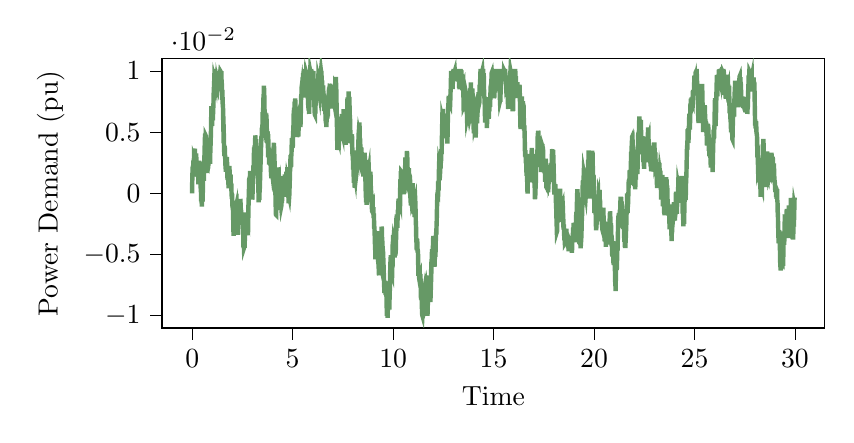
\begin{tikzpicture}

\definecolor{color0}{rgb}{0.12156862745098,0.466666666666667,0.705882352941177}

\definecolor{color0}{rgb}{1,0.498039215686275,0.0549019607843137}
\definecolor{color1}{rgb}{0.12156862745098,0.466666666666667,0.705882352941177}

\begin{axis}[
compat=newest,
tick align=outside,
tick pos=left,
x grid style={white!69.0196078431373!black},
xmin=-1.49950000000009, xmax=31.489500000002,
xtick style={color=black},
y grid style={white!69.0196078431373!black},
ymin=-0.011, ymax=0.011,
ytick style={color=black},
scaled y ticks=true,
%scaled y ticks=base 10:0,
width=10cm,
height=5cm,
xlabel=Time,
ylabel=Power Demand (pu),
%y label style={at={(-0.2,0.5)}}
]

\addplot [ultra thick, green!20!gray]
table {%
0 0
0 0.000797050554953481
0.01 0.00129835373411111
0.02 0.00218092303805788
0.03 0.00158612198449433
0.04 0.0015904349271483
0.05 0.00226136718906406
0.06 0.00253737171216475
0.07 0.00253791821554822
0.08 0.00199984021532999
0.09 0.00294611336621893
0.1 0.00290041044908807
0.11 0.00268940755291141
0.12 0.00337644445311739
0.13 0.00366406707836474
0.14 0.00302401211967498
0.15 0.00282990296187276
0.16 0.00250054994051814
0.17 0.0019875209906722
0.18 0.00229591017450012
0.19 0.00300326815262526
0.2 0.00326484840102321
0.21 0.00258923429584925
0.22 0.00196919756300523
0.23 0.00211450155458366
0.24 0.00137804664539079
0.25 0.00188481004777546
0.26 0.00151832599256504
0.27 0.00172898130344889
0.28 0.00133313488205297
0.29 0.00222953819369267
0.3 0.00137834171540657
0.31 0.000740824715719417
0.32 0.00167285772248945
0.33 0.0026498855067939
0.34 0.00201832602046733
0.35 0.00267399564176349
0.36 0.00236986373084894
0.37 0.00207561404159772
0.38 0.00229081582535605
0.39 0.00230025874098734
0.4 0.00193058799938833
0.41 0.00101494564246173
0.42 0.000547981761270382
0.43 0.000289871997477818
0.44 6.01063628089912e-05
0.45 -0.00065404305357231
0.46 0.000181277424123617
0.47 -0.000585639181601294
0.48 -0.00107397261824753
0.49 -0.000486397272923927
0.5 -0.000583509069419881
0.51 0.000166323884719516
0.52 -0.000659509344816852
0.53 0.000245732577936559
0.54 0.00119226431963124
0.55 0.00169483654666089
0.56 0.0013457600694775
0.57 0.00193708597850733
0.58 0.00103740735513626
0.59 0.00197736998929004
0.6 0.00227898887304026
0.61 0.002970631228984
0.62 0.00382839575478085
0.63 0.00401069801142619
0.64 0.00488706719929013
0.65 0.00453665968731789
0.66 0.00416043615493469
0.67 0.00472890750159033
0.68 0.00469350826826888
0.69 0.00384013434841858
0.7 0.00288244963732302
0.71 0.00287922790341886
0.72 0.00198139270124539
0.73 0.00188123257977627
0.74 0.00242972179505661
0.75 0.00167186070404365
0.76 0.00181771547004517
0.77 0.0027677740918702
0.78 0.00284339581968277
0.79 0.00205478382000541
0.8 0.0022746993560586
0.81 0.00272183829033199
0.820000000000001 0.00345895586449584
0.830000000000001 0.00417604314378269
0.840000000000001 0.00442425551567704
0.850000000000001 0.00376454986598559
0.860000000000001 0.00315202632934339
0.870000000000001 0.00299404203152899
0.880000000000001 0.00310083534856602
0.890000000000001 0.00242568933757506
0.900000000000001 0.00327491055619382
0.910000000000001 0.00353430341330592
0.920000000000001 0.00450895437008015
0.930000000000001 0.00461333266209304
0.940000000000001 0.00550898271679762
0.950000000000001 0.00648270305459712
0.960000000000001 0.00712911237998923
0.970000000000001 0.00625818113880963
0.980000000000001 0.00642332292664804
0.990000000000001 0.0055252316014222
1 0.0060829762071547
1.01 0.00660592318584863
1.02 0.00618997036693613
1.03 0.0059771762996601
1.04 0.00659377720798252
1.05 0.00696750764524617
1.06 0.00736915084090007
1.07 0.00811129531928032
1.08 0.0086024986155566
1.09 0.00880067166485348
1.1 0.00933487589660838
1.11 0.00926237957185105
1.12 0.00935790227243249
1.13 0.01
1.14 0.01
1.15 0.01
1.16 0.00925054521180424
1.17 0.01
1.18 0.00906469496939494
1.19 0.00907784678874062
1.2 0.00896955546772525
1.21 0.00919121127683083
1.22 0.00915003440340959
1.23 0.00940740246793738
1.24 0.00849608109122307
1.25 0.00909065041131265
1.26 0.00900644332617817
1.27 0.00928777757484961
1.28 0.00951013601316162
1.29 0.00881015687592976
1.3 0.00962702858195639
1.31 0.00990462511677266
1.32 0.00956914802072625
1.33 0.00923131325983269
1.34 0.00881102839333042
1.35 0.00932072605381783
1.36 0.00960501222210953
1.37 0.01
1.38 0.00972245439653673
1.39 0.00985472379366226
1.4 0.01
1.41 0.00997185151835699
1.42 0.00943203486389004
1.43 0.00945801234492065
1.44 0.00971646823958219
1.45 0.01
1.46 0.00916378908723297
1.47 0.00928695715096575
1.48 0.00847158931623383
1.49 0.00764632541341784
1.5 0.0084552816806248
1.51 0.00793474997751578
1.52 0.00729813408742686
1.53 0.00722516663565133
1.54 0.0063520808433017
1.55 0.00559640441346996
1.56 0.00567063203794435
1.57 0.00514453961251172
1.58 0.00440341770343518
1.59 0.00365453050643274
1.6 0.00305173186519543
1.61 0.00362730223159077
1.62 0.00387006979292214
1.63 0.00344728180209208
1.64 0.00289760673878372
1.65 0.00283530585469459
1.66 0.00198864264112255
1.67 0.00220787719990897
1.68 0.00176356513929741
1.69 0.00274167756845302
1.7 0.0022007001102598
1.71 0.00249781429599915
1.72 0.00267784443997871
1.73 0.00298770234837843
1.74 0.00212645482598465
1.75 0.00151469043827557
1.76 0.00109825571815567
1.77 0.00206181558098628
1.78 0.00149354496844318
1.79 0.00145102514525514
1.8 0.00118643516040512
1.81 0.000419037792272156
1.82 0.000783907902421753
1.83 0.00099183604600275
1.84 0.00153508646320931
1.85 0.00223814540500605
1.86 0.00191502371288427
1.87 0.00119577419782467
1.88 0.00133453803200528
1.89 0.000970135857977241
1.9 0.00145611524959405
1.91 0.00144019912670561
1.92 0.000630819519921621
1.93 0.00061666224114275
1.94 0.000840575963387059
1.95 0.000697863927513873
1.96 -0.000243956181899183
1.97 5.94385352241878e-05
1.98 -0.00046436316528189
1.99 -2.65103799758119e-05
2 -0.00090640983971398
2.01 -0.00118501951502731
2.02 -0.00105780357791968
2.03 -0.0013556643717365
2.04 -0.00197235423819081
2.05 -0.00284720787837215
2.06 -0.00347303585154025
2.07 -0.00297795316483718
2.08 -0.00246673070221153
2.09 -0.00150956326240845
2.1 -0.000907491843743666
2.11 -0.00119720252959024
2.12 -0.00137024988913652
2.13 -0.0011053699239044
2.14 -0.000821266507219873
2.15 -0.00148312512157782
2.16 -0.0015052881560925
2.17 -0.00114345443352567
2.18 -0.00107089840714287
2.19 -0.00198074902334148
2.2 -0.00101599947057496
2.21 -0.000970653168254504
2.22 -0.00175848029795422
2.23 -0.00150213815904063
2.24 -0.00086846513078384
2.25 -0.00169575876641606
2.26 -0.00244763066250706
2.27 -0.00337803736749003
2.28 -0.00277971057317859
2.29 -0.00186521127516979
2.29999999999999 -0.00159568190712025
2.30999999999999 -0.00150806955341451
2.31999999999999 -0.00118255256800894
2.32999999999999 -0.00183075289332628
2.33999999999999 -0.00145771624339694
2.34999999999999 -0.000844304837828456
2.35999999999999 -0.0016799313230913
2.36999999999999 -0.00141953042799279
2.37999999999999 -0.00186275578255281
2.38999999999999 -0.00141748120011655
2.39999999999999 -0.000442242307173367
2.40999999999999 -0.000890776959394735
2.41999999999999 -0.00136027603210555
2.42999999999999 -0.00123054471725617
2.43999999999999 -0.00200282273553097
2.44999999999999 -0.00236948404278743
2.45999999999999 -0.00250144521700542
2.46999999999999 -0.00176741117660364
2.47999999999999 -0.00160308356127261
2.48999999999999 -0.00231259178185071
2.49999999999999 -0.00243825681420243
2.50999999999999 -0.00208675445625488
2.51999999999999 -0.0028902118715711
2.52999999999999 -0.00251210699178259
2.53999999999999 -0.00334758279567096
2.54999999999999 -0.00329388056046008
2.55999999999999 -0.00387774993048085
2.56999999999999 -0.00386739928249641
2.57999999999999 -0.00443769183151439
2.58999999999999 -0.00438558366976021
2.59999999999999 -0.00373911751843251
2.60999999999999 -0.00445247135381489
2.61999999999999 -0.0037708454299003
2.62999999999999 -0.00296291804025126
2.63999999999999 -0.0021419347635158
2.64999999999999 -0.00155902072191523
2.65999999999999 -0.00248524318294872
2.66999999999999 -0.00326538359085353
2.67999999999999 -0.00292068996702378
2.68999999999999 -0.0023343954274624
2.69999999999999 -0.00285415107955303
2.70999999999999 -0.00341940874712585
2.71999999999999 -0.00267047588463217
2.72999999999999 -0.00320224180634589
2.73999999999999 -0.00243648802041156
2.74999999999999 -0.00338421275179076
2.75999999999999 -0.00327224146787558
2.76999999999998 -0.00273998019033455
2.77999999999998 -0.0021663886550153
2.78999999999998 -0.00222897317168078
2.79999999999998 -0.00129939743984138
2.80999999999998 -0.000631005161871845
2.81999999999998 0.000119452848080744
2.82999999999998 0.000470635288481179
2.83999999999998 0.00129018290871078
2.84999999999998 0.00113353877491491
2.85999999999998 0.000282555286896681
2.86999999999998 0.000850129510081967
2.87999999999998 0.00182924086335783
2.88999999999998 0.000910013452557035
2.89999999999998 0.000319639513284653
2.90999999999998 0.000109804860967462
2.91999999999998 0.00102427611870281
2.92999999999998 0.000647204071257488
2.93999999999998 2.69705013736602e-05
2.94999999999998 -9.3947934979793e-05
2.95999999999998 0.000320983803271864
2.96999999999998 5.02932761223614e-05
2.97999999999998 0.000235923596080933
2.98999999999998 -0.000493108519658644
2.99999999999998 -0.00040113499340045
3.00999999999998 0.000531018342086924
3.01999999999998 0.00113440988717724
3.02999999999998 0.000778570747295045
3.03999999999998 0.00131631780648846
3.04999999999998 0.00228871883797661
3.05999999999998 0.00187429197484931
3.06999999999998 0.0028525778635872
3.07999999999998 0.00376462564079154
3.08999999999998 0.00362760187002051
3.09999999999998 0.00311398659144982
3.10999999999998 0.0039266579140173
3.11999999999998 0.00312566145421104
3.12999999999998 0.00390241796606874
3.13999999999998 0.00474543415219548
3.14999999999998 0.00451515653857428
3.15999999999998 0.00406567156847626
3.16999999999998 0.00416554309257481
3.17999999999998 0.00442612364319187
3.18999999999998 0.0038887630958059
3.19999999999998 0.0035956292654937
3.20999999999998 0.00274895847925296
3.21999999999998 0.00320526128220508
3.22999999999998 0.00322970344482853
3.23999999999997 0.00266158188137992
3.24999999999997 0.00258177360853785
3.25999999999997 0.00297803561602365
3.26999999999997 0.0027447847936298
3.27999999999997 0.00181405815329794
3.28999999999997 0.000918529945065994
3.29999999999997 -2.06472534293534e-05
3.30999999999997 -0.000727370606381665
3.31999999999997 -0.000243064667467768
3.32999999999997 -1.86531717698406e-05
3.33999999999997 -0.000536325510892991
3.34999999999997 6.59504685346503e-05
3.35999999999997 0.00105980767501679
3.36999999999997 0.00126022444560095
3.37999999999997 0.00186198052104284
3.38999999999997 0.00177425668912995
3.39999999999997 0.00232523545168017
3.40999999999997 0.00261500445850547
3.41999999999997 0.00355002714240882
3.42999999999997 0.00384687241641749
3.43999999999997 0.00430745480798099
3.44999999999997 0.0047228343230545
3.45999999999997 0.0045511454298003
3.46999999999997 0.00538173533358345
3.47999999999997 0.00486819131332214
3.48999999999997 0.00525763146216836
3.49999999999997 0.00570847180134944
3.50999999999997 0.00663468343322078
3.51999999999997 0.00653983454361353
3.52999999999997 0.00685140408386442
3.53999999999997 0.00711927176870149
3.54999999999997 0.00801751617206216
3.55999999999997 0.00808318568078522
3.56999999999997 0.00879840102237901
3.57999999999997 0.00848432307438569
3.58999999999997 0.0079505331971827
3.59999999999997 0.00697669065949897
3.60999999999997 0.00603298903361617
3.61999999999997 0.0056960736949197
3.62999999999997 0.00544925661510217
3.63999999999997 0.00604804309390947
3.64999999999997 0.00659686514616247
3.65999999999997 0.00583642917986614
3.66999999999997 0.00516389279399666
3.67999999999997 0.00582071821355499
3.68999999999997 0.00487221920728724
3.69999999999997 0.00417834364808239
3.70999999999996 0.00477469641163698
3.71999999999996 0.00486242288949116
3.72999999999996 0.00422717617622731
3.73999999999996 0.00421633938597681
3.74999999999996 0.00507371428566933
3.75999999999996 0.00466995031972018
3.76999999999996 0.00387718640659108
3.77999999999996 0.00295006371411488
3.78999999999996 0.00370796665678044
3.79999999999996 0.00376193139461724
3.80999999999996 0.00323322189927548
3.81999999999996 0.00315396687817317
3.82999999999996 0.00236598979092993
3.83999999999996 0.00254261129652269
3.84999999999996 0.00294686777616916
3.85999999999996 0.00281390987210419
3.86999999999996 0.00284283975133481
3.87999999999996 0.00364453878607457
3.88999999999996 0.0035024236475845
3.89999999999996 0.00259411236660269
3.90999999999996 0.00274278631256752
3.91999999999996 0.00176661763166779
3.92999999999996 0.00152220144123695
3.93999999999996 0.00123167085987239
3.94999999999996 0.0015374906052374
3.95999999999996 0.00225703137900454
3.96999999999996 0.00138385286558906
3.97999999999996 0.00223655518115037
3.98999999999996 0.00129135719229373
3.99999999999996 0.00164104531252363
4.00999999999996 0.00128585294083857
4.01999999999996 0.0011474835289163
4.02999999999996 0.00121809164516357
4.03999999999996 0.00220940678438115
4.04999999999996 0.0030640655148482
4.05999999999996 0.00402061207290372
4.06999999999996 0.0041316853575302
4.07999999999996 0.00340125005146112
4.08999999999996 0.00309692979574654
4.09999999999996 0.00258557241876688
4.10999999999996 0.00188173380695228
4.11999999999996 0.00121228258835617
4.12999999999996 0.000751125620109862
4.13999999999996 0.000357874118876253
4.14999999999996 -0.000610788947708631
4.15999999999996 -0.00126498829559017
4.16999999999996 -0.00173687959408656
4.17999999999996 -0.00175388902976082
4.18999999999996 -0.000796578385719962
4.19999999999995 -0.000906102335955271
4.20999999999995 -0.00135290481048968
4.21999999999995 -0.00111012527571342
4.22999999999995 -0.000499964696318985
4.23999999999995 -0.000489847453501278
4.24999999999995 0.000487662987128391
4.25999999999995 0.00135719405723466
4.26999999999995 0.00119328423585139
4.27999999999995 0.0021323337026519
4.28999999999995 0.00172962910739143
4.29999999999995 0.00122035037299135
4.30999999999995 0.000636472340821989
4.31999999999995 0.000501692886114096
4.32999999999995 0.000597682545814451
4.33999999999995 0.000120662163432103
4.34999999999995 0.000723082417115186
4.35999999999995 0.000847774942487532
4.36999999999995 0.000819243866754514
4.37999999999995 -4.08252559924195e-05
4.38999999999995 -0.000255518932691301
4.39999999999995 -0.000319950491029283
4.40999999999995 -0.00122846129062634
4.41999999999995 -0.000893187669735662
4.42999999999995 -0.00108357993085905
4.43999999999995 -0.00100212026861453
4.44999999999995 -0.000317359338067748
4.45999999999995 -0.000512965321020004
4.46999999999995 -0.000793360018948529
4.47999999999995 0.000120501614114273
4.48999999999995 0.000635938192142555
4.49999999999995 0.00101786731359182
4.50999999999995 0.0014006886343885
4.51999999999995 0.000950801256087242
4.52999999999995 0.000171238663009207
4.53999999999995 0.00102506328275507
4.54999999999995 0.000179982036005294
4.55999999999995 -0.00027097081639188
4.56999999999995 0.000170208406367981
4.57999999999995 2.86264329211567e-05
4.58999999999995 -0.000227203716644701
4.59999999999995 0.000661728639226097
4.60999999999995 0.00155244579392334
4.61999999999995 0.000606288927085994
4.62999999999995 -0.000188163403760709
4.63999999999995 0.000320862071528473
4.64999999999995 0.000219568471570976
4.65999999999995 -0.000206627625340383
4.66999999999994 0.000409987308132296
4.67999999999994 0.000937183007090406
4.68999999999994 0.0017695326775588
4.69999999999994 0.00103675972242278
4.70999999999994 0.00108447376595142
4.71999999999994 0.00132030761653137
4.72999999999994 0.00124174057353221
4.73999999999994 0.00214936084852723
4.74999999999994 0.00137367899220536
4.75999999999994 0.000599075715978116
4.76999999999994 -0.000135544046919793
4.77999999999994 0.000727195821547855
4.78999999999994 -0.000225633430520081
4.79999999999994 -0.00080778044678755
4.80999999999994 -0.000214184836380045
4.81999999999994 -0.000169639289597723
4.82999999999994 -0.000248802728960095
4.83999999999994 -2.19749919482191e-05
4.84999999999994 0.000776636705217829
4.85999999999994 0.00112144630529577
4.86999999999994 0.00202253150024999
4.87999999999994 0.0017971255695277
4.88999999999994 0.00276844307605916
4.89999999999994 0.00314026400565671
4.90999999999994 0.00248059857674886
4.91999999999994 0.0021821215327667
4.92999999999994 0.00300394756355819
4.93999999999994 0.00317859331730357
4.94999999999994 0.00362326337978175
4.95999999999994 0.00451427664514392
4.96999999999994 0.00403029682035164
4.97999999999994 0.00449362246884152
4.98999999999994 0.00375542909309084
4.99999999999994 0.00411657251652882
5.00999999999994 0.00410100505642683
5.01999999999994 0.00500809054286573
5.02999999999994 0.00506762336788012
5.03999999999994 0.00548422405366455
5.04999999999994 0.00646452192785861
5.05999999999994 0.0065021803811014
5.06999999999994 0.00700914806840248
5.07999999999994 0.00628988027973265
5.08999999999994 0.00656248205626289
5.09999999999994 0.00748953589116205
5.10999999999994 0.00682585732770245
5.11999999999994 0.0074585658418016
5.12999999999994 0.0077623503582325
5.13999999999993 0.00689771358866251
5.14999999999993 0.00678291304588394
5.15999999999993 0.0070395290364713
5.16999999999993 0.00610744436456034
5.17999999999993 0.00617315802046376
5.18999999999993 0.00654536609100125
5.19999999999993 0.0061242847716979
5.20999999999993 0.00551236278427627
5.21999999999993 0.00459730896231619
5.22999999999993 0.00490919721190919
5.23999999999993 0.00511958775708643
5.24999999999993 0.00591960705577385
5.25999999999993 0.00508733124881024
5.26999999999993 0.00517903280895065
5.27999999999993 0.00465154544764332
5.28999999999993 0.00492482216548236
5.29999999999993 0.00557699125803689
5.30999999999993 0.00633143150874163
5.31999999999993 0.00634057011898255
5.32999999999993 0.00632357199388631
5.33999999999993 0.00683790359206816
5.34999999999993 0.00690473729651
5.35999999999993 0.00696971232770081
5.36999999999993 0.00641594515151169
5.37999999999993 0.00638292122599633
5.38999999999993 0.00542688246019456
5.39999999999993 0.00617978932015653
5.40999999999993 0.00687690953440406
5.41999999999993 0.00786411770811364
5.42999999999993 0.00803472119004053
5.43999999999993 0.00808352609124888
5.44999999999993 0.0087073117293499
5.45999999999993 0.0088354163943191
5.46999999999993 0.00862067007270918
5.47999999999993 0.00880540878401104
5.48999999999993 0.00910517135806917
5.49999999999993 0.00947746120276146
5.50999999999993 0.00936088337706932
5.51999999999993 0.00981763630842867
5.52999999999993 0.00929202783483689
5.53999999999993 0.00903890302652594
5.54999999999993 0.00812842155774838
5.55999999999993 0.00848217641317402
5.56999999999993 0.00863356600272061
5.57999999999993 0.00782728841326066
5.58999999999993 0.00871509555973332
5.59999999999993 0.00909415766832553
5.60999999999992 0.00999831651617863
5.61999999999992 0.01
5.62999999999992 0.00997758772232149
5.63999999999992 0.00961665333218406
5.64999999999992 0.01
5.65999999999992 0.00940359463123547
5.66999999999992 0.00988933768718676
5.67999999999992 0.00983143663408567
5.68999999999992 0.01
5.69999999999992 0.00914050795273828
5.70999999999992 0.00892251996788498
5.71999999999992 0.00907468382351556
5.72999999999992 0.009198277120269
5.73999999999992 0.00883085160944519
5.74999999999992 0.00832282764883244
5.75999999999992 0.00790827012746356
5.76999999999992 0.00721637050831619
5.77999999999992 0.00747536889064798
5.78999999999992 0.00678073923191539
5.79999999999992 0.00711249762144192
5.80999999999992 0.00685714260968384
5.81999999999992 0.00649781255539029
5.82999999999992 0.00716297545210819
5.83999999999992 0.00789751434357324
5.84999999999992 0.00879779856663711
5.85999999999992 0.00895481588000236
5.86999999999992 0.00913656859347702
5.87999999999992 0.00993427737417066
5.88999999999992 0.00984696822873284
5.89999999999992 0.00937807529485991
5.90999999999992 0.00949426332897429
5.91999999999992 0.01
5.92999999999992 0.01
5.93999999999992 0.00959302814204044
5.94999999999992 0.00989565810658165
5.95999999999992 0.01
5.96999999999992 0.00951744795854232
5.97999999999992 0.00878223548727128
5.98999999999992 0.00966243585660478
5.99999999999992 0.01
6.00999999999992 0.00941951520477788
6.01999999999992 0.00963306505549131
6.02999999999992 0.01
6.03999999999992 0.00902319781350604
6.04999999999992 0.00903210715289929
6.05999999999992 0.00829816317913744
6.06999999999992 0.00788691643052785
6.07999999999991 0.00712488384785184
6.08999999999991 0.00704574858036663
6.09999999999991 0.00646736645532871
6.10999999999991 0.00643151776550018
6.11999999999991 0.00726420133613505
6.12999999999991 0.00653390740117736
6.13999999999991 0.00721899308148941
6.14999999999991 0.00818949429841118
6.15999999999991 0.00890129048478628
6.16999999999991 0.00919358616576949
6.17999999999991 0.00885385460419851
6.18999999999991 0.00937951692148907
6.19999999999991 0.00900062983256524
6.20999999999991 0.00845850009134261
6.21999999999991 0.0075426324278322
6.22999999999991 0.00835628376386359
6.23999999999991 0.00910302759215987
6.24999999999991 0.00914582788175688
6.25999999999991 0.00821169468609759
6.26999999999991 0.00854246228523273
6.27999999999991 0.00937210237820059
6.28999999999991 0.00929539093346878
6.29999999999991 0.00944738171216187
6.30999999999991 0.00900881878490283
6.31999999999991 0.00900091580157923
6.32999999999991 0.00817261460545501
6.33999999999991 0.00805991989712984
6.34999999999991 0.00832025228556928
6.35999999999991 0.00766954710382112
6.36999999999991 0.00840537390280862
6.37999999999991 0.00902787964982955
6.38999999999991 0.00998713939427945
6.39999999999991 0.00982694598067635
6.40999999999991 0.01
6.41999999999991 0.00986415500074349
6.42999999999991 0.01
6.43999999999991 0.00952607377459324
6.44999999999991 0.00909769769185116
6.45999999999991 0.00895132854883622
6.46999999999991 0.00922735904796591
6.47999999999991 0.00829256337082411
6.48999999999991 0.00863878307943384
6.49999999999991 0.00800864368617774
6.50999999999991 0.00870631099069982
6.51999999999991 0.00882657947480825
6.52999999999991 0.0079380533495192
6.53999999999991 0.00769865538627404
6.5499999999999 0.00759495211757747
6.5599999999999 0.00697962535162511
6.5699999999999 0.00674177798066165
6.5799999999999 0.00747494942859258
6.5899999999999 0.00753938707159552
6.5999999999999 0.00750927089539499
6.6099999999999 0.00771064313986109
6.6199999999999 0.00718580951530194
6.6299999999999 0.00724875448510753
6.6399999999999 0.00713845136393084
6.6499999999999 0.00625276324036495
6.6599999999999 0.00569229818226695
6.6699999999999 0.00593083734114517
6.6799999999999 0.00542539374774822
6.6899999999999 0.00603645895145258
6.6999999999999 0.00672304434841372
6.7099999999999 0.0067346589255884
6.7199999999999 0.00699727320920372
6.7299999999999 0.00611959669317734
6.7399999999999 0.00708986158407487
6.7499999999999 0.00630170509067489
6.7599999999999 0.00728158966565879
6.7699999999999 0.00691112245697558
6.7799999999999 0.00790746760670076
6.7899999999999 0.00756137924167532
6.7999999999999 0.007906999749901
6.8099999999999 0.00865419012510775
6.8199999999999 0.00788096379864036
6.8299999999999 0.00835178150947276
6.8399999999999 0.00861882279211744
6.8499999999999 0.00897641140213478
6.8599999999999 0.00804591741286458
6.8699999999999 0.00818955324303884
6.8799999999999 0.00784563224801112
6.8899999999999 0.00830427058262393
6.8999999999999 0.00832937597580617
6.9099999999999 0.00750691007911725
6.9199999999999 0.00765442379058977
6.9299999999999 0.00830652359404281
6.9399999999999 0.00749843027139749
6.9499999999999 0.00766048150014662
6.9599999999999 0.00714159929128842
6.9699999999999 0.00694519776760909
6.9799999999999 0.00750387609974232
6.9899999999999 0.00843793748022488
6.9999999999999 0.00841333123952953
7.00999999999989 0.00819394704679263
7.01999999999989 0.00882801121368059
7.02999999999989 0.00797381914180975
7.03999999999989 0.00701200551414511
7.04999999999989 0.00773841322247232
7.05999999999989 0.00751453545284854
7.06999999999989 0.00741475007317148
7.07999999999989 0.00759899519711493
7.08999999999989 0.00801108616772877
7.09999999999989 0.00798543541876466
7.10999999999989 0.00846789805115732
7.11999999999989 0.00905400943428494
7.12999999999989 0.00902876061764851
7.13999999999989 0.00922399320577853
7.14999999999989 0.00951273129423254
7.15999999999989 0.00901409591604996
7.16999999999989 0.00865853273148875
7.17999999999989 0.00783494897230583
7.18999999999989 0.00685623863540921
7.19999999999989 0.00599684086691045
7.20999999999989 0.00503625898169468
7.21999999999989 0.00414634219327717
7.22999999999989 0.00355875601439274
7.23999999999989 0.0039566669562127
7.24999999999989 0.00472557108227181
7.25999999999989 0.00432979766070252
7.26999999999989 0.0041206085988392
7.27999999999989 0.00385534129103886
7.28999999999989 0.00354718880082918
7.29999999999989 0.00438173360756623
7.30999999999989 0.00431538878711466
7.31999999999989 0.00460531207574546
7.32999999999989 0.00546355985136529
7.33999999999989 0.00457746945397353
7.34999999999989 0.00515136393486501
7.35999999999989 0.00451198363603806
7.36999999999989 0.00526982722022096
7.37999999999989 0.00500907120026362
7.38999999999989 0.00544129312613105
7.39999999999989 0.00562894867702113
7.40999999999989 0.00615061843588683
7.41999999999989 0.00624505686572101
7.42999999999989 0.00557743517489584
7.43999999999989 0.00599422944865003
7.44999999999989 0.00648511739700187
7.45999999999989 0.00563542546288618
7.46999999999989 0.00489343644140998
7.47999999999988 0.00482425907639734
7.48999999999988 0.00558683718287582
7.49999999999988 0.00542083083631675
7.50999999999988 0.00584765099990401
7.51999999999988 0.00507966181609259
7.52999999999988 0.00592876415664633
7.53999999999988 0.00688804671513322
7.54999999999988 0.00656001327593028
7.55999999999988 0.00560442747601453
7.56999999999988 0.00560604472821487
7.57999999999988 0.00588176942504018
7.58999999999988 0.00637369575537596
7.59999999999988 0.00568438342504491
7.60999999999988 0.00481029012683205
7.61999999999988 0.0049774906769008
7.62999999999988 0.00434729414278767
7.63999999999988 0.00397510361557363
7.64999999999988 0.00431180402942965
7.65999999999988 0.00526216214681245
7.66999999999988 0.00583998057267689
7.67999999999988 0.00600227342529747
7.68999999999988 0.00554704770842708
7.69999999999988 0.00560814479433642
7.70999999999988 0.00642068930054971
7.71999999999988 0.007043875694992
7.72999999999988 0.00784684174311129
7.73999999999988 0.00754669908974783
7.74999999999988 0.00697710016393912
7.75999999999988 0.00764327937430523
7.76999999999988 0.00691114613470955
7.77999999999988 0.00750739410816142
7.78999999999988 0.00833746723029789
7.79999999999988 0.00744005052394671
7.80999999999988 0.00766105303030744
7.81999999999988 0.00785793632250576
7.82999999999988 0.00727422330304206
7.83999999999988 0.00648948285356525
7.84999999999988 0.00621731332755968
7.85999999999988 0.00600332909935018
7.86999999999988 0.0050568890647444
7.87999999999988 0.00408435026221025
7.88999999999988 0.00474866128621105
7.89999999999988 0.0046706756233159
7.90999999999988 0.00461081980336977
7.91999999999988 0.0045129888763065
7.92999999999988 0.00466642331500281
7.93999999999988 0.00482714379177854
7.94999999999987 0.00432245249507585
7.95999999999987 0.00434507504839922
7.96999999999987 0.00361060683181533
7.97999999999987 0.00304564452523691
7.98999999999987 0.00314553686875002
7.99999999999987 0.00287924258312923
8.00999999999987 0.00195549738814968
8.01999999999987 0.00233124060991765
8.02999999999987 0.00181403681908371
8.03999999999987 0.00134391350377051
8.04999999999987 0.000857297746782564
8.05999999999987 0.00133006393913309
8.06999999999987 0.00102979114711426
8.07999999999987 0.00121848310172372
8.08999999999987 0.000454952408164714
8.09999999999987 0.000635321366965838
8.10999999999987 0.0013893535781488
8.11999999999987 0.001279809450561
8.12999999999987 0.00154925934740208
8.13999999999987 0.00238337576771814
8.14999999999987 0.00334379433846965
8.15999999999987 0.00239029169738525
8.16999999999987 0.0030371428784381
8.17999999999987 0.00350799489563788
8.18999999999987 0.00289460933514234
8.19999999999987 0.00306561265288148
8.20999999999987 0.00241665328941831
8.21999999999987 0.00258648938835088
8.22999999999987 0.00237947341928667
8.23999999999987 0.00251434477031038
8.24999999999987 0.00289129313498153
8.25999999999987 0.00370520382318319
8.26999999999987 0.00390832674321256
8.27999999999987 0.00476027629232201
8.28999999999987 0.00497573366031675
8.29999999999987 0.00489450416733598
8.30999999999987 0.00545718670917048
8.31999999999987 0.005788824987981
8.32999999999987 0.00547577160042766
8.33999999999987 0.00469648359242684
8.34999999999987 0.00373147980316034
8.35999999999987 0.00446849265142461
8.36999999999987 0.00373575943609387
8.37999999999987 0.00304053697527742
8.38999999999987 0.00377162921020565
8.39999999999987 0.00362813706553696
8.40999999999987 0.00348231256395849
8.41999999999986 0.00342566745112218
8.42999999999986 0.00258163846697636
8.43999999999986 0.00263608636206483
8.44999999999986 0.00199576347148775
8.45999999999986 0.00224254231997179
8.46999999999986 0.00187381122774938
8.47999999999986 0.00221198401700346
8.48999999999986 0.00235206219446936
8.49999999999986 0.00310665679088085
8.50999999999986 0.00234552244956471
8.51999999999986 0.00137176434079739
8.52999999999986 0.00221783993039155
8.53999999999986 0.00215140574768986
8.54999999999986 0.00191438067521065
8.55999999999986 0.00192310390581757
8.56999999999986 0.00266723460500181
8.57999999999986 0.00331810668828653
8.58999999999986 0.00308086715214141
8.59999999999986 0.00221227991557666
8.60999999999986 0.0019731511134514
8.61999999999986 0.00128675994222329
8.62999999999986 0.000546531917888213
8.63999999999986 1.11686277224368e-05
8.64999999999986 -0.000379599515993709
8.65999999999986 -0.000367567462223252
8.66999999999986 -0.000401925021601217
8.67999999999986 -0.000926331110240423
8.68999999999986 -4.91178830107576e-05
8.69999999999986 -8.85904199548265e-05
8.70999999999986 -0.000703222988689294
8.71999999999986 8.18626181396246e-05
8.72999999999986 0.00037148799432345
8.73999999999986 0.000979845784029214
8.74999999999986 0.00150155000683592
8.75999999999986 0.0019702736416643
8.76999999999986 0.00273721382467505
8.77999999999986 0.00183989440619548
8.78999999999986 0.00193859468038835
8.79999999999986 0.00147731020482278
8.80999999999986 0.00127805633742843
8.81999999999986 0.000915912149706798
8.82999999999986 0.00108262273069267
8.83999999999986 0.00089203080972234
8.84999999999986 0.000555985293692047
8.85999999999986 0.00127658535786129
8.86999999999986 0.00177664819795108
8.87999999999986 0.00137892405680193
8.88999999999985 0.000531757413679279
8.89999999999985 0.000267238968913193
8.90999999999985 -6.82291536733814e-05
8.91999999999985 -0.000322664321942988
8.92999999999985 -0.000770239961857428
8.93999999999985 -0.000862916029876027
8.94999999999985 -0.00142508885901315
8.95999999999985 -0.00146126138823857
8.96999999999985 -0.000538926522013817
8.97999999999985 -0.000516858147018557
8.98999999999985 -0.0014519465453722
8.99999999999985 -0.00115296252595501
9.00999999999985 -0.0014418900668091
9.01999999999985 -0.00111700852704902
9.02999999999985 -0.00202591290352538
9.03999999999985 -0.00163253737037506
9.04999999999985 -0.00216711110503656
9.05999999999985 -0.00288512041380141
9.06999999999985 -0.00269830526033164
9.07999999999985 -0.0032706500724616
9.08999999999985 -0.00365641183143108
9.09999999999985 -0.00435368162137988
9.10999999999985 -0.00466095536811554
9.11999999999985 -0.00538180283423214
9.12999999999985 -0.0051039313103072
9.13999999999985 -0.00476283527723736
9.14999999999985 -0.00426084099620969
9.15999999999985 -0.0043897489928486
9.16999999999985 -0.00378175722121455
9.17999999999985 -0.00460325005821057
9.18999999999985 -0.00424610333610931
9.19999999999985 -0.00361816441915733
9.20999999999985 -0.0033196256136871
9.21999999999985 -0.00308836501979506
9.22999999999985 -0.00382561224828572
9.23999999999985 -0.00446392965578422
9.24999999999985 -0.00542904385014942
9.25999999999985 -0.00561568849114545
9.26999999999985 -0.00575301620187197
9.27999999999985 -0.00592072432982704
9.28999999999985 -0.00653735089671705
9.29999999999985 -0.0066944885127787
9.30999999999985 -0.00596841033835791
9.31999999999985 -0.00530963591082935
9.32999999999985 -0.00534227131920117
9.33999999999985 -0.00564866005956979
9.34999999999985 -0.00567531183959106
9.35999999999984 -0.00542320826920334
9.36999999999984 -0.00569411840874118
9.37999999999984 -0.00577669938046351
9.38999999999984 -0.00484612865593622
9.39999999999984 -0.00535777179955122
9.40999999999984 -0.00443109411197552
9.41999999999984 -0.0035056398075564
9.42999999999984 -0.00271586326689766
9.43999999999984 -0.00285058280664464
9.44999999999984 -0.00367823335876409
9.45999999999984 -0.00383463346167726
9.46999999999984 -0.00424919353380173
9.47999999999984 -0.00440702316006672
9.48999999999984 -0.00490951805725762
9.49999999999984 -0.00542623718810881
9.50999999999984 -0.00574306241653704
9.51999999999984 -0.00568683432869752
9.52999999999984 -0.00611779693838453
9.53999999999984 -0.00677735809072926
9.54999999999984 -0.00711953834076248
9.55999999999984 -0.00789002462023195
9.56999999999984 -0.00814292556893061
9.57999999999984 -0.00725570305163683
9.58999999999984 -0.0074786873431571
9.59999999999984 -0.00805437054616849
9.60999999999984 -0.00714903081420981
9.61999999999984 -0.00795934141494726
9.62999999999984 -0.00829656736146147
9.63999999999984 -0.00737516016734148
9.64999999999984 -0.00801064748961502
9.65999999999984 -0.00842049605021157
9.66999999999984 -0.00830199193252364
9.67999999999984 -0.00924780350273247
9.68999999999984 -0.01
9.69999999999984 -0.00947016499402126
9.70999999999984 -0.0093995133805741
9.71999999999984 -0.01
9.72999999999984 -0.01
9.73999999999984 -0.00918561907137025
9.74999999999984 -0.00895794263902539
9.75999999999984 -0.00823132333336061
9.76999999999984 -0.00790584919670402
9.77999999999984 -0.00830432716073549
9.78999999999984 -0.00799139908311996
9.79999999999984 -0.00864305753902881
9.80999999999984 -0.00949766075972865
9.81999999999984 -0.00879097481482978
9.82999999999983 -0.0082954917802704
9.83999999999983 -0.00755556649576346
9.84999999999983 -0.00656715473343238
9.85999999999983 -0.00611144643152147
9.86999999999983 -0.00549022953489285
9.87999999999983 -0.00522657959215593
9.88999999999983 -0.00506050691964054
9.89999999999983 -0.00592370413367995
9.90999999999983 -0.0063368488990083
9.91999999999983 -0.00576186982623277
9.92999999999983 -0.00563704149549047
9.93999999999983 -0.00660899782040096
9.94999999999983 -0.00666009777822053
9.95999999999983 -0.00595302667148222
9.96999999999983 -0.00507370162341188
9.97999999999983 -0.00511708225949169
9.98999999999983 -0.00412933027541371
9.99999999999983 -0.00341470998901971
10.0099999999998 -0.00383363006266473
10.0199999999998 -0.0038174453608699
10.0299999999998 -0.00358743763107014
10.0399999999998 -0.00365275186306861
10.0499999999998 -0.0042041040506704
10.0599999999998 -0.00380525210438938
10.0699999999998 -0.00455008917129789
10.0799999999998 -0.00525316248528542
10.0899999999998 -0.00460051721382953
10.0999999999998 -0.00484214827586529
10.1099999999998 -0.00507069947310698
10.1199999999998 -0.00442168334231336
10.1299999999998 -0.00492174644521258
10.1399999999998 -0.00408415974670733
10.1499999999998 -0.00351710658232615
10.1599999999998 -0.00262676213177007
10.1699999999998 -0.00265986323620432
10.1799999999998 -0.00232050260126187
10.1899999999998 -0.00171478682020236
10.1999999999998 -0.00198676825241578
10.2099999999998 -0.00280285284459845
10.2199999999998 -0.00220139892044037
10.2299999999998 -0.00206413739467479
10.2399999999998 -0.00133156738192222
10.2499999999998 -0.00173586903279521
10.2599999999998 -0.000921856651281745
10.2699999999998 -0.000437278865328332
10.2799999999998 -0.00083944971039048
10.2899999999998 -0.00131737751632753
10.2999999999998 -0.00144458275784921
10.3099999999998 -0.000815831068923606
10.3199999999998 -0.000706026081271872
10.3299999999998 -0.00113332289338819
10.3399999999998 -0.000449057187162161
10.3499999999998 -0.000529590993981636
10.3599999999998 0.00040108259419889
10.3699999999998 0.000684425364462068
10.3799999999998 0.00125417018563205
10.3899999999998 0.00181437121727876
10.3999999999998 0.000927722891519437
10.4099999999998 0.00177043492739218
10.4199999999998 0.00174751054389299
10.4299999999998 0.000870998963625024
10.4399999999998 0.00110559987415313
10.4499999999998 0.000187956386175218
10.4599999999998 0.00108143538552014
10.4699999999998 0.000878930084769761
10.4799999999998 0.000947979038106052
10.4899999999998 0.00125949834347441
10.4999999999998 0.000291041102909163
10.5099999999998 0.000554919740300423
10.5199999999998 0.00065747795606401
10.5299999999998 -7.89990130936409e-05
10.5399999999998 0.000338661993370188
10.5499999999998 0.000414149642435356
10.5599999999998 3.48288877331599e-05
10.5699999999998 0.000709900015078743
10.5799999999998 0.000984881349991168
10.5899999999998 0.0015548883194343
10.5999999999998 0.00209379311782931
10.6099999999998 0.00294417060179
10.6199999999998 0.0024971153591031
10.6299999999998 0.00205765520497329
10.6399999999998 0.00176461130853004
10.6499999999998 0.00127714048622033
10.6599999999998 0.00121071259767941
10.6699999999998 0.00211768689542194
10.6799999999998 0.00269765196801396
10.6899999999998 0.00347784146830287
10.6999999999998 0.00306407954559089
10.7099999999998 0.00283921914113279
10.7199999999998 0.00195010617197151
10.7299999999998 0.00146706306800272
10.7399999999998 0.00129479767247863
10.7499999999998 0.00102840543573332
10.7599999999998 0.000595239323953049
10.7699999999998 0.00145039727104003
10.7799999999998 0.00206822986746293
10.7899999999998 0.00109929412921766
10.7999999999998 0.00131776384066649
10.8099999999998 0.00158650882211411
10.8199999999998 0.000846526155684073
10.8299999999998 0.00140634153063303
10.8399999999998 0.0013551460698647
10.8499999999998 0.000367314433571523
10.8599999999998 -0.000252316567452679
10.8699999999998 -0.000590504668767659
10.8799999999998 -0.000848078970844443
10.8899999999998 -0.000978329209082655
10.8999999999998 -0.000143936225911746
10.9099999999998 -0.000248734714906507
10.9199999999998 -0.00047404042175035
10.9299999999998 -0.000385433657976894
10.9399999999998 -0.000371847418604644
10.9499999999998 -6.34458126892977e-05
10.9599999999998 0.000473552131975693
10.9699999999998 0.00083903858929839
10.9799999999998 0.000268795633831479
10.9899999999998 -0.000590990525144894
10.9999999999998 -0.00114539497835266
11.0099999999998 -0.00157484145523037
11.0199999999998 -0.00104226952736816
11.0299999999998 -0.00169783053489913
11.0399999999998 -0.00085136827738835
11.0499999999998 -0.0012685129394566
11.0599999999998 -0.00150476226247801
11.0699999999998 -0.00192370965499538
11.0799999999998 -0.00114265779187066
11.0899999999998 -0.000585403385869908
11.0999999999998 -0.000509921127138454
11.1099999999998 -0.000876091496176683
11.1199999999998 -0.00153472661266872
11.1299999999998 -0.00240160692494641
11.1399999999998 -0.00265119172561323
11.1499999999998 -0.00355027637801546
11.1599999999998 -0.00385906153504993
11.1699999999998 -0.00451598833716997
11.1799999999998 -0.00462621551847924
11.1899999999998 -0.00371671078715664
11.1999999999998 -0.00382513551290765
11.2099999999998 -0.00419457436713745
11.2199999999998 -0.00480452310226945
11.2299999999998 -0.00466581703058118
11.2399999999998 -0.00493052896908704
11.2499999999998 -0.0059226095072676
11.2599999999998 -0.00673245555581893
11.2699999999998 -0.00622128069353769
11.2799999999998 -0.00623732225945101
11.2899999999998 -0.00677853810881224
11.2999999999998 -0.00697168531113328
11.3099999999998 -0.00707142648424479
11.3199999999998 -0.00684265809309942
11.3299999999998 -0.00678616282886856
11.3399999999998 -0.00749508714048747
11.3499999999998 -0.00720352618593432
11.3599999999998 -0.00657982889972136
11.3699999999998 -0.00737695571177847
11.3799999999998 -0.00824923413502618
11.3899999999998 -0.00868061440652832
11.3999999999998 -0.00844739423072542
11.4099999999998 -0.00823686894803173
11.4199999999998 -0.00855964686625378
11.4299999999998 -0.00910137383019814
11.4399999999998 -0.00968110710677886
11.4499999999998 -0.00994318591706588
11.4599999999998 -0.01
11.4699999999998 -0.00970264292674052
11.4799999999998 -0.01
11.4899999999998 -0.01
11.4999999999998 -0.00994194772246693
11.5099999999998 -0.00941556812490967
11.5199999999998 -0.00844735895198828
11.5299999999998 -0.00817004033658826
11.5399999999998 -0.00803962950995726
11.5499999999998 -0.00793530245645357
11.5599999999998 -0.00815670258781681
11.5699999999998 -0.00802752959545653
11.5799999999998 -0.00840695457777327
11.5899999999998 -0.0078596271923262
11.5999999999998 -0.00777261833926159
11.6099999999998 -0.00812500392002299
11.6199999999998 -0.00835429953432945
11.6299999999998 -0.00845520663647867
11.6399999999998 -0.00881259176767643
11.6499999999998 -0.00963330770191116
11.6599999999998 -0.00966630813964911
11.6699999999998 -0.01
11.6799999999998 -0.00954180787521194
11.6899999999998 -0.00906448742462544
11.6999999999998 -0.00974821423904869
11.7099999999998 -0.01
11.7199999999998 -0.00958155145444734
11.7299999999998 -0.00881399024296237
11.7399999999998 -0.00839704980002093
11.7499999999998 -0.00816731089041051
11.7599999999998 -0.007345241092767
11.7699999999998 -0.00700460765642694
11.7799999999998 -0.00694236516165565
11.7899999999998 -0.00695121678571015
11.7999999999998 -0.00760767538226573
11.8099999999998 -0.00814359019415526
11.8199999999998 -0.00745351784901134
11.8299999999998 -0.00794847103498631
11.8399999999998 -0.00819195598721341
11.8499999999998 -0.00888108133988843
11.8599999999998 -0.00825487442096731
11.8699999999998 -0.00748451689878142
11.8799999999998 -0.00699751049343162
11.8899999999998 -0.00708392545132962
11.8999999999998 -0.0065518238749984
11.9099999999998 -0.00612245127696731
11.9199999999998 -0.00548745294188072
11.9299999999998 -0.00494405405680046
11.9399999999998 -0.00457073965295658
11.9499999999998 -0.00520075137600408
11.9599999999998 -0.00555392134699414
11.9699999999998 -0.00483300569551716
11.9799999999998 -0.00451269935539951
11.9899999999998 -0.00378368833899647
11.9999999999998 -0.00348580607203759
12.0099999999998 -0.00407644165587386
12.0199999999998 -0.00402642098702759
12.0299999999998 -0.0047932291424507
12.0399999999998 -0.00503358058370678
12.0499999999998 -0.0054111375853613
12.0599999999998 -0.00599214456686207
12.0699999999998 -0.00561325791092306
12.0799999999998 -0.00503688057408122
12.0899999999998 -0.00448466227314933
12.0999999999998 -0.00516560283350837
12.1099999999998 -0.00490934248572956
12.1199999999998 -0.00403505017731171
12.1299999999998 -0.00367931653217481
12.1399999999998 -0.00319951664530426
12.1499999999998 -0.00333690141915437
12.1599999999998 -0.00271689683943439
12.1699999999998 -0.00227596739569807
12.1799999999998 -0.0014892968974374
12.1899999999998 -0.000724424431255367
12.1999999999998 -0.00033813474336756
12.2099999999998 0.000108615774911904
12.2199999999998 -0.000551830135601474
12.2299999999998 0.000143954785844798
12.2399999999998 0.00010547306574098
12.2499999999998 0.000972581878497048
12.2599999999998 0.000208143369858894
12.2699999999998 0.00109213429680381
12.2799999999998 0.00185589540547335
12.2899999999998 0.00238026904671923
12.2999999999998 0.00230216189754804
12.3099999999998 0.0017518114228407
12.3199999999998 0.00106785044702956
12.3299999999998 0.00184271010301576
12.3399999999998 0.00161373525411194
12.3499999999998 0.00236760962019321
12.3599999999998 0.0020375102674461
12.3699999999998 0.00245042232178273
12.3799999999998 0.00257156386863718
12.3899999999998 0.00274957039066308
12.3999999999998 0.00361716341206147
12.4099999999998 0.00321453118175886
12.4199999999998 0.00367756966297314
12.4299999999998 0.00463238566382166
12.4399999999998 0.00538701174160184
12.4499999999998 0.00615415346970979
12.4599999999998 0.00608329326887965
12.4699999999998 0.00633660173923552
12.4799999999998 0.00691366471759673
12.4899999999998 0.00603520448610094
12.4999999999998 0.00616251757769243
12.5099999999998 0.00642822618944353
12.5199999999998 0.00612332705974647
12.5299999999998 0.00522256014076769
12.5399999999998 0.00565137187422647
12.5499999999998 0.00599030971507746
12.5599999999998 0.00647147885489383
12.5699999999998 0.00618881773526211
12.5799999999998 0.00581354850096878
12.5899999999998 0.00518219780526387
12.5999999999998 0.00449737562806255
12.6099999999998 0.00537513643857683
12.6199999999998 0.00471358329657266
12.6299999999998 0.00457431625141622
12.6399999999998 0.00495577042365098
12.6499999999998 0.00521234877994226
12.6599999999998 0.00463975581517402
12.6699999999998 0.00562768597837748
12.6799999999998 0.0051763182430652
12.6899999999998 0.00502586780661008
12.6999999999998 0.00407867044842368
12.7099999999998 0.0047264745651815
12.7199999999998 0.0057064056033286
12.7299999999998 0.00658133348307809
12.7399999999998 0.00702499537843454
12.7499999999998 0.00712775493949485
12.7599999999998 0.0076502531500614
12.7699999999998 0.00797381658467306
12.7799999999998 0.00718100861157368
12.7899999999998 0.00780381401678481
12.7999999999998 0.00730494961312497
12.8099999999998 0.0074883225218698
12.8199999999998 0.00723752491412475
12.8299999999998 0.00741807700845413
12.8399999999998 0.00737206066908985
12.8499999999998 0.00781973907211511
12.8599999999998 0.00840156064736405
12.8699999999998 0.00856992987140043
12.8799999999998 0.00949138195161281
12.8899999999998 0.01
12.8999999999998 0.00987826307938471
12.9099999999998 0.00968211200661147
12.9199999999998 0.00918749409794859
12.9299999999998 0.00999410645984756
12.9399999999998 0.0094076464447357
12.9499999999998 0.00873711429206956
12.9599999999998 0.00852772187280677
12.9699999999998 0.0089771634845963
12.9799999999998 0.00920012648809724
12.9899999999998 0.00979846491154788
12.9999999999998 0.01
13.0099999999998 0.01
13.0199999999998 0.00957144023313842
13.0299999999998 0.00995466321826878
13.0399999999998 0.01
13.0499999999998 0.01
13.0599999999998 0.00994508270348161
13.0699999999998 0.01
13.0799999999998 0.00974844196163148
13.0899999999998 0.00974760851467989
13.0999999999998 0.01
13.1099999999998 0.01
13.1199999999998 0.00946730053087429
13.1299999999998 0.00983236432344184
13.1399999999998 0.00970010363270351
13.1499999999998 0.00959670733046084
13.1599999999998 0.01
13.1699999999998 0.01
13.1799999999998 0.00951519373194284
13.1899999999998 0.00963648854970066
13.1999999999998 0.0091897194742803
13.2099999999998 0.00957189972012796
13.2199999999998 0.01
13.2299999999998 0.01
13.2399999999998 0.00914509758452282
13.2499999999998 0.00980654746280761
13.2599999999998 0.00950340732534517
13.2699999999998 0.00969797435546022
13.2799999999998 0.00920018348052332
13.2899999999998 0.00861054753259741
13.2999999999998 0.00925176047204647
13.3099999999998 0.0085022229448069
13.3199999999998 0.00936102727725012
13.3299999999998 0.00989187066026249
13.3399999999998 0.01
13.3499999999998 0.01
13.3599999999998 0.00972069474928595
13.3699999999998 0.01
13.3799999999998 0.01
13.3899999999998 0.01
13.3999999999998 0.00997800129981001
13.4099999999998 0.00954298147823083
13.4199999999998 0.00875967010294266
13.4299999999998 0.00851948733207869
13.4399999999998 0.00869743869496034
13.4499999999998 0.00843851508698202
13.4599999999998 0.00897976883331532
13.4699999999998 0.00872867917088264
13.4799999999998 0.00890173364938815
13.4899999999998 0.00894623118327453
13.4999999999998 0.00796564032552106
13.5099999999998 0.00709389617146672
13.5199999999998 0.00713171839571258
13.5299999999998 0.00758044095757272
13.5399999999998 0.0078875086835954
13.5499999999998 0.00766113073422597
13.5599999999998 0.00755726170963701
13.5699999999998 0.00735939187867823
13.5799999999998 0.00814101634593895
13.5899999999998 0.0084320217173019
13.5999999999998 0.00797305732064602
13.6099999999998 0.00775021838348708
13.6199999999998 0.00781402417040891
13.6299999999998 0.00815827492926469
13.6399999999998 0.00807503484601079
13.6499999999998 0.00759380781312213
13.6599999999998 0.00696684902960439
13.6699999999998 0.00681452565382143
13.6799999999998 0.0062014475332119
13.6899999999998 0.00628677130850798
13.6999999999998 0.0065939822972555
13.7099999999998 0.0069043816186294
13.7199999999998 0.00692104901928415
13.7299999999998 0.00716942281058273
13.7399999999998 0.00618061155885176
13.7499999999998 0.0070541941291643
13.7599999999998 0.00665140865940749
13.7699999999998 0.00574404779608107
13.7799999999998 0.0060302144037401
13.7899999999998 0.0062120698833645
13.7999999999998 0.00609589476242606
13.8099999999998 0.00617429564872735
13.8199999999997 0.00651027236470556
13.8299999999997 0.00747172925378929
13.8399999999997 0.00785531678662086
13.8499999999997 0.00861329028357578
13.8599999999997 0.00821462556628195
13.8699999999997 0.00906699808527523
13.8799999999997 0.00846266060901442
13.8899999999997 0.00807938952409967
13.8999999999997 0.00754226511129188
13.9099999999997 0.0068260218614283
13.9199999999997 0.00780509909020294
13.9299999999997 0.00802315586173859
13.9399999999997 0.00856974366367282
13.9499999999997 0.00833949888049675
13.9599999999997 0.00776782524679754
13.9699999999997 0.0074918673218792
13.9799999999997 0.00698856046294757
13.9899999999997 0.00618073435625706
13.9999999999997 0.0058428487181973
14.0099999999997 0.00528896416726381
14.0199999999997 0.00491027562768476
14.0299999999997 0.00557739234607136
14.0399999999997 0.00560657408308668
14.0499999999997 0.00657832556562778
14.0599999999997 0.00563459296844061
14.0699999999997 0.00570662049413959
14.0799999999997 0.00638588156647605
14.0899999999997 0.00579649645408092
14.0999999999997 0.00490894443919414
14.1099999999997 0.00456500938178324
14.1199999999997 0.00524611854507462
14.1299999999997 0.00609963138858032
14.1399999999997 0.00676983198265539
14.1499999999997 0.00669916020156128
14.1599999999997 0.00689917351359721
14.1699999999997 0.00601838414383308
14.1799999999997 0.0057283978271508
14.1899999999997 0.00655741653597689
14.1999999999997 0.00654876045247802
14.2099999999997 0.00690289467165531
14.2199999999997 0.00708679292358123
14.2299999999997 0.00785248273788156
14.2399999999997 0.0080735152092021
14.2499999999997 0.00745563218472926
14.2599999999997 0.00828234327005724
14.2699999999997 0.00759819036302989
14.2799999999997 0.00732795441057853
14.2899999999997 0.00740186290502812
14.2999999999997 0.00816049126535491
14.3099999999997 0.00887835776057208
14.3199999999997 0.00813078019530721
14.3299999999997 0.00884273497123022
14.3399999999997 0.00982344824395986
14.3499999999997 0.01
14.3599999999997 0.01
14.3699999999997 0.0094091651083629
14.3799999999997 0.0092833013005558
14.3899999999997 0.01
14.3999999999997 0.01
14.4099999999997 0.01
14.4199999999997 0.00992609960643969
14.4299999999997 0.0099315843302354
14.4399999999997 0.01
14.4499999999997 0.00971630134239589
14.4599999999997 0.01
14.4699999999997 0.01
14.4799999999997 0.01
14.4899999999997 0.00943711188151707
14.4999999999997 0.00913140767978005
14.5099999999997 0.00982445984798553
14.5199999999997 0.00898274870702707
14.5299999999997 0.0080039945323532
14.5399999999997 0.00791880372257642
14.5499999999997 0.007686823091202
14.5599999999997 0.00721720301454155
14.5699999999997 0.00638902410550765
14.5799999999997 0.00580016033197743
14.5899999999997 0.00670543049244885
14.5999999999997 0.00744062056180844
14.6099999999997 0.00674162404004722
14.6199999999997 0.00647951727893242
14.6299999999997 0.00674453671534063
14.6399999999997 0.0065041654666031
14.6499999999997 0.00588545894283568
14.6599999999997 0.00602652115172377
14.6699999999997 0.00533359138778886
14.6799999999997 0.00611803281936893
14.6899999999997 0.0065535802272399
14.6999999999997 0.00702887400055976
14.7099999999997 0.00727738869336204
14.7199999999997 0.00785722384181792
14.7299999999997 0.00693793814856401
14.7399999999997 0.00683000612936653
14.7499999999997 0.00636140654707099
14.7599999999997 0.00609836325330515
14.7699999999997 0.00647919382800172
14.7799999999997 0.0069506140121735
14.7899999999997 0.00674704366575674
14.7999999999997 0.00709333960715987
14.8099999999997 0.00752845358650982
14.8199999999997 0.00763924704325423
14.8299999999997 0.00706763596948281
14.8399999999997 0.00803115566703403
14.8499999999997 0.0084197960151636
14.8599999999997 0.00887031013091531
14.8699999999997 0.00793971952282509
14.8799999999997 0.00892290031819291
14.8899999999997 0.00895398753767805
14.8999999999997 0.00981469786108818
14.9099999999997 0.00985849914194632
14.9199999999997 0.00960483445899483
14.9299999999997 0.01
14.9399999999997 0.00905309542772256
14.9499999999997 0.00954857290319084
14.9599999999997 0.00921856340314483
14.9699999999997 0.00897307088137015
14.9799999999997 0.00911967209354763
14.9899999999997 0.00898675022869125
14.9999999999997 0.00920760087906204
15.0099999999997 0.00862123674158519
15.0199999999997 0.00777236406061152
15.0299999999997 0.0079364298827576
15.0399999999997 0.00794669854241462
15.0499999999997 0.00835703199301718
15.0599999999997 0.00909188562122958
15.0699999999997 0.00823672906427452
15.0799999999997 0.00902653873185202
15.0899999999997 0.0096855508725917
15.0999999999997 0.01
15.1099999999997 0.01
15.1199999999997 0.01
15.1299999999997 0.00947750611144026
15.1399999999997 0.01
15.1499999999997 0.00975190029146618
15.1599999999997 0.00893648389643956
15.1699999999997 0.00878352671917612
15.1799999999997 0.00921524240128837
15.1899999999997 0.00973056201306114
15.1999999999997 0.0091758336001007
15.2099999999997 0.01
15.2199999999997 0.01
15.2299999999997 0.01
15.2399999999997 0.00950381457243623
15.2499999999997 0.00908617510040036
15.2599999999997 0.01
15.2699999999997 0.01
15.2799999999997 0.00911520985035363
15.2899999999997 0.00947160296020061
15.2999999999997 0.00881568764447972
15.3099999999997 0.00794458180459171
15.3199999999997 0.00756283533781398
15.3299999999997 0.00763099545388035
15.3399999999997 0.00748351831433265
15.3499999999997 0.00846537930973007
15.3599999999997 0.00903775844056419
15.3699999999997 0.00952115674686602
15.3799999999997 0.01
15.3899999999997 0.0095605400810486
15.3999999999997 0.00934241987690996
15.4099999999997 0.01
15.4199999999997 0.01
15.4299999999997 0.00968000072514019
15.4399999999997 0.01
15.4499999999997 0.01
15.4599999999997 0.01
15.4699999999997 0.01
15.4799999999997 0.01
15.4899999999997 0.01
15.4999999999997 0.01
15.5099999999997 0.00950106541214411
15.5199999999997 0.00999808442431348
15.5299999999997 0.00995703458874946
15.5399999999997 0.01
15.5499999999997 0.00996519171983992
15.5599999999997 0.009830699136675
15.5699999999997 0.01
15.5799999999997 0.01
15.5899999999997 0.00951284451379549
15.5999999999997 0.00925437287678102
15.6099999999997 0.00935038730585762
15.6199999999997 0.00952811469518661
15.6299999999997 0.00874754814535893
15.6399999999997 0.00886050025934805
15.6499999999997 0.0084248108305193
15.6599999999997 0.0078784497021414
15.6699999999997 0.0081290561860546
15.6799999999997 0.00864570906237668
15.6899999999997 0.00852707703808402
15.6999999999997 0.00832380231191666
15.7099999999997 0.00787746842232088
15.7199999999997 0.00690339061486908
15.7299999999997 0.00768713167650736
15.7399999999997 0.00736639044788356
15.7499999999997 0.00690457059193179
15.7599999999997 0.00760634163479099
15.7699999999997 0.00757883676232159
15.7799999999997 0.00716030432947919
15.7899999999997 0.00786171331028709
15.7999999999997 0.00835973923296452
15.8099999999997 0.00893606193637601
15.8199999999997 0.00954274419855821
15.8299999999997 0.00965146901766885
15.8399999999997 0.01
15.8499999999997 0.00990882039397724
15.8599999999997 0.01
15.8699999999997 0.00919425361759609
15.8799999999997 0.00869278261699224
15.8899999999997 0.00799515892908417
15.8999999999997 0.00891618126979324
15.9099999999997 0.00888696972050924
15.9199999999997 0.00813706678957101
15.9299999999997 0.00745760550912141
15.9399999999997 0.00766591856748687
15.9499999999997 0.00670738986067708
15.9599999999997 0.00719821225009262
15.9699999999997 0.00674725498186771
15.9799999999997 0.00771574577101013
15.9899999999997 0.00841992267241918
15.9999999999997 0.00910226014857847
16.0099999999997 0.01
16.0199999999997 0.00938994919055936
16.0299999999997 0.00882507745906191
16.0399999999997 0.00861062107858909
16.0499999999997 0.00952365021453099
16.0599999999997 0.01
16.0699999999997 0.01
16.0799999999997 0.01
16.0899999999997 0.00936560256388383
16.0999999999997 0.00874237161438821
16.1099999999997 0.0095787585975503
16.1199999999997 0.00890844508435901
16.1299999999997 0.0080694426115483
16.1399999999997 0.00808145656690534
16.1499999999997 0.00786241355605837
16.1599999999997 0.00824759832750332
16.1699999999997 0.00821764747765933
16.1799999999997 0.00907886226685875
16.1899999999997 0.00870777561211637
16.1999999999997 0.00842297754253269
16.2099999999997 0.00778807467231472
16.2199999999997 0.00802302031594996
16.2299999999997 0.00850605365518065
16.2399999999997 0.00886863380594185
16.2499999999997 0.00865240008568409
16.2599999999997 0.00800758416179159
16.2699999999997 0.00797879822160506
16.2799999999997 0.00838768416150099
16.2899999999997 0.00889371450528229
16.2999999999997 0.00848326535285604
16.3099999999998 0.00780690898408864
16.3199999999998 0.00686567276606544
16.3299999999998 0.00594344290691649
16.3399999999998 0.00525395114194491
16.3499999999998 0.00582980958158174
16.3599999999998 0.00534037616451189
16.3699999999998 0.00620607025157253
16.3799999999998 0.00586125170360121
16.3899999999998 0.00633404539527506
16.3999999999998 0.00731003894351658
16.4099999999998 0.00791898476877399
16.4199999999998 0.00711293831053122
16.4299999999998 0.00745737483155081
16.4399999999998 0.00734942965335258
16.4499999999998 0.00690823325449954
16.4599999999998 0.0075401994445774
16.4699999999998 0.0072667372551039
16.4799999999998 0.00688319634461497
16.4899999999998 0.00727701460716757
16.4999999999998 0.00635225664845355
16.5099999999998 0.00575126807364365
16.5199999999998 0.00514240466944461
16.5299999999998 0.00556053317509761
16.5399999999998 0.00515343510526831
16.5499999999998 0.00449520970579404
16.5599999999998 0.00355337663590831
16.5699999999998 0.00300949478043195
16.5799999999998 0.00353270735907453
16.5899999999998 0.00313032419676579
16.5999999999998 0.00293079876762344
16.6099999999998 0.00246321158131101
16.6199999999998 0.00316558196485324
16.6299999999998 0.00225604408400427
16.6399999999998 0.0014276058905479
16.6499999999998 0.002425551687938
16.6599999999998 0.00164882463260753
16.6699999999998 0.00127173209964742
16.6799999999998 0.000447310622562549
16.6899999999998 -1.12301710572901e-05
16.6999999999998 0.000693727293696592
16.7099999999998 0.00151056106157153
16.7199999999998 0.00246345202973342
16.7299999999998 0.0030161187399024
16.7399999999998 0.0021831870895685
16.7499999999998 0.00230917513041546
16.7599999999998 0.00309797016827997
16.7699999999998 0.00243006384207319
16.7799999999998 0.00231518546075982
16.7899999999998 0.00182778348320356
16.7999999999998 0.00257108956545012
16.8099999999998 0.00321997267366519
16.8199999999998 0.00232307800113323
16.8299999999998 0.00272759622160259
16.8399999999998 0.00306610450247262
16.8499999999998 0.00237697247067592
16.8599999999998 0.00139445572467956
16.8699999999998 0.000899946954897862
16.8799999999998 0.00181173929507399
16.8899999999998 0.00273296667232897
16.8999999999998 0.00372078618738873
16.9099999999998 0.00283254616018111
16.9199999999998 0.00279130402138229
16.9299999999998 0.0031998840691451
16.9399999999998 0.00234259319827384
16.9499999999999 0.00264693049946704
16.9599999999999 0.00201607609270916
16.9699999999999 0.00215618631536956
16.9799999999999 0.00271393753135692
16.9899999999999 0.00207837757576388
16.9999999999999 0.00141200014629076
17.0099999999999 0.00101358015993552
17.0199999999999 0.000865417110740711
17.0299999999999 0.00111295962300926
17.0399999999999 0.000637946604007116
17.0499999999999 0.000381912698850806
17.0599999999999 -0.000482306963361369
17.0699999999999 -0.000275992692071387
17.0799999999999 -5.14599171949109e-05
17.0899999999999 0.000501620865293008
17.0999999999999 0.000833536598023219
17.1099999999999 0.00148475228276958
17.1199999999999 0.00236303821760832
17.1299999999999 0.00253487829321336
17.1399999999999 0.00242804008847177
17.1499999999999 0.00257466200847189
17.1599999999999 0.00230311848486861
17.1699999999999 0.00234671894735192
17.1799999999999 0.00317928314810915
17.1899999999999 0.0041742308634052
17.1999999999999 0.00491875092692941
17.2099999999999 0.00433201680486242
17.2199999999999 0.00511703627652269
17.2299999999999 0.00502079935241777
17.2399999999999 0.00409835243374689
17.2499999999999 0.00390819845674523
17.2599999999999 0.00331947872214322
17.2699999999999 0.00320176868713906
17.2799999999999 0.00289914930286175
17.2899999999999 0.00272724947066471
17.2999999999999 0.00338689160852414
17.3099999999999 0.00423810398016605
17.3199999999999 0.0044011346958212
17.3299999999999 0.00370526393888968
17.3399999999999 0.00354491270332347
17.3499999999999 0.00310742091544328
17.3599999999999 0.0033470176321178
17.3699999999999 0.00262196062422901
17.3799999999999 0.00175313689971157
17.3899999999999 0.00263630283591453
17.3999999999999 0.00294163815426795
17.4099999999999 0.00346910115369605
17.4199999999999 0.00374482401669738
17.4299999999999 0.00404312257167304
17.4399999999999 0.00326607862172257
17.4499999999999 0.00373511023854781
17.4599999999999 0.00368183304726733
17.4699999999999 0.00284218140563279
17.4799999999999 0.00195621243569942
17.4899999999999 0.00227317123388966
17.4999999999999 0.00245060333033503
17.5099999999999 0.00196159825388808
17.5199999999999 0.00196875097036499
17.5299999999999 0.00171674002694179
17.5399999999999 0.00228684731446563
17.5499999999999 0.00221258036829951
17.5599999999999 0.00136259922681174
17.5699999999999 0.000945032741812293
17.5799999999999 0.00188519220358444
17.59 0.00282372759280971
17.6 0.00272608382695383
17.61 0.00178414452710432
17.62 0.00131367294183782
17.63 0.000505991507756275
17.64 0.000483632334088647
17.65 0.000453945868325612
17.66 0.000933925394080602
17.67 0.00143071803637901
17.68 0.00128157841334556
17.69 0.000688562974057801
17.7 0.00146547022673944
17.71 0.000742573449028519
17.72 9.40853979826603e-05
17.73 0.00108212870983303
17.74 0.00177425220991885
17.75 0.00230006537389718
17.76 0.00150028531413006
17.77 0.00103777646393448
17.78 0.00111200404052615
17.79 0.00161391910046355
17.8 0.001095995559847
17.81 0.000942891883807619
17.82 0.00154846500964744
17.83 0.00103703072476804
17.84 0.00152674175076455
17.85 0.00245079959749822
17.86 0.00200256017964066
17.87 0.00211103320488766
17.88 0.00189658068924338
17.89 0.00242819389809968
17.9 0.00271751944629787
17.91 0.00361987053905486
17.92 0.00325468963732792
17.93 0.00256184396201637
17.94 0.00221680773969758
17.95 0.00275308538022681
17.96 0.00354921970927177
17.97 0.00317508887311871
17.98 0.00279791513842609
17.99 0.00183617768140924
18 0.0014802474124198
18.01 0.000804382011143009
18.02 -9.26698846865349e-05
18.03 0.00063330832862106
18.04 0.000423840854538394
18.05 0.000334086901514618
18.06 3.88094239685848e-05
18.07 0.000748380795363969
18.08 0.000509639698966596
18.09 9.19790584033136e-05
18.1 -0.000457725046451951
18.11 -0.00111330225197358
18.12 -0.00129312267250941
18.13 -0.0020673009366532
18.14 -0.00256890679171391
18.15 -0.00313234657924577
18.16 -0.00308008208919391
18.17 -0.00243340190987971
18.18 -0.0015085145480503
18.19 -0.00154846523146068
18.2 -0.00104107770188045
18.21 -0.000967969249894801
18.22 -0.00126065898202751
18.2300000000001 -0.00199472350895417
18.2400000000001 -0.00217026337106923
18.2500000000001 -0.00200820015759499
18.2600000000001 -0.00181391700722377
18.2700000000001 -0.00151687067120506
18.2800000000001 -0.00118707709476799
18.2900000000001 -0.000783676890545392
18.3000000000001 -5.00474750062098e-05
18.3100000000001 0.000380032331509815
18.3200000000001 -0.000501623345216368
18.3300000000001 -0.000588702599165691
18.3400000000001 -0.00129102771752788
18.3500000000001 -0.00115625129052377
18.3600000000001 -0.000854736206162206
18.3700000000001 -0.000221050452024297
18.3800000000001 -0.000728875967722499
18.3900000000001 -0.000723747683115175
18.4000000000001 -0.00157908464754061
18.4100000000001 -0.00233436665150066
18.4200000000001 -0.00187837456451503
18.4300000000001 -0.000934467850934033
18.4400000000001 -0.000880870717528027
18.4500000000001 -0.00119320247933486
18.4600000000001 -0.00184627557757049
18.4700000000001 -0.00212368865657829
18.4800000000001 -0.00294825495503625
18.4900000000001 -0.00269395242264192
18.5000000000001 -0.00253939972632224
18.5100000000001 -0.00305037405119835
18.5200000000001 -0.00383927429276958
18.5300000000001 -0.00321393538563636
18.5400000000001 -0.00327331559860017
18.5500000000001 -0.00403232881568567
18.5600000000001 -0.00400282757194003
18.5700000000001 -0.00394053201805723
18.5800000000001 -0.0040974108833816
18.5900000000001 -0.00415916503798019
18.6000000000001 -0.00430885123949834
18.6100000000001 -0.00341961836051983
18.6200000000001 -0.002879305325517
18.6300000000001 -0.00354379968975859
18.6400000000001 -0.00401303044371868
18.6500000000001 -0.00323624506212188
18.6600000000001 -0.00384941416885154
18.6700000000001 -0.00406150321083291
18.6800000000001 -0.00344202204229523
18.6900000000001 -0.00411415464805895
18.7000000000001 -0.00418646402325295
18.7100000000001 -0.0044347409823258
18.7200000000001 -0.0039799717505776
18.7300000000001 -0.00472933445445047
18.7400000000001 -0.00397621709112766
18.7500000000001 -0.00411089899293289
18.7600000000001 -0.00435944627988304
18.7700000000001 -0.00468693987361478
18.7800000000001 -0.00399477281988973
18.7900000000001 -0.0042272774688489
18.8000000000001 -0.00396150510644591
18.8100000000001 -0.0040060148116216
18.8200000000001 -0.00382999383730515
18.8300000000001 -0.00464255623334932
18.8400000000001 -0.0039114272202025
18.8500000000001 -0.00404747393242244
18.8600000000001 -0.00452763821024338
18.8700000000002 -0.00400903836886954
18.8800000000002 -0.00430507588268543
18.8900000000002 -0.00417473312237608
18.9000000000002 -0.00486033587255077
18.9100000000002 -0.00437889834542998
18.9200000000002 -0.00384080496124275
18.9300000000002 -0.00364169806154521
18.9400000000002 -0.00368026747962247
18.9500000000002 -0.00355563062664576
18.9600000000002 -0.00279242184665185
18.9700000000002 -0.00324134987751468
18.9800000000002 -0.00241304916017494
18.9900000000002 -0.00261643974471383
19.0000000000002 -0.00322465516790692
19.0100000000002 -0.00256476448800178
19.0200000000002 -0.00315199024451784
19.0300000000002 -0.00305701656416316
19.0400000000002 -0.00238264848662243
19.0500000000002 -0.00306855582323028
19.0600000000002 -0.00338477899190821
19.0700000000002 -0.00399087083439904
19.0800000000002 -0.00345074484742357
19.0900000000002 -0.00337749769387766
19.1000000000002 -0.0023817124172876
19.1100000000002 -0.00183691911420422
19.1200000000002 -0.00152601400468352
19.1300000000002 -0.00222548840417443
19.1400000000002 -0.0016050449606804
19.1500000000002 -0.000683402215003153
19.1600000000002 -6.88730281496486e-05
19.1700000000002 0.000332753701031494
19.1800000000002 -3.49794129592075e-07
19.1900000000002 -0.000759761527141159
19.2000000000002 -0.00120550343887094
19.2100000000002 -0.00207203603534487
19.2200000000002 -0.00239404454920876
19.2300000000002 -0.00320693047871503
19.2400000000002 -0.00384302330302668
19.2500000000002 -0.00316341701143514
19.2600000000002 -0.00367520379720367
19.2700000000002 -0.00365460276595243
19.2800000000002 -0.00311319365324749
19.2900000000002 -0.00261070714091663
19.3000000000002 -0.00339376098201609
19.3100000000002 -0.00388771773568943
19.3200000000002 -0.004063148450925
19.3300000000002 -0.00447797925676707
19.3400000000002 -0.00428988725246012
19.3500000000002 -0.00405623495278518
19.3600000000002 -0.00373494439049149
19.3700000000002 -0.00353676335163987
19.3800000000002 -0.00289193211290396
19.3900000000002 -0.00190242570887461
19.4000000000002 -0.00191385983469475
19.4100000000002 -0.0015853455823674
19.4200000000002 -0.000634244588056249
19.4300000000002 0.000223340538378367
19.4400000000002 0.000959978762911675
19.4500000000002 0.000978584130670124
19.4600000000002 0.000528424588228004
19.4700000000002 0.000618424941693247
19.4800000000002 0.00117560940156007
19.4900000000002 0.0016686326272961
19.5000000000002 0.00157506540568382
19.5100000000003 0.00105536443263004
19.5200000000003 0.000983556994993921
19.5300000000003 0.00117341984435897
19.5400000000003 0.00146223510006593
19.5500000000003 0.000882621044909531
19.5600000000003 0.000670204905022489
19.5700000000003 -0.00030444389156722
19.5800000000003 -2.84589495815375e-05
19.5900000000003 -0.000139591026933437
19.6000000000003 0.000103069227158633
19.6100000000003 -0.000276546381327137
19.6200000000003 0.000258880149712383
19.6300000000003 1.10067366035566e-05
19.6400000000003 0.000903287659965597
19.6500000000003 -3.51538501557059e-05
19.6600000000003 0.000381486737693513
19.6700000000003 0.00107741360040649
19.6800000000003 0.0014463720675638
19.6900000000003 0.00173240091453568
19.7000000000003 0.00228829539474385
19.7100000000003 0.00272283388222721
19.7200000000003 0.00255578510333159
19.7300000000003 0.00351330224780629
19.7400000000003 0.00264488010611333
19.7500000000003 0.00240884667556364
19.7600000000003 0.00309526454073986
19.7700000000003 0.00221404750760108
19.7800000000003 0.00194769890412815
19.7900000000003 0.00185218737788008
19.8000000000003 0.000880367169347681
19.8100000000003 0.000105882614695488
19.8200000000003 -0.000428792149454473
19.8300000000003 -1.03782330041668e-05
19.8400000000003 0.000822516599649281
19.8500000000003 0.00161640320892399
19.8600000000003 0.00174793545770243
19.8700000000003 0.00212648603043499
19.8800000000003 0.00196484293668439
19.8900000000003 0.00234246714168213
19.9000000000003 0.00277262116961894
19.9100000000003 0.00348609862626701
19.9200000000003 0.00289697878101099
19.9300000000003 0.00291316462065411
19.9400000000003 0.0020063343284559
19.9500000000003 0.00120026975274008
19.9600000000003 0.000764357996394076
19.9700000000003 0.00123030040548883
19.9800000000003 0.000881848973844496
19.9900000000003 0.000909099381527058
20.0000000000003 0.000197746799115242
20.0100000000003 -0.000701752831586246
20.0200000000003 -0.00160176985001272
20.0300000000003 -0.00103106681874589
20.0400000000003 -0.00145000493523816
20.0500000000003 -0.00107840555904382
20.0600000000003 -0.000260730953547565
20.0700000000003 -0.00124847212874091
20.0800000000003 -0.00150392135868573
20.0900000000003 -0.00230941992968429
20.1000000000003 -0.00301048566715868
20.1100000000003 -0.00275425391681194
20.1200000000003 -0.00274507410115831
20.1300000000003 -0.00207856579955491
20.1400000000003 -0.00255525611725619
20.1500000000004 -0.00187319811348264
20.1600000000004 -0.0011663943884614
20.1700000000004 -0.00105592070448788
20.1800000000004 -0.000639643786235876
20.1900000000004 -0.000826282018371472
20.2000000000004 -0.000502973261858166
20.2100000000004 -0.000409320973542891
20.2200000000004 -0.000944623915681561
20.2300000000004 -0.00127365891912744
20.2400000000004 -0.000765990008916406
20.2500000000004 1.66333625795632e-05
20.2600000000004 -4.27088686812631e-05
20.2700000000004 4.76325323647416e-05
20.2800000000004 5.29794681252501e-05
20.2900000000004 -0.000872782165991783
20.3000000000004 -0.0006000170413136
20.3100000000004 -0.00113649892677956
20.3200000000004 -0.00150760043314866
20.3300000000004 -0.00122174008405094
20.3400000000004 -0.00190067051192068
20.3500000000004 -0.00227245356886144
20.3600000000004 -0.00146759515707857
20.3700000000004 -0.00122482890478364
20.3800000000004 -0.00141661191287173
20.3900000000004 -0.00204071532028504
20.4000000000004 -0.0025041856542792
20.4100000000004 -0.00292937457077275
20.4200000000004 -0.00298980981249931
20.4300000000004 -0.00251461310967961
20.4400000000004 -0.00236262298394235
20.4500000000004 -0.00156611999017777
20.4600000000004 -0.00115903477815763
20.4700000000004 -0.00172434956261076
20.4800000000004 -0.00211761110023142
20.4900000000004 -0.00301061204980287
20.5000000000004 -0.00225408853832988
20.5100000000004 -0.00306096128885601
20.5200000000004 -0.0034431778714578
20.5300000000004 -0.00391991740478267
20.5400000000004 -0.00337895950490984
20.5500000000004 -0.00353183602723474
20.5600000000004 -0.00353264199000677
20.5700000000004 -0.00379467824595704
20.5800000000004 -0.00388309459508744
20.5900000000004 -0.0043725301926421
20.6000000000004 -0.0034157913038961
20.6100000000004 -0.00247392983926722
20.6200000000004 -0.00320618154041968
20.6300000000004 -0.00259595138408008
20.6400000000004 -0.00358377102682915
20.6500000000004 -0.00313494841161999
20.6600000000004 -0.00389351128235647
20.6700000000004 -0.00352048056178517
20.6800000000004 -0.00417878197021823
20.6900000000004 -0.00373425899269191
20.7000000000004 -0.00310262322058939
20.7100000000004 -0.00256694900798086
20.7200000000004 -0.0029904541828076
20.7300000000004 -0.00260228578711527
20.7400000000004 -0.00233346639781063
20.7500000000004 -0.00301772999992619
20.7600000000004 -0.00295168194432312
20.7700000000004 -0.00250082079392677
20.7800000000004 -0.00254373431186692
20.7900000000005 -0.00235718718599662
20.8000000000005 -0.00146214381310932
20.8100000000005 -0.00200485063637615
20.8200000000005 -0.0024379506747558
20.8300000000005 -0.00268272822823219
20.8400000000005 -0.00243116294827943
20.8500000000005 -0.00277652292538138
20.8600000000005 -0.00353782695332426
20.8700000000005 -0.00431194570709427
20.8800000000005 -0.00346369242479161
20.8900000000005 -0.00421993525828161
20.9000000000005 -0.0049427159930366
20.9100000000005 -0.00515449860363455
20.9200000000005 -0.00432134842238666
20.9300000000005 -0.00390522833516309
20.9400000000005 -0.00414372896457752
20.9500000000005 -0.00481187232666519
20.9600000000005 -0.00477165051872634
20.9700000000005 -0.00542963083798443
20.9800000000005 -0.00584468517417869
20.9900000000005 -0.00530463227782828
21.0000000000005 -0.00482862784256016
21.0100000000005 -0.00418136312053217
21.0200000000005 -0.00502202589017195
21.0300000000005 -0.0059187237034522
21.0400000000005 -0.00625027700123406
21.0500000000005 -0.00724352217402691
21.0600000000005 -0.00699343917405276
21.0700000000005 -0.00798533427211449
21.0800000000005 -0.00728072475192205
21.0900000000005 -0.00653384885546791
21.1000000000005 -0.00586914238734041
21.1100000000005 -0.00509332278491154
21.1200000000005 -0.00545281879807291
21.1300000000005 -0.00625566221790671
21.1400000000005 -0.00568829823581566
21.1500000000005 -0.00517772420107108
21.1600000000005 -0.00418348237365178
21.1700000000005 -0.00467406388614538
21.1800000000005 -0.00387958602815362
21.1900000000005 -0.00314910454815391
21.2000000000005 -0.0022705360299112
21.2100000000005 -0.00187387788258122
21.2200000000005 -0.0022467601575731
21.2300000000005 -0.00160128225596171
21.2400000000005 -0.00238247198559752
21.2500000000005 -0.00247851201278791
21.2600000000005 -0.00254061667302166
21.2700000000005 -0.0027935925797796
21.2800000000005 -0.00181455309286111
21.2900000000005 -0.00132751001844047
21.3000000000005 -0.00178028827771059
21.3100000000005 -0.000868039513629682
21.3200000000005 -0.000272265642672367
21.3300000000005 -0.00110205245778284
21.3400000000005 -0.000486599229143814
21.3500000000005 -0.000306014737779119
21.3600000000005 -0.00114301271461227
21.3700000000005 -0.000662735597082341
21.3800000000005 -0.000829915967895494
21.3900000000005 -0.00167914098532461
21.4000000000005 -0.00129918414834924
21.4100000000005 -0.00165420600166917
21.4200000000005 -0.00203497586359683
21.4300000000006 -0.00235538482073312
21.4400000000006 -0.00278084135610041
21.4500000000006 -0.00289564821035111
21.4600000000006 -0.00223592761949246
21.4700000000006 -0.00262382173163145
21.4800000000006 -0.00189083419278814
21.4900000000006 -0.00263929958706806
21.5000000000006 -0.00360801946116871
21.5100000000006 -0.0039500742365405
21.5200000000006 -0.00327363299071836
21.5300000000006 -0.00416983193496933
21.5400000000006 -0.00442723264450339
21.5500000000006 -0.00400788853216942
21.5600000000006 -0.00447545926467719
21.5700000000006 -0.00386204157705287
21.5800000000006 -0.00362649948827894
21.5900000000006 -0.00311303924218268
21.6000000000006 -0.00290559983086347
21.6100000000006 -0.00212566222979359
21.6200000000006 -0.00152422590341664
21.6300000000006 -0.00110853976942881
21.6400000000006 -0.000986024458316459
21.6500000000006 -5.26275498769499e-06
21.6600000000006 -0.000676249074558246
21.6700000000006 -0.00161343621423973
21.6800000000006 -0.00106053655320721
21.6900000000006 -0.000978452911232182
21.7000000000006 -0.000255228046823297
21.7100000000006 -0.000137407359590991
21.7200000000006 0.00074330560362843
21.7300000000006 0.00112553431679787
21.7400000000006 0.000962769593563842
21.7500000000006 0.00076405306167416
21.7600000000006 0.000962500986219102
21.7700000000006 0.00187499342250472
21.7800000000006 0.00118013845833455
21.7900000000006 0.00192780920935946
21.8000000000006 0.00142330872773522
21.8100000000006 0.000694063799669084
21.8200000000006 0.00130724959480397
21.8300000000006 0.00199936316937198
21.8400000000006 0.00287912033840873
21.8500000000006 0.00341306808388859
21.8600000000006 0.00323598923808786
21.8700000000006 0.00387934882754169
21.8800000000006 0.00367398145971404
21.8900000000006 0.00460155360830957
21.9000000000006 0.0046383155720377
21.9100000000006 0.00449874519073684
21.9200000000006 0.00361937508152607
21.9300000000006 0.00369919081597469
21.9400000000006 0.00322064018744302
21.9500000000006 0.00358102381801956
21.9600000000006 0.00295290997022788
21.9700000000006 0.00206806633807126
21.9800000000006 0.00117703566573189
21.9900000000006 0.000608716225654779
22.0000000000006 0.00104745355264031
22.0100000000006 0.00128493805334771
22.0200000000006 0.000599078692444489
22.0300000000006 0.00120676041201606
22.0400000000006 0.000964439034822401
22.0500000000006 0.00032970979192972
22.0600000000006 0.00118098762742986
22.0700000000007 0.00164421206856625
22.0800000000007 0.001972637028203
22.0900000000007 0.00242382174850117
22.1000000000007 0.00236257895754766
22.1100000000007 0.00312220068568547
22.1200000000007 0.00338719379951659
22.1300000000007 0.00264152388567508
22.1400000000007 0.002955317225311
22.1500000000007 0.00199922368293563
22.1600000000007 0.00158010819020317
22.1700000000007 0.00255592150803151
22.1800000000007 0.00354515861773475
22.1900000000007 0.00421581422733538
22.2000000000007 0.00494081021983759
22.2100000000007 0.00436625963124209
22.2200000000007 0.00500239232123795
22.2300000000007 0.00477726397306538
22.2400000000007 0.00543604130424246
22.2500000000007 0.00612726046583431
22.2600000000007 0.00628079036831679
22.2700000000007 0.00569731930900949
22.2800000000007 0.00491718839839905
22.2900000000007 0.00411550768429736
22.3000000000007 0.00414840529494874
22.3100000000007 0.00512135866899241
22.3200000000007 0.00549161439439643
22.3300000000007 0.00601329690715918
22.3400000000007 0.005020360667055
22.3500000000007 0.00437899275914392
22.3600000000007 0.00338484284789343
22.3700000000007 0.00338724210515873
22.3800000000007 0.00438069826265385
22.3900000000007 0.00366733254417681
22.4000000000007 0.0044827311552429
22.4100000000007 0.00468251751423107
22.4200000000007 0.00369356260152198
22.4300000000007 0.00398284819606844
22.4400000000007 0.00308775533076129
22.4500000000007 0.0025645819474627
22.4600000000007 0.00290573813964157
22.4700000000007 0.0033083872790211
22.4800000000007 0.00239318268543694
22.4900000000007 0.00200688732101877
22.5000000000007 0.00279388437603424
22.5100000000007 0.00367192573051082
22.5200000000007 0.00436985903808538
22.5300000000007 0.00445395058259092
22.5400000000007 0.00462559200324397
22.5500000000007 0.00364517605662017
22.5600000000007 0.0043756289365652
22.5700000000007 0.0038869075831707
22.5800000000007 0.00369892615525696
22.5900000000007 0.00457722329049443
22.6000000000007 0.00382589546202982
22.6100000000007 0.0042677539955762
22.6200000000007 0.00343051774798104
22.6300000000007 0.00417949549778813
22.6400000000007 0.00327037993327186
22.6500000000007 0.00254314596577448
22.6600000000007 0.00330985918138118
22.6700000000007 0.00418852274019865
22.6800000000007 0.00479453963570031
22.6900000000007 0.00539357812614164
22.7000000000007 0.00452387424735435
22.7100000000008 0.00458513556796422
22.7200000000008 0.00369210537680915
22.7300000000008 0.00342988231866649
22.7400000000008 0.00414289626756625
22.7500000000008 0.0032861415609683
22.7600000000008 0.00291512158352342
22.7700000000008 0.0037116353400074
22.7800000000008 0.00335120551042733
22.7900000000008 0.00324175292948119
22.8000000000008 0.00253396651835103
22.8100000000008 0.00246995595854902
22.8200000000008 0.00224478456397872
22.8300000000008 0.00221680830508649
22.8400000000008 0.00197068344906961
22.8500000000008 0.00196844173823533
22.8600000000008 0.00279829703237097
22.8700000000008 0.00255706982841266
22.8800000000008 0.00189490669137504
22.8900000000008 0.00207722392809436
22.9000000000008 0.00293208675402419
22.9100000000008 0.00266429836002281
22.9200000000008 0.00248629459876091
22.9300000000008 0.00233651221572256
22.9400000000008 0.00202615544031184
22.9500000000008 0.00236230921385457
22.9600000000008 0.00331158350665064
22.9700000000008 0.00374074548696411
22.9800000000008 0.00374144189607481
22.9900000000008 0.00318157093502881
23.0000000000008 0.00416578937349751
23.0100000000008 0.00372163870655891
23.0200000000008 0.0034906521143596
23.0300000000008 0.00313842200783729
23.0400000000008 0.00267861998494235
23.0500000000008 0.00275815266018377
23.0600000000008 0.00278260334920091
23.0700000000008 0.00223116293169545
23.0800000000008 0.00169414816132868
23.0900000000008 0.00166477893921969
23.1000000000008 0.00142161634043549
23.1100000000008 0.00158892195307624
23.1200000000008 0.00172866953142401
23.1300000000008 0.000762029014237141
23.1400000000008 0.000448067411736565
23.1500000000008 0.000740707909773463
23.1600000000008 0.000976189580552426
23.1700000000008 0.00137723063208506
23.1800000000008 0.00107534766986526
23.1900000000008 0.00123534426743252
23.2000000000008 0.00170275229814109
23.2100000000008 0.00143447810966712
23.2200000000008 0.00237010517922536
23.2300000000008 0.00251488193892685
23.2400000000008 0.00192445874378081
23.2500000000008 0.0024922003013967
23.2600000000008 0.00202988860306606
23.2700000000008 0.00152320828049017
23.2800000000008 0.00181168337099847
23.2900000000008 0.00170394089048067
23.3000000000008 0.00183616339232107
23.3100000000008 0.000896710928846999
23.3200000000008 0.000785057576021949
23.3300000000008 0.000302686075119862
23.3400000000008 -0.000506829125736718
23.3500000000009 0.000387220265473133
23.3600000000009 0.000684133076063889
23.3700000000009 0.000418372870204825
23.3800000000009 0.000917280753662015
23.3900000000009 0.000800137208706026
23.4000000000009 0.00151893534705069
23.4100000000009 0.000705454221244466
23.4200000000009 -0.000274795732508431
23.4300000000009 -0.00105808432798744
23.4400000000009 -0.000136051604198355
23.4500000000009 0.000141542333129917
23.4600000000009 -1.18668780700592e-05
23.4700000000009 0.000257217575657497
23.4800000000009 -0.000680474448127468
23.4900000000009 -0.0015615775605094
23.5000000000009 -0.00161274252690024
23.5100000000009 -0.0017820975047783
23.5200000000009 -0.000957366377645311
23.5300000000009 -0.000148827821732694
23.5400000000009 -0.000226529652661047
23.5500000000009 -0.000321353960647765
23.5600000000009 0.000475447537110755
23.5700000000009 0.00115606454225189
23.5800000000009 0.000707751733575717
23.5900000000009 0.00132454591675916
23.6000000000009 0.000849448262362547
23.6100000000009 0.00114584537817475
23.6200000000009 0.000388425263333526
23.6300000000009 2.4087927544645e-05
23.6400000000009 0.00065235136922325
23.6500000000009 0.000212273085451486
23.6600000000009 -0.000722279227354228
23.6700000000009 -0.00138915234783349
23.6800000000009 -0.000786522500139329
23.6900000000009 -0.00153271576903122
23.7000000000009 -0.00181445227571675
23.7100000000009 -0.00104199321629335
23.7200000000009 -0.00130061987537617
23.7300000000009 -0.00145079722882285
23.7400000000009 -0.00125197111523653
23.7500000000009 -0.00223834163422348
23.7600000000009 -0.00294173180196079
23.7700000000009 -0.00238734639757256
23.7800000000009 -0.00161537553551204
23.7900000000009 -0.00090928826862981
23.8000000000009 -0.00182672788439341
23.8100000000009 -0.00235595685240499
23.8200000000009 -0.0020292324939316
23.8300000000009 -0.00198060101884275
23.8400000000009 -0.00270558486261433
23.8500000000009 -0.00327700927137854
23.8600000000009 -0.00390053000638204
23.8700000000009 -0.0030060416194861
23.8800000000009 -0.00328611645804409
23.8900000000009 -0.00229539909121769
23.9000000000009 -0.0027569122669413
23.9100000000009 -0.00238990944051862
23.9200000000009 -0.00202158529753854
23.9300000000009 -0.00197795576821115
23.9400000000009 -0.00127323682774534
23.9500000000009 -0.002262693579788
23.9600000000009 -0.00134783935398308
23.9700000000009 -0.000864038233813698
23.9800000000009 -0.000732126006511604
23.990000000001 -0.00126099398854245
24.000000000001 -0.00174151412872195
24.010000000001 -0.00145846005892622
24.020000000001 -0.00222725972584414
24.030000000001 -0.00178848234590044
24.040000000001 -0.00194457934134715
24.050000000001 -0.00137062484492982
24.060000000001 -0.00110947743661353
24.070000000001 -0.0002422384137042
24.080000000001 0.000134442598080845
24.090000000001 -0.000135162101313892
24.100000000001 -0.000374623866977584
24.110000000001 -0.000935770302752458
24.120000000001 -0.00166053315570718
24.130000000001 -0.00109092369177459
24.140000000001 -0.000483628211721404
24.150000000001 -7.63712818872171e-05
24.160000000001 -0.00075489115237443
24.170000000001 -0.000630867021597473
24.180000000001 -2.74305245257195e-05
24.190000000001 0.000602945937883505
24.200000000001 0.000510691326349668
24.210000000001 5.40633435671324e-05
24.220000000001 -6.77839937661265e-05
24.230000000001 -7.73400621722586e-06
24.240000000001 -0.000339433615819568
24.250000000001 6.53714660373909e-05
24.260000000001 0.000874987854316741
24.270000000001 0.000838821847350214
24.280000000001 0.000670441795611106
24.290000000001 0.00014191922381859
24.300000000001 -0.000451598794237627
24.310000000001 -0.000203810765753147
24.320000000001 -0.000609758140854189
24.330000000001 0.000325993920700194
24.340000000001 0.000321256682145295
24.350000000001 -0.000210029922800849
24.360000000001 0.000549709386182604
24.370000000001 0.0014358663388289
24.380000000001 0.000848165062074853
24.390000000001 9.61058362816387e-06
24.400000000001 -0.000749055559556206
24.410000000001 -0.0016557826578865
24.420000000001 -0.000940574549657372
24.430000000001 -0.00166943486396293
24.440000000001 -0.00234935168003004
24.450000000001 -0.00268101734366875
24.460000000001 -0.00191218474213878
24.470000000001 -0.0020207733030307
24.480000000001 -0.00248483991559927
24.490000000001 -0.00166129139756256
24.500000000001 -0.000838814002413229
24.510000000001 -0.000398801265257818
24.520000000001 0.000187694939507219
24.530000000001 0.000759670797551508
24.540000000001 0.000353190813284306
24.550000000001 -0.000196267192161334
24.560000000001 -0.000550013285667305
24.570000000001 0.000203383760897424
24.580000000001 0.000978999659940138
24.590000000001 0.00126259472712771
24.600000000001 0.00178469704711218
24.610000000001 0.00257495881715979
24.620000000001 0.00338862433283694
24.6300000000011 0.00391658898377442
24.6400000000011 0.00355550500573059
24.6500000000011 0.00439885998950362
24.6600000000011 0.0051627415981928
24.6700000000011 0.00518471062893669
24.6800000000011 0.00481046876182294
24.6900000000011 0.00413404225204345
24.7000000000011 0.00433498366355054
24.7100000000011 0.00462899825163429
24.7200000000011 0.00538483875857939
24.7300000000011 0.00571600294236981
24.7400000000011 0.00652643296192992
24.7500000000011 0.00559440701520733
24.7600000000011 0.00588799054569314
24.7700000000011 0.00521573832025764
24.7800000000011 0.00597994904281359
24.7900000000011 0.00668993658330758
24.8000000000011 0.00738045002032511
24.8100000000011 0.00723767469464661
24.8200000000011 0.00774130106987358
24.8300000000011 0.00683642236946138
24.8400000000011 0.00691751222401072
24.8500000000011 0.0078444896313178
24.8600000000011 0.00727876633442918
24.8700000000011 0.00673236588229296
24.8800000000011 0.00738917914129838
24.8900000000011 0.0070551939946959
24.9000000000011 0.00746923900213885
24.9100000000011 0.00742435151248306
24.9200000000011 0.00791831889263995
24.9300000000011 0.00811627130476292
24.9400000000011 0.00843418159870838
24.9500000000011 0.00799271359296454
24.9600000000011 0.00827323567763123
24.9700000000011 0.00840750635878079
24.9800000000011 0.00874471253939224
24.9900000000011 0.00939696884209606
25.0000000000011 0.0096410632419157
25.0100000000011 0.00924739561417152
25.0200000000011 0.00931682642732265
25.0300000000011 0.00873901897216178
25.0400000000011 0.00913314890875822
25.0500000000011 0.00909070893322741
25.0600000000011 0.00886092470743682
25.0700000000011 0.00913665760147523
25.0800000000011 0.00996398506679394
25.0900000000011 0.01
25.1000000000011 0.01
25.1100000000011 0.01
25.1200000000011 0.00922651953402779
25.1300000000011 0.00915419490764119
25.1400000000011 0.00890154594854516
25.1500000000011 0.00878557448270979
25.1600000000011 0.0083626584247607
25.1700000000011 0.00742834057280715
25.1800000000011 0.00649123601436675
25.1900000000011 0.00616219396135794
25.2000000000011 0.0057565058313265
25.2100000000011 0.00662655953399263
25.2200000000011 0.00678689687629819
25.2300000000011 0.00625843654615542
25.2400000000011 0.0069679682972048
25.2500000000011 0.00716940722617588
25.2600000000011 0.00663436130200636
25.2700000000012 0.00626196748475359
25.2800000000012 0.00715598110714031
25.2900000000012 0.00740398640004236
25.3000000000012 0.00809297919716772
25.3100000000012 0.00838761299976011
25.3200000000012 0.00788888239485947
25.3300000000012 0.00738926146774521
25.3400000000012 0.00778623180390165
25.3500000000012 0.00878014026581378
25.3600000000012 0.00796669888118039
25.3700000000012 0.00851197239899734
25.3800000000012 0.00895314800997355
25.3900000000012 0.00812245401123284
25.4000000000012 0.00736244205551566
25.4100000000012 0.00666762868590402
25.4200000000012 0.00586522034237378
25.4300000000012 0.00501700608789004
25.4400000000012 0.0056515626733891
25.4500000000012 0.00618651248062497
25.4600000000012 0.00653419001343641
25.4700000000012 0.00601581253680972
25.4800000000012 0.0060343951392748
25.4900000000012 0.00567970824075792
25.5000000000012 0.00633706069542764
25.5100000000012 0.0072165650947838
25.5200000000012 0.00660261436207057
25.5300000000012 0.00627277460468072
25.5400000000012 0.00594538356115687
25.5500000000012 0.00529147322659628
25.5600000000012 0.00563769465043557
25.5700000000012 0.00590924665954885
25.5800000000012 0.00567212403422468
25.5900000000012 0.00515715869773734
25.6000000000012 0.00477647747793583
25.6100000000012 0.00474325302914904
25.6200000000012 0.00391672785505617
25.6300000000012 0.00443425280829689
25.6400000000012 0.00542380570018685
25.6500000000012 0.0052654915604893
25.6600000000012 0.00569753289317488
25.6700000000012 0.00513389087944931
25.6800000000012 0.00558995257950522
25.6900000000012 0.00521482860781668
25.7000000000012 0.00470399638028604
25.7100000000012 0.00370934134753294
25.7200000000012 0.00346616747474283
25.7300000000012 0.00425194310426211
25.7400000000012 0.00331507598407344
25.7500000000012 0.00332373159788553
25.7600000000012 0.00325168738623523
25.7700000000012 0.004129822693278
25.7800000000012 0.00377223253060791
25.7900000000012 0.00302450804311272
25.8000000000012 0.00273978691785808
25.8100000000012 0.00210579843488745
25.8200000000012 0.00263748003586117
25.8300000000012 0.00321995688191168
25.8400000000012 0.00295211007419422
25.8500000000012 0.00269598486505621
25.8600000000012 0.00349199854809812
25.8700000000012 0.00257335511672363
25.8800000000012 0.00273204144295612
25.8900000000012 0.00239322037417951
25.9000000000012 0.00174819675952704
25.9100000000013 0.00240412246697901
25.9200000000013 0.00320118612065881
25.9300000000013 0.0039676164947368
25.9400000000013 0.0043157277175662
25.9500000000013 0.00511344575795946
25.9600000000013 0.00515592822925022
25.9700000000013 0.00443604426457366
25.9800000000013 0.00519170947736676
25.9900000000013 0.00531257428173393
26.0000000000013 0.00621298676624272
26.0100000000013 0.0070951929326011
26.0200000000013 0.00777525498214238
26.0300000000013 0.00682444309882583
26.0400000000013 0.00584414737025444
26.0500000000013 0.0054973020270008
26.0600000000013 0.00609839689239634
26.0700000000013 0.00651982295502658
26.0800000000013 0.00729939004770738
26.0900000000013 0.00819601889766091
26.1000000000013 0.00860359173799425
26.1100000000013 0.00953447550168237
26.1200000000013 0.00966489444363573
26.1300000000013 0.00880364937477908
26.1400000000013 0.00792437485851327
26.1500000000013 0.00883700852515549
26.1600000000013 0.00869243865067962
26.1700000000013 0.00875772665368572
26.1800000000013 0.00960173312704762
26.1900000000013 0.0096342046102254
26.2000000000013 0.00924968251693169
26.2100000000013 0.00999169059547498
26.2200000000013 0.01
26.2300000000013 0.01
26.2400000000013 0.01
26.2500000000013 0.01
26.2600000000013 0.01
26.2700000000013 0.0093232842082905
26.2800000000013 0.00923964572257093
26.2900000000013 0.00977386071266043
26.3000000000013 0.01
26.3100000000013 0.01
26.3200000000013 0.01
26.3300000000013 0.01
26.3400000000013 0.01
26.3500000000013 0.01
26.3600000000013 0.01
26.3700000000013 0.00991362869067901
26.3800000000013 0.01
26.3900000000013 0.00996364227452192
26.4000000000013 0.00897128622294883
26.4100000000013 0.00920785956506312
26.4200000000013 0.00959394319054863
26.4300000000013 0.01
26.4400000000013 0.01
26.4500000000013 0.01
26.4600000000013 0.00989609962472455
26.4700000000013 0.00905274783717887
26.4800000000013 0.00930124479698142
26.4900000000013 0.00840565357640967
26.5000000000013 0.00805076725801884
26.5100000000013 0.0089195071763391
26.5200000000013 0.00828599004822313
26.5300000000013 0.00811500874517028
26.5400000000013 0.00858758576165832
26.5500000000014 0.00774121464191432
26.5600000000014 0.00807764191378769
26.5700000000014 0.00877432492829276
26.5800000000014 0.00790569817593986
26.5900000000014 0.00888598327965274
26.6000000000014 0.00847061345305234
26.6100000000014 0.00926836201593709
26.6200000000014 0.00969652328709901
26.6300000000014 0.00869882750787552
26.6400000000014 0.00862282541137578
26.6500000000014 0.00898410615671553
26.6600000000014 0.00876903244190394
26.6700000000014 0.00883168262273591
26.6800000000014 0.0083156548358076
26.6900000000014 0.00756127796594395
26.7000000000014 0.00745896345700917
26.7100000000014 0.00830772979886821
26.7200000000014 0.0088079101971962
26.7300000000014 0.00796068841107079
26.7400000000014 0.00710910187159349
26.7500000000014 0.00654996413096756
26.7600000000014 0.00685896140357006
26.7700000000014 0.00721860822688232
26.7800000000014 0.00665532143148328
26.7900000000014 0.00602288140775853
26.8000000000014 0.00587789204562822
26.8100000000014 0.00550503598813634
26.8200000000014 0.0049957604982941
26.8300000000014 0.00560493077730446
26.8400000000014 0.00593542469485534
26.8500000000014 0.00555387462691774
26.8600000000014 0.00536828982027243
26.8700000000014 0.00541686247375256
26.8800000000014 0.00445617934259689
26.8900000000014 0.00441811877701812
26.9000000000014 0.00514084144220008
26.9100000000014 0.00602433811828308
26.9200000000014 0.00630729819319839
26.9300000000014 0.00651958667341976
26.9400000000014 0.00738478802176879
26.9500000000014 0.007221794141405
26.9600000000014 0.00662646364977488
26.9700000000014 0.00628874645400206
26.9800000000014 0.00721671131040938
26.9900000000014 0.00787205465883112
27.0000000000014 0.0082836000619595
27.0100000000014 0.00849762703676066
27.0200000000014 0.00921294072159856
27.0300000000014 0.00903884415527887
27.0400000000014 0.00913385464819016
27.0500000000014 0.00841920420751265
27.0600000000014 0.00848485805344611
27.0700000000014 0.00904047074259806
27.0800000000014 0.00882438732146719
27.0900000000014 0.00883455862620545
27.1000000000014 0.00789172454525189
27.1100000000014 0.0084803880816806
27.1200000000014 0.0081937242413249
27.1300000000014 0.00818417354751513
27.1400000000014 0.00843059645007947
27.1500000000014 0.00813020676765311
27.1600000000014 0.00828280108045923
27.1700000000014 0.00801646339257793
27.1800000000014 0.00752899149832363
27.1900000000015 0.00704400653970311
27.2000000000015 0.00769653036205544
27.2100000000015 0.00800205844838853
27.2200000000015 0.00894985535425327
27.2300000000015 0.00914998235780498
27.2400000000015 0.00953498913388682
27.2500000000015 0.00957535913137972
27.2600000000015 0.00901053860550209
27.2700000000015 0.00880330756120641
27.2800000000015 0.00949563182041557
27.2900000000015 0.00849675515142218
27.3000000000015 0.00910937931325148
27.3100000000015 0.00863009587896678
27.3200000000015 0.00828101920540119
27.3300000000015 0.00780186017890232
27.3400000000015 0.00741455347229384
27.3500000000015 0.00792083287092402
27.3600000000015 0.00743982340289352
27.3700000000015 0.00719285577370502
27.3800000000015 0.00793239171214329
27.3900000000015 0.00737919739558529
27.4000000000015 0.00722829626431487
27.4100000000015 0.00787165978461182
27.4200000000015 0.00775084736262791
27.4300000000015 0.00708593138089155
27.4400000000015 0.00707269573611505
27.4500000000015 0.00726334993778817
27.4600000000015 0.00724225939079748
27.4700000000015 0.0078951423754844
27.4800000000015 0.00719840571225227
27.4900000000015 0.00714075455478553
27.5000000000015 0.00677766287898519
27.5100000000015 0.0072187670948122
27.5200000000015 0.00681870729349169
27.5300000000015 0.00662971196576348
27.5400000000015 0.00678320224673077
27.5500000000015 0.00747893148701753
27.5600000000015 0.00686922962535894
27.5700000000015 0.00702784237984516
27.5800000000015 0.0077959073502966
27.5900000000015 0.00702073744290472
27.6000000000015 0.00700608712275322
27.6100000000015 0.00779219391769954
27.6200000000015 0.00731306432586596
27.6300000000015 0.006495936802063
27.6400000000015 0.00692951506164115
27.6500000000015 0.00698831917709285
27.6600000000015 0.00741292470306452
27.6700000000015 0.00837541573869164
27.6800000000015 0.00849091758947025
27.6900000000015 0.00938933666964181
27.7000000000015 0.00967227069911374
27.7100000000015 0.00937257865094397
27.7200000000015 0.00957135885425704
27.7300000000015 0.00997770027440559
27.7400000000015 0.00994168409148482
27.7500000000015 0.00904237009544652
27.7600000000015 0.00956107103072578
27.7700000000015 0.00899946969354795
27.7800000000015 0.00902690058981105
27.7900000000015 0.00996194250533338
27.8000000000015 0.00980330792586786
27.8100000000015 0.00957936845285436
27.8200000000015 0.00919883153592476
27.8300000000016 0.00938266501028236
27.8400000000016 0.00943756129800537
27.8500000000016 0.00952092421300714
27.8600000000016 0.00867625001592376
27.8700000000016 0.00926929784512744
27.8800000000016 0.0092294264006526
27.8900000000016 0.00831649334705174
27.9000000000016 0.00922716824873344
27.9100000000016 0.00900568158867266
27.9200000000016 0.00860936903122744
27.9300000000016 0.00888943965447285
27.9400000000016 0.00947899257356107
27.9500000000016 0.0089483388586225
27.9600000000016 0.00916568785587029
27.9700000000016 0.00851581593046986
27.9800000000016 0.0090734027856176
27.9900000000016 0.00807627431707065
28.0000000000016 0.00710355799337904
28.0100000000016 0.006197982772918
28.0200000000016 0.00554434839237126
28.0300000000016 0.0057162509034626
28.0400000000016 0.00547309457349223
28.0500000000016 0.00529354622838512
28.0600000000016 0.00590328947828149
28.0700000000016 0.00574186497149282
28.0800000000016 0.00507067702167623
28.0900000000016 0.00493100181495756
28.1000000000016 0.00478314770749855
28.1100000000016 0.00475578826815501
28.1200000000016 0.00386419881633186
28.1300000000016 0.00294063143992866
28.1400000000016 0.00336621214073996
28.1500000000016 0.002825410215948
28.1600000000016 0.00221529655890359
28.1700000000016 0.00229958011154461
28.1800000000016 0.00137528534385983
28.1900000000016 0.00183117063174569
28.2000000000016 0.00184774599296097
28.2100000000016 0.00170736150100471
28.2200000000016 0.000906200368616581
28.2300000000016 0.00137991791051347
28.2400000000016 0.00216624828038318
28.2500000000016 0.00250786389488601
28.2600000000016 0.0015536880953993
28.2700000000016 0.000659763841816674
28.2800000000016 0.000521097891161816
28.2900000000016 -0.000274723852280012
28.3000000000016 0.000477820331694401
28.3100000000016 0.000496880584271754
28.3200000000016 -2.3558681492781e-05
28.3300000000016 0.000873327997372049
28.3400000000016 0.00106411684627252
28.3500000000016 0.00060826400512617
28.3600000000016 0.000545270020060531
28.3700000000016 0.00147483650468207
28.3800000000016 0.00163671247138187
28.3900000000016 0.00151499988748241
28.4000000000016 0.00231595307217911
28.4100000000016 0.00322884315517471
28.4200000000016 0.00408978046253221
28.4300000000016 0.00444758402701516
28.4400000000016 0.00374257622895569
28.4500000000016 0.00296715869144977
28.4600000000016 0.00315381904543556
28.4700000000017 0.00327735164796359
28.4800000000017 0.00234112162901442
28.4900000000017 0.00166229320120404
28.5000000000017 0.000968753367965052
28.5100000000017 0.00150221905357275
28.5200000000017 0.0016943699594611
28.5300000000017 0.00131919047066593
28.5400000000017 0.000515247152600865
28.5500000000017 0.000742595052085092
28.5600000000017 0.000921686725962715
28.5700000000017 0.00191551391493688
28.5800000000017 0.00126629130846837
28.5900000000017 0.00188519373520474
28.6000000000017 0.00214709710122079
28.6100000000017 0.00274671804139583
28.6200000000017 0.00342572243399027
28.6300000000017 0.00270073704454967
28.6400000000017 0.00174278842321288
28.6500000000017 0.00167443933208768
28.6600000000017 0.00228794568552307
28.6700000000017 0.00251938822343462
28.6800000000017 0.00210183960344211
28.6900000000017 0.00191290622546786
28.7000000000017 0.00189757432512923
28.7100000000017 0.00155462525706042
28.7200000000017 0.00243756269504864
28.7300000000017 0.00146767748658726
28.7400000000017 0.00152666281479511
28.7500000000017 0.0017247129250665
28.7600000000017 0.0011263989522233
28.7700000000017 0.00183673989827301
28.7800000000017 0.00121916966150001
28.7900000000017 0.000908955986898175
28.8000000000017 0.00182468958398541
28.8100000000017 0.00210520433727559
28.8200000000017 0.00242650571238819
28.8300000000017 0.00332789570351186
28.8400000000017 0.00300772307396376
28.8500000000017 0.00256173329133421
28.8600000000017 0.00185661450887069
28.8700000000017 0.00118529040275239
28.8800000000017 0.00172079462022327
28.8900000000017 0.00256222701730535
28.9000000000017 0.00257976837717491
28.9100000000017 0.00192366419892826
28.9200000000017 0.00197967491684
28.9300000000017 0.00166016239481017
28.9400000000017 0.00166410463780859
28.9500000000017 0.0024592820648526
28.9600000000017 0.00187932181807412
28.9700000000017 0.00138929945610243
28.9800000000017 0.000934109221062155
28.9900000000017 0.00106741446162639
29.0000000000017 0.000725455504779236
29.0100000000017 0.000601643499961873
29.0200000000017 0.00010103255719279
29.0300000000017 0.000645973700675616
29.0400000000017 0.000295029698718098
29.0500000000017 0.000482747486431471
29.0600000000017 -0.000308351033520367
29.0700000000017 0.000163731805660571
29.0800000000017 0.000464063604288583
29.0900000000017 -0.000434263506907734
29.1000000000017 -0.00018184171770816
29.1100000000018 0.000344758404887339
29.1200000000018 -0.000629832775783311
29.1300000000018 -0.000650381050434873
29.1400000000018 -0.00152185237859507
29.1500000000018 -0.00164664248815356
29.1600000000018 -0.00259858196701472
29.1700000000018 -0.00302368705103495
29.1800000000018 -0.00378631895726732
29.1900000000018 -0.00407702120337546
29.2000000000018 -0.00375278280777563
29.2100000000018 -0.00300757430584455
29.2200000000018 -0.00372691113145773
29.2300000000018 -0.00386666264661256
29.2400000000018 -0.00372582821892899
29.2500000000018 -0.00444737403329162
29.2600000000018 -0.00530874903753708
29.2700000000018 -0.00602429654758392
29.2800000000018 -0.00540848941457483
29.2900000000018 -0.00630886320156902
29.3000000000018 -0.00535090837461067
29.3100000000018 -0.00502428616468763
29.3200000000018 -0.00480765072463885
29.3300000000018 -0.00487961413439791
29.3400000000018 -0.00443227537339151
29.3500000000018 -0.00482106311666016
29.3600000000018 -0.00532743567907095
29.3700000000018 -0.00614018187611278
29.3800000000018 -0.00545332003660227
29.3900000000018 -0.00549079740963287
29.4000000000018 -0.00517685780619258
29.4100000000018 -0.00592860981675171
29.4200000000018 -0.00497507108896546
29.4300000000018 -0.00404439932010931
29.4400000000018 -0.00310408883570439
29.4500000000018 -0.00387036859198102
29.4600000000018 -0.00420317798398948
29.4700000000018 -0.00382992979362791
29.4800000000018 -0.00296532606798819
29.4900000000018 -0.00223108536083869
29.5000000000018 -0.0017085706197591
29.5100000000018 -0.0026241749560507
29.5200000000018 -0.00246884943850748
29.5300000000018 -0.00197631299320267
29.5400000000018 -0.00183831755921972
29.5500000000018 -0.00272199912021995
29.5600000000018 -0.00263622298411374
29.5700000000018 -0.00282399801673686
29.5800000000018 -0.00206875689359543
29.5900000000018 -0.00125988082282164
29.6000000000018 -0.00204967306621838
29.6100000000018 -0.0025964924306518
29.6200000000018 -0.00216164552428593
29.6300000000018 -0.00177948009851964
29.6400000000018 -0.00266281466810784
29.6500000000018 -0.00365286943696558
29.6600000000018 -0.00304507373439842
29.6700000000018 -0.00296537055518714
29.6800000000018 -0.00218065900587428
29.6900000000018 -0.00155289545030433
29.7000000000018 -0.000985967927224409
29.7100000000018 -0.00193231102865237
29.7200000000018 -0.00143551298641738
29.7300000000018 -0.00196700781652269
29.7400000000018 -0.00116079230251254
29.7500000000019 -0.00143854863297424
29.7600000000019 -0.00140714699797924
29.7700000000019 -0.00100881585535902
29.7800000000019 -0.00139938737857142
29.7900000000019 -0.00128283057036809
29.8000000000019 -0.00036050071909943
29.8100000000019 -0.000768537638529473
29.8200000000019 -0.000970898630825156
29.8300000000019 -0.00173335109267705
29.8400000000019 -0.0021129173910558
29.8500000000019 -0.00179720595690953
29.8600000000019 -0.00219691851249456
29.8700000000019 -0.00294071256338415
29.8800000000019 -0.00372534766993465
29.8900000000019 -0.00354838453215203
29.9000000000019 -0.00320055763214657
29.9100000000019 -0.00376473947728055
29.9200000000019 -0.00294820650818967
29.9300000000019 -0.00214712346290076
29.9400000000019 -0.00182983547943809
29.9500000000019 -0.00129168772953603
29.9600000000019 -0.000935666106261401
29.9700000000019 -0.00102300669086219
29.9800000000019 -0.000358390947079407
29.9900000000019 -0.000511015559612228
};
\end{axis}

\end{tikzpicture}

	\caption{text}
\end{figure}

